\documentclass{ucbthesis}

% http://tug.ctan.org/info/biblatex-cheatsheet/biblatex-cheatsheet.pdf
\usepackage[giveninits=true, style=authoryear, hyperref=true, maxbibnames=8, maxcitenames=2, sorting=nyt, uniquename=init]{biblatex}
\usepackage{amsmath,amssymb,euscript,mathrsfs,amsthm}
\usepackage{hyperref}
\usepackage{microtype}
\usepackage{graphicx}
\usepackage{subfigure}
\usepackage{amsfonts}
\usepackage{amsmath}
\usepackage{amssymb}
\usepackage{booktabs} % for professional tables


% Double spacing, if you want it.  Do not use for the final copy.
% \def\dsp{\def\baselinestretch{2.0}\large\normalsize}
% \dsp

% If the Grad. Division insists that the first pararaph of a section
% be indented (like the others), then include this line:
% \usepackage{indentfirst}

\newcommand{\dxdt} { \frac{dx}{dt} }
\newcommand{\dxdtn}[1] { \frac{d^{#1}x}{dt^{#1}}} % nth derivative
\newcommand{\ddt} { \frac{d}{dt} }
\newcommand{\argmin}{\operatornamewithlimits{argmin}}
\newcommand{\tightoverset}[2]{\mathop{#2}\limits^{\vbox to -.6ex{\kern-0.75ex\hbox{$#1$}\vss}}}

\DeclareCiteCommand{\citeyear}
    {\usebibmacro{prenote}}
    {\bibhyperref{\printfield{year}}\bibhyperref{\printfield{extrayear}}}
    {\multicitedelim}
    {\usebibmacro{cite:postnote}}

\DeclareCiteCommand{\citeyearpar}[\mkbibparens]
    {\usebibmacro{prenote}}
    {\bibhyperref{\printfield{year}}\bibhyperref{\printfield{extrayear}}}
    {\multicitedelim}
    {\usebibmacro{cite:postnote}}

\graphicspath{ {./figures/} }

\hyphenation{mar-gin-al-ia}
\hyphenation{bra-va-do}

\AtEveryBibitem{\clearfield{month}{} \clearlist{language}{}}
\DeclareNameAlias{sortname}{last-first}
\bibliography{references}

\begin{document}

% Declarations for Front Matter

\title{Analysis and applications of the Locally Competitive Algorithm}
\author{Dylan M Paiton}
\degreesemester{Spring}
\degreeyear{2019}
\degree{Doctor of Philosophy}
\chair{Professor Bruno Olshausen}
\othermembers{Professor Jack Gallant\\
  Professor Stanley Klein\\
  Professor Trevor Darrell}
\numberofmembers{4}
% Previous degrees are no longer to be listed on the title page.
% \prevdegrees{B.A. (University of Northern South Dakota at Hoople) 1978 \\
%   M.S. (Ed's School of Quantum Mechanics and Muffler Repair) 1989}
\field{Vision Science}
% Designated Emphasis -- this is optional, and rare
% \emphasis{Colloidal Telemetry}
% This is optional, and rare
% \jointinstitution{University of Western Maryland}
% This is optional
\campus{Berkeley}

% For a masters thesis, replace the above \documentclass line with
% \documentclass[masters]{ucbthesis}
% This affects the title and approval pages, which by default calls this
% document a "dissertation", not a "thesis".

\maketitle
% Delete (or comment out) the \approvalpage line for the final version.
\approvalpage
\copyrightpage

% (This file is included by thesis.tex; you do not latex it by itself.)

\begin{abstract}

% The text of the abstract goes here.  If you need to use a \section
% command you will need to use \section*, \subsection*, etc. so that
% you don't get any numbering.  You probably won't be using any of
% these commands in the abstract anyway.

Sparse coding principles have been widely used to model neural responses in the mammalian primary visual cortex. However, much of the computational and physiological literature has focused on understanding neuronal response characteristics in the spatial domain. The additional computational complexity required to build a space-time dependent receptive field model from neuron responses or from modeling the space-time dependent statistics of natural scenes has largely limited the amount of study that could be done in the time domain. However, it is widely believed that neurons encode information both in space and time. Here, we propose a hierarchical space-time sparse coding model for producing maximally efficient codes of video data. This is an extension on prior work in sparse coding, whereby jointly dependent space-time receptive fields will be learned from the statistical structure in videos of natural scenes. The model will require investigation of the processing role of predictive coding, lateral inhibitory competition, and multi-layer networks with recurrent top-down interactions. We will assess the network model by comparing statistical measures of space-time receptive fields against biological measures. We will also compare against neuronal population responses from multi-unit physiologically recorded data. Additionally, we will use the network as a tool for building efficient representations of video data for applications in industry, such as video compression.
\end{abstract}

\begin{frontmatter}

\begin{dedication}
\null\vfil
\begin{center}
Dedication.\\\vspace{12pt}
Thank you to my family for your unwavering support and love. Thank you to my partner, Christine, for keeping my spirits high and my life on track - I can't imagine having done this without you. Finally, thank you to my amazing friend group, y'all are the very best.
\end{center}
\vfil\null
\end{dedication}

% You can delete the \clearpage lines if you don't want these to start on
% separate pages.

\tableofcontents
\clearpage
\listoffigures
\clearpage
\listoftables

\begin{acknowledgements}
The work herein would not have been possible without constant feedback and contribution from my colleagues at the Redwood Center. Specifically, x, y, and z.
\end{acknowledgements}

\end{frontmatter}

\pagestyle{headings}

% (Optional) \part{First Part}

\chapter{Introduction}
The visual sense is powerful in that it typically dominates cross-modality inputs for assessing physical properties of objects \parencite{ernst2002humans}. However, our perception of the world does not match the visual signal coming into our eyes. The dichotomy between the noisy light signal reaching our brain and the immediate and compelling nature of our visual percept can bias our investigations \parencite{rodieck1998first}. Vision is intuitive for humans, which makes it difficult to grasp the complicated nature of deriving our perception from light reflections in the world. Indeed, early machine vision work approached the problem from what is in hindsight a simplistic perspective \parencite{papert1966summer}. For example, the seemingly elementary process of differentiating edges caused from physical boundaries of objects against those caused by lighting (i.e. shadows) was once considered introductory by the computational vision community but is still unsolved today \parencite{adelson2000lightness, barron2012shape}. Much of the history of studying vision has been dominated by the notion that it is simply a passive sense facilitated by filters and feature detectors \parencite{olshausen201320}. Vision research is fraught with inherent complications, unsolved problems, and unintuitive answers, but it is also the source of compelling examples of fascinating phenomena in human perception and consciousness. It is motivated by our ability to perceive over 10 orders of magnitude of illuminance levels \parencite{norton2002psychophysical}, untangle complicated inverse graphics problems such as shape from shading and edge detection, rapidly recognize objects and yet also demonstrate extreme robustness to input noise and distributional shift. It is also motivated by instances where we fail to perceive the stimulus as it is physically, in the form of illusions, bi-stable percepts, and metamers. Importantly, all of these phenomena are accessible and compelling to anyone. They drive the field at large and the work herein.

It is well understood that there exists a dichotomy between how we perceive our world and the actual information impinging our sensory systems. For example, our eyes are constantly in motion, even when we fixate our gaze upon a stationary object, and yet the fixated object appears stable. Another example is that the retina unevenly samples visual information, yet we perceive a uniformly resolved visual world. Questions then arise about what sort of signal processing is the brain performing to allow us to perceive the world as we do, or more narrowly what processing results in making ecologically relevant features and objects salient. Early works in philosophy identified this dichotomy, and drew ties between objective laws of nature, our perceptual experience, and consciousness \parencite{kant1790critique, helmholtz1878facts} (and see \parencite{westheimer2008helmholtz} for an excellent retrospective). Once can make a clear connection from the ideas espoused in these and other early works to a general movement in the theoretical neuroscience community to think of perception as an ``inference'' problem. By this we mean that the brain uses prior knowledge of the world, gained through evolution or experience or most likely both, to resolve ambiguity in sensory signals, resulting in perception. This line of reasoning has been propagated by contemporary vision scientists and mathematicians, including Joseph Atick \citeyearpar{atick1990towards}, Horace Barlow \citeyearpar{barlow2001redundancy}, Fred Attneave \citeyearpar{attneave1954some}, David Field \citeyearpar{field1994goal}, David Mumford \citeyearpar{mumford1994pattern}, Bruno Olshausen \citeyearpar{olshausen2013perception} and others. Early philosophy suggested that perception is a \textit{guided hallucination}, while today it is depicted as an \textit{active process}. This is to say that our brain composes what we perceive using information from the outside world as an anchor.


\section{Choosing a level of analysis}
Neuroscience is a discipline that spans many levels of understanding in order to investigate how the nervous system works. The field is broad, so before continuing it is important to narrow the scope. In David Marr's 1982 book, \textit{Vision} \citeyearpar{marr1982vision}, he defines three levels of understanding that since have been used heavily to motivate theoretical neuroscience research. These levels are Computational Theory, Representation and Algorithm, and Hardware Implementation. Importantly, Marr asserts that all three levels must be understood before one can emulate the entity under study. In our case, we wish to understand how brains work and how to build a brain. The answers to these questions are vast and largely unsolved, but here we provide a contribution. We will investigate hypotheses for computations underlying visual perception by analyzing models of neural coding and signal representation.

Marr also supported the perspective of thinking about the brain as an information processor. This is an idea that many theoretical neuroscience students take for granted, but was not considered seriously until relatively recently. The seminal early works of Hubel \& Weisel \citeyearpar{hubel1959receptive} cemented the idea for many when they showed that individual visual neurons responded selectively to relevant features in the world. From this and other works, and likely resulting from our limited ability to record from populations of neurons, many in the community have adopted a ``single neuron doctrine'', whereby experiments and explanations of phenomena are based in the information processing capabilities of the individual neuron. Indeed, many attempts at understanding non-linear response properties of visual neurons are focused on individual responses \parencite{priebe2012mechanisms}. This reductionist approach moved the field to a position of idolizing the computations of an individual neuron, while disregarding the synergies created when computation is performed at the population level. However, several modern works have advised that the community moves away from this perspective \parencite{barlow1972single, olshausen1999probabilistic, zetzsche1999atoms, series2003silent} and towards an idea of population coding in the brain, which requires considering the information processing capabilities of a family of neurons in a given region. This principle underlies the core models and theories studied in this thesis.

At each processing stage, the brain must form a representation that is both \textit{efficient} and \textit{useful}. Efficient is fairly easy to explain - there are constraints such as physical space and metabolic resources that must be adhered to. The idea of what might be useful is more vague, however. For example, consider information representation in the primary visual cortex, or V1 - the utility of a representation is going to depend on the objective of downstream neurons, which is not known. V1 projects to a variety of brain areas, including those responsible for self motion, sensory integration, memory, and the rest of the visual processing hierarchy. Therefore, either the representation in V1 need be general enough to be decoded for many different tasks, or there must be numerous independent representations in V1. Indeed, to prescribe the entire visual processing stream to a single objective now seems foolish \parencite{barlow2001redundancy}, although this has been the predominant paradigm in neural computation. The primary model studied herein is focused on coding in V1. The model is not described at a biophysical level of analysis and is not meant to represent a universal computational principle for visual processing. Instead, it is a tractable implementation of a general idea that information must be represented in V1 at a population level, with an emphasis on making explicit important details in the signal for later brain regions to interpret while preserving as much information as possible. Success of the model should provide support for this idea and motivate further work into alternate levels of analysis such as a hardware implementation (how might the brain actually do this). Before going into the V1 model, we will spend the rest of this chapter outlining the inputs to V1 and important theoretical motivation for the model itself.


\section{Inputs to V1}
%REF: [https://docs.google.com/presentation/d/1ADw8JSxwBAdpNfzK6EvsUHGf_DiqYJQXVVHyx0EusA0/edit#slide=id.g88dedb6d3_0_35]
To investigate V1, it is important to first understand how the signal that reaches V1 is encoded and what the many processes are that transform the incoming information. Below we have focused on three primary systems that modify the visual signal before it reaches V1: ocular motion, retinal sampling and processing, and the thalamus. Our treatment of these systems is terse at best and there are more systems involved that each constitute an important research direction. None the less, it is important to highlight a few key details of these systems when considering how V1 processes information.


\subsubsection{Light}
The process of light irradiating objects in the world before entering our eyes is \textit{highly} nonlinear. When light is incident on an object, a number of well described physical alterations occur. They vary dramatically based on the non-uniform physical composition of the object and include light scattering, absorptance, and reflectance. On top of this, objects typically move along a continuous nonlinear trajectory in the world and often occlude each other, resulting in a dramatic change in the incoming signal across occlusion boundaries. It is the goal of the vision system to deconstruct these effects to identify what is in the world. Luckily, most of these properties are consistent among objects and change smoothly through time. For example, the absorptance of a particular rock can be considered effectively constant and objects in the world are highly unlikely to teleport. Thus, our brain can exploit the statistical structure of the input to decipher one object from another without explicitly modeling physical properties like absorptance. The first brain organelle in the long pipeline of visual processing stages is the retina.


\subsubsection{The retina}
In order to see objects, our eyes focus reflected light onto our retinas. Each retina has over 100 million photoreceptors, which convert incident photons into chemical signals to be processed by the rest of the retina network. Photoreceptors vary in the type of information they convey. About 120 million of them are rods, which primarily function in dim lighting conditions and do not convey color information. About 6 to 7 million are cones, which supply most of our visual experience. In most of the retina, multiple photoreceptors will converge onto a single output neuron, a ganglion cell. This convergence is not direct, however. The signal first passes through a complicated network of horizontal, bipolar, and amacrine cells that all do their part to transform and condition the signal. The number of photoreceptors to output channels is nearly a 1 to 1 ratio in the fovea, which, in humans, is a circular patch of retina where we have the highest acuity. The ratio decreases to over 100 inputs to 1 output at the far periphery. As a result of this varying convergence, visual acuity is highest in the fovea, and decreases radially in the periphery. In all, information from the roughly 130 million photoreceptors is conveyed to the brain by approximately 1.5 million ganglion cells. Mammalian ganglion cells themselves can be divided into at least 15 different types, most of which evenly tile the input space of the retina. These different output cell types convey different information to the brain about the same area in visual space. Although it is largely agreed upon that pre-processing is done by the retina before the signal is sent to the brain, the amount of processing and the method by which it is communicated is still highly debated. Work from Joseph Atick and colleagues propose that the center-surround receptive field of the retinal ganglion cell performs a ``whitening'' of the input signal, which is a statistical transform that produces a signal with equal power at all spatial frequencies \parencite{atick1990towards, atick1992what}. Evidence for the retina performing spatial whitening of input signals has only been indirectly found through psychophysics experiments \parencite{atick1992what}, although evidence for temporal whitening has been directly shown \parencite{dong1995statistics} by recording from thalamic inputs. Whitening would be a desirable preprocessing step for the brain because it accounts for the largely uninformative and ubiquitous $1/f$ power statistics found in natural visual signals (see \parencite{field1999wavelets}, \parencite{field1989statistics}, and section \ref{sec:ch1_theory} for more on this), which allows later processing stages to focus on higher order statistics that can more readily account for the causes of the incoming signal. Another important property of the retina is the division of labor among different cell types \parencite{van1995information}. Although there are many different ganglion cells, two primary types are the midget and parasol cells. They divide the visual input to encode low temporal, high spatial frequency (midget) and high temporal, low spatial frequency (parasol) signals. This division has recently been proposed as an optimal tiling of the space given the restrictions of the retina \parencite{mcintosh2016deep} and the desire to compress the signal. It is also important to consider how this division of labor impacts processing downstream, where the magno (with parasol cell inputs) and parvo (with midget cell inputs) processing streams remain largely divergent through V1.

\subsubsection{Eye movements}
In photography it is critically important to stabilize the camera, especially in dim lighting conditions. When the camera shutter is open, the light sensors continuously integrate light information such that any movement is going to result in blurring of spatial details. Many modern imaging systems have tools to compensate for this, but anyone who has tried to take a concert or city lights photo can tell you that it is far from a solved problem. Any organism that has eyes that move also has to solve this problem, but we know little about how it is done \parencite{olshausen2010does, burak2010bayesian}. Given the eccentrically nonuniform sampling being performed by the retina, a logical conclusion for the purpose of eye movements is that they are simply to “foveate”, or direct the fovea to, whatever object in the scene we wish to see with the most detail. This class of movements is called a saccade, and can range in scale from 1 degree visual angle to the full extent of your eye’s ability to move (\textgreater 100 degrees). To put this into perspective, you can fit about 120 foveal cones ($\sim$2 microns in diameter each) into 1 degree visual angle on the retina (about 0.3mm). Another large scale eye movement is smooth pursuit, which has a unique (near constant velocity) time signature and involves actively and continuously adjusting fixation on an object that is moving in the world. Saccade and smooth pursuit eye movements are typically purposeful (or conscious) and are classified as non-fixational. Eye movements that subtend less than 1 degree visual angle are classified as fixational eye movements, are typically not conscious, and are subdivided into microsaccades, drift, or tremor. During free viewing, microsaccades happen 1 to 2  times per second at a peak velocity of as much as 100 degrees per second. They have been shown to have much overlap with the physiological and psychophysical characteristics of larger-scale saccades. Drift, on the other hand, can be thought of as a low frequency (\textless 40Hz), slower (25-60 arcmin/sec), constant-velocity fixational movement. As a first approximation, drift can be roughly characterized as following a Brownian path around a fixation point, in that the variance of the spatial distribution increases approximately linearly with time \parencite{rucci2015unsteady}. However, this description of drift is merely to orient one to the nature of motion, for there lacks sufficient evidence that the motion itself is generated by a random process. Finally, tremor is typically characterized as a high-frequency ($\sim$70Hz), small amplitude random movement and is most often explained as noise caused by the muscles innervated on the eye. Fixational eye movements were once all classified as noise, but now have been implicated in improving visual acuity \parencite{ratnam2017benefits, rucci2007miniature} and performing signal processing, such as normalization and whitening \parencite{aytekin2014visual}. Each class of eye movements, whether voluntary or involuntary, could potentially be constructively contributing to the signal that is interpreted by the retina. Considering that visual information translates across roughly 60 cones at a peak rate of about 6,000 cone diameters per second during a microsaccade, it is surprising that our perception is stable at all, much less improved. Recent efforts have established theories and demonstrations by experiment of how we might achieve stable perception \parencite{arathorn2013unstable, bridgeman2010brain, murakami1998jitter, burak2010bayesian} and how these fixational eye movements might be performing enhancing operations on the incoming visual information \parencite{ahissar2012seeing, mostofi2016visual, kenyon2004correlated}. However, many still maintain that these eye movements are in fact a ``bug'' that must be compensated for \parencite{packer1992blurring, kowler1979miniature, engbert2011integrated}. In our work we assume the retinal input is fixed, although understanding how eye motion influences the signal coming to the eye will undoubtedly be extremely important for understanding neural computation in V1.


\subsubsection{The Thalamus}
After the incoming visual signal is transformed via eye movements and retinal processing, it is communicated along the optic tract to the lateral geniculate nucleus (LGN) of the thalamus and then to the primary visual cortex, V1. It has become increasingly clear that the thalamus performs considerable computations on the visual data. Like their retinal inputs, LGN neurons are selective to onset and offset of light, and have structured spatiotemporal receptive fields. Unlike the retina, however, the LGN has binocular and color-opponent cells \parencite{schiller1978functional, schmielau1977role}. It is known that the division of labor identified as different processing streams (most notably the magno- and parvo-cellular stream) is maintained in the LGN and there are notable differences between cells in these streams. For example, conductance velocity (which likely impacts information transfer rate and temporal sensitivity) for magnocellular inputs is faster than parvocellular and although both streams exhibit center-surround organization, the magnocellular neurons appear to be invariant to wavelength while the parvocellular neurons have specific color opponency \parencite{schiller1978functional}. Although many regard the LGN as a relay station for information traveling from retina to cortex, the retina accounts for only a small fraction of the inputs to the LGN \parencite{weyand2016multifunctional}. Other inputs include branched afferents from axons that ultimately connect to motor centers as well as inputs from the brainstem, suggesting that information coming from the thalamus includes motor instructions \parencite{guillery2002thalamic}. Additional feedback connectivity from the cortex likely provides context information that allows for modulation of the feedforward signal \parencite{weyand2016multifunctional, ghodrati2017towards}. The pulvinar nucleus of the thalamus has been proposed as a driver for higher order cortical areas as well, where information from cortical areas is routed through the thalamus before driving other cortical areas. Indeed, anatomical and physiological evidence suggests that layer 5 (output) cortical neurons drive thalamus, instead of just modulating it and that thalamic outputs provide powerful inputs to higher-order visual cortical regions \parencite{guillery2002thalamic}. The thalamus can perform significant modification to the signal coming into the cortex: it can be used to adjust binocular salience \parencite{schmielau1977role}, dynamically route or gate information \parencite{olshausen1993neurobiological, weyand2016multifunctional}, and compensate for motor commands \parencite{guillery2011branched}.


\subsubsection{Accounting for these stages in our visual models}
The focus of this thesis is in understanding a particular model for information processing in V1, namely sparse coding. Our analysis of the model provides important explanations of shared response properties between the model and biological systems. We also generate hypotheses about coding properties of the model. However, the burden of motivating this model as a candidate for brain computation is largely left to previous and future work. As such, much less emphasis is put into modeling and accounting for biological realism along the input pathway of animals in the real world. In the following chapters, we will reduce all of the processing in early vision areas to simple linear transforms. We will use static images of natural scenes, as well as small contrived datasets as stimulus for our model, with a focus on understanding the model dynamics themselves. Extending the algorithms and ideas herein to account for the complexity of preprocessing in the retina, thalamus, as well as inputs from other important visual and non-visual cortical regions would be an important contribution to the field. We do believe that including these important facets of biological processing will not detract from the core computational motivations or principles in the sparse coding model.

For natural scene stimulus, we will perform a preprocessing step of whitening data  \citeyearpar{olshausen1997sparse} to simulate the proposed whitening being performed by the retina and eye drift \parencite{atick1992what, rucci2015unsteady}. Beyond that, we assume that our model neurons are receiving input from a uniform sampling of identical phototransduction cells. Little work has been done to try to model the entire early vision pipeline, although \parencite{shan2013efficient, doi2007theory, lindsey2019unified} provide promising directions. With this in mind, it is important to also note that the core goal of the sparse coding model is not to prescribe a specific computational algorithm to V1 cells, but instead to determine what is possible by applying an efficiency-constrained generative model to natural data. This broad concept is proposed to be an underlying computational principle in V1, which has been well supported in the literature.

%\section{Selected features of the visual cortical hierarchy}
%
%
%\subsection{Early visual processing stages}
%The mammalian primary visual cortex has a typical, stereotyped structure. 
%
%
%\subsubsection{Pyramidal neurons}
%A core computational device in V1 is the pyramidal neuron.
%
%
%\subsubsection{Lateral circuits}
% Nearly every circuit in the visual processing pipeline has inhibitory lateral connectivity, from retina \parencite{rordiak} to V1 \cite{xu2016primary}. What is the functional role of this connectivity? In retina it is described as a normalization circuit. stuff h2 horizontal cells? I have this somewhere... Horizontal connections are also implicated as a means of achieving divisive normalization (heeger, simoncelli). They provide a central role in the sparse coding model described in the coming chapters. Talk about Adesnik & Heider stuff.
%
%
%\subsubsection{Feedback, connectivity among layers}
%Feedback in the brain. Subutai's stuff, Guillery \& Sherman.


\section{Theoretical foundation for understanding neural computation in V1}\label{sec:ch1_theory}
We are interested in understanding how the early vision system transforms light signals into a neural code to provide information about objects in the world.
Contrary to what occurs in modern neural network models, the goal of our vision system is not to search a scene and label every object in it. It is also not intended to construct a veridical representation of our world, as many visual cortex models attempt to accomplish. The goal of the vision system is ecological. It aims to build a representation of our world that integrates our many sensor modalities. It allows us to identify the causes of the incoming light signal, which includes labels, locations, poses, etc. of important objects in the scene. Our internal model must account for ill-posed problems to extract 3D scene information, integrate and store the information across time and modality, and guide motor actions. This is the groundwork upon which we seek to understand the computational principles of V1.

Our visual world is a highly structured environment, with correlations and redundancies present at all spatial scales. Given restrictions in space, metabolism, and neural wiring length, it is in the best interest of an ideal visual observer to model these redundancies using an efficient code. When light first enters our eye, the initial objective of the vision system is to convey as much information as possible down the very limited bandwidth provided by the optic tract. Then, after this bottleneck, the brain has more freedom to adjust, modify, expand, or collapse the data signal, although the aforementioned constraints must still be considered. It appeals to our intuition to think that the brain should represent the world in a meaningful way, such that the causes of the scenes we see are encapsulated. Here we will discuss theories on how the brain efficiently models, or accounts for, redundancies in our world using a set of distributed, statistically independent representations.

%TODO: 
%In 1954 Fred Attneave \citeyearpar{attneave1954some} applied newly minted ideas in information theory to understanding visual coding. He suggested that efficiency was a primary goal of the visual system, ... [finish - add Laughlin 1981, Atick 1992, van Hateren 1992, Field 1994, Riecke et al 1995]

Horace Barlow has published a number of documents supporting the broad notion of ''efficient coding`` as a normative goal of the visual system. Specifically, he states that important aspects of visual scenes must be represented efficiently in the brain \parencite{barlow2001redundancy}. The first order method for doing this is to disregard all details that are not pertinent to ecologically relevant objects in the world, which happens to be precisely what is done in current object recognition deep networks \parencite{tishby2015deep}. However, a better solution is to learn the probabilistic structure of the world, such that one can \textit{generate} the fine details when needed. In the words of Barlow: ``Instead of thinking of neural representations as transformations of stimulus energies, we should regard them as approximate estimates of the probable truths of hypotheses about the current environment, for these are the quantities required by a probabilistic brain working on Bayesian principles'' \parencite{barlow2001redundancy}. This notion of a probabilistic brain is shared by many \parencite{kersten2004object, lee2003hierarchical, lewicki1997bayesian, olshausen2013perception}, and is a core principle underlying the research herein.

% TODO: add content from Tolhurst (1992) or Ruderman & Bialek (1994) 
Images of natural scenes have a stereotyped structure. David Field used Fourier analysis to demonstrate that the power spectra of natural images typically falls off as $\tfrac{1}{f^{2}}$, where $f$ is the circularly averaged (across orientation) spatial frequency \parencite{field1987relations}. However, this characteristic ''pink`` power spectrum is not sufficient for generating natural scenes. Natural scenes also exhibit a large amount of higher-order structure, such as elongated edges. A dictionary of wavelets can be used to efficiently encode such structure \parencite{field1999wavelets}. They produce more independent codes than other dictionaries, which results in a sparse code with high kurtosis (the forth order moment of a data population, which indicates ``peakiness'' by measuring how much mass lies in the tails of the distribution). Perhaps unsurprisingly, the linear approximation of receptive fields for individual V1 neurons are well fit with a localized wavelet dictionary composed of Gabor functions. The notion of efficiency as measured by sparsity will be a primary motivator for the sparse coding model that is the primary subject of interest in this thesis.

\section{Thesis outline}
This thesis investigates how lateral connectivity and recurrent inference affects image coding properties of model neurons. The primary model of interest is rooted in probabilistic inference and builds an internal model of its sensory world through experience. This first chapter was devoted to outlining important biological systems that lead up to the brain region of interest - V1. Additionally, we introduced important theories from others that motivate the later chapters. Next, We will describe the sparse coding model and Locally Competitive Algorithm (LCA) in detail, with a complete derivation and exposition of the features learned and coding properties. We then extend the model for a semi-supervised learning application as well as a hierarchical variant that learns cells with analogies to ``complex'' cells in V1. Finally, we improve upon recent methods for understanding model neurons, which allows us to increase a model's degree of nonlinearity without significantly decreasing our understanding of the computations performed. We use this method to argue for increasing the complexity of model neurons in neuroscience and machine learning research. We also utilize the method to provide a perspective on the robustness, efficiency, and selectivity/invariance properties of LCA.\label{ch:intro}
\chapter{Models for Biological Encoding of Natural Images}\label{ch:lca}

\section{Introduction}
Sparse coding is a generative model for explaining natural signals. In other words, it models the joint probability distribution between natural signals and a latent code such that it is able to generate new naturalistic signals from the code. Although the model and motivating theory have been explored in other modalities, here we will focus on coding visual stimulus as a proxy for computations performed by layer 4 simple cells in V1. We will begin this chapter with a probabilistic derivation for the sparse coding model. Importantly, this will make clear the various assumptions built into the model, which will be relevant for our interpretations of results in later chapters. The first section will get us to an energy function that a sparse coding algorithm would seek to minimize. In the second section, we recapitulate the sparse coding model from an optimization perspective. Next, we derive the Locally Competitive Algorithm (LCA), which is a neural network model designed to perform sparse inference. This network is the subject of the rest of the thesis. Finally, we compare the LCA to other popular neurally-inspired image coding models, namely Predictive Coding \parencite{rao1999predictive} and ICA \parencite{bell1997independent}. Depending on the context, we may refer to the connections between pixels and neurons as a matrix of weight vectors, a dictionary of elements, or a set of basis functions - these should be considered synonymous in this work.

\section{A probabilistic approach for image coding}
As was explained in chapter 1, the signal coming from the two-dimensional retina is incomplete and the problem of inferring the exact three-dimensional structure of the world from that signal is impossible. % TODO: Fix chapter ref
However, some solutions are more likely than others and ecological pressure encourages brains to perceive highly likely solutions.
If population activity in the brain represents possible hypotheses about the world, then we want to model the brain in a probabilistic, Bayesian framework.
In this section, we derive such a framework and show that sparse coding approximately solves it.

We aim to encode an incoming signal efficiently under the assumption that the signal is composed of structured components and unstructured additive noise. We do this with sparse coding, which assumes a linear generative model:

\begin{equation} \label{eq:ch2_sparse_generative_model}
    s = \Phi a + \varepsilon,
\end{equation}

\noindent where $s$ is our input signal, $\Phi$ is an overcomplete (in that the number of columns in $\Phi$ is greater than the number of rows) dictionary of functions, $a$ is a row vector of activation coefficients, and $\varepsilon$ is Gaussian noise (which we justify below). For a given input signal, we must solve the ill-posed task of inferring an optimal set of coefficients. The problem is difficult in part because the noise is unknown and therefore cannot be completely accounted for. Another reason is that the dictionary is overcomplete and thus non-orthogonal, resulting in an infinite number of possible combinations that are each equally valid representations. Following the works of Olshausen and colleagues \parencite{olshausen1996learning, olshausen2003principles, karklin1999porbabilistic}, we will derive a probabilistic generative model for computing image codes. Additionally, we can follow a similar derivation to learn a dictionary that maximizes coding efficiency. This gives us a principled and extendable foundation from which we can derive sparse coding and similar models.


\subsection{Inference}
Our model assumes a prior probability over the activity coefficients, $p(a)$. We also assume that the coefficient prior does not depend on the dictionary itself; that is $p(a|\Phi) = p(a)$. Although in practice the coefficients and dictionary will be jointly optimized, we can adhere to this last assumption by fixing one variable while optimizing the other in an expectation-maximization-like procedure. We specify the likelihood of an image under the model for a given state of coefficients as $p(s|a,\Phi)$. Conversely, given evidence in the form of an image sample, we can define the posterior as the conditional probability distribution of our coefficients given the image and model: $p(a|s,\Phi)$. Our goal is to maximize this posterior distribution, which gives us the most probable estimate of the coefficients. As is done in \parencite{karklin1999porbabilistic}, we can relate the likelihood and posterior using Bayes' rule:

\begin{equation}\label{eq:ch2_bayes}
    p(a|s,\Phi) \propto p(s|a,\Phi) p(a),
\end{equation}

\noindent where we use $\propto$ to indicate that we are ignoring the image probability because it does not affect inference or learning. We model the noise distribution as Gaussian, which we justify by assuming that the generative model can account for everything except for random, uncorrelated (i.e. independent) causes that combine in the limit to follow a Gaussian distribution. Under this assumption, we can specify the log probability density function (up to additive constants) for our image likelihood:

\begin{equation}\label{eq:ch2_image_likelihood}
    \log p(s|a,\Phi) = -\frac{1}{2\sigma_{\text{n}}^{2}}\|s-\phi a\|^{2} + c,
\end{equation}

\noindent where $\sigma_{\text{n}}$ is the standard deviation of the additive noise. We will later drop the additive constants, $c$, as they do not effect inference or learning. Our goal is to encode the images as efficiently as possible. To do this, we impose a factorial (i.e. independent) prior on the coefficients that is highly peaked at 0, which encourages most of the neurons to be silent for any given input signal. We assume that our activations, $a$, are independent and positive-only with finite mean. The maximum entropy distribution for such a random variable is a one-sided Laplacian, with log probability density

\begin{equation}\label{eq:ch2_coefficient_prior}
    \log p(a) = -\lambda\sum_{i}|a_{i}| + c,
\end{equation}

\noindent where $\lambda$ is the inverse of the mean. Now that we have densities for our log probabilities, we can write down the log-likelihood of our model up to additive constants, $L$, which we will later define as the negative of the sparse coding energy function:

\begin{align}\label{eq:ch2_log_likelihood}
\begin{split}
    L &= \log\left(p(s|a,\Phi)p(a)\right) \\
      &= \log{p(s|a,\Phi)} + \log{p(a}) \\
      &= -\frac{1}{2\sigma_{\text{n}}^{2}}\|s - \Phi a\|^{2} - \lambda \sum_{i}|a_{i}|.
\end{split}
\end{align}

As we said earlier, we wish to maximize the posterior distribution to infer a sparse code. That is, we wish to do a maximum a-posteriori (MAP) estimate. To do this we can find a minimum of the negative log-likelihood:

\begin{align}\label{eq:ch2_min_log_likelihood}
\begin{split}
    \hat{a} = \max_{a} p(a|s,\Phi) &= \max_{a}\left[\log{p(s|a,\Phi)} + \log{p(a)}\right] \\
                         &= \min_{a}\frac{1}{2\sigma_{\text{n}}^{2}}\|s - \Phi a\|^{2} + \lambda \sum_{i}|a_{i}|.
\end{split}
\end{align}

\subsection{Learning}
The probability of the image under the model, $p(s|\Phi)$, is obtained by marginalizing over the activations:

\begin{equation}\label{eq:ch2_image_probability}
    p(s|\Phi) = \int p(s|a,\Phi) p(a) da.
\end{equation}

To find the optimal dictionary, we have to maximize the model posterior. This is equal to the image likelihood times the weight prior and tells us how good our model is given some data samples:

\begin{equation}\label{eq:ch2_dictionary_posterior}
  p(\Phi|s) \propto p(s|\Phi)p(\Phi).
\end{equation}

We impose an $l_{2}$ prior on the pixel dimension of the dictionary, which we write down as a log density:

\begin{equation}\label{eq:ch2_dictionary_prior}
    \log p(\Phi_{i}) = -\frac{1}{2\sigma_{\Phi}^{2}}\sum_{i}\|\Phi_{i}\|^{2} + c,
\end{equation}

\noindent where $\sigma_{\Phi}^{2}$ is proportional the expected pixel variance of the individual weight vectors and the sum penalizes each weight individually. We've now defined our entire log posterior:

\begin{equation}\label{eq:ch2_log_probability_weight_complete}
    \log{p(\Phi|s)} = \log p(\Phi) + \log \int p(s|a,\Phi)p(a)da,
\end{equation}

\noindent where the integral tells us that we want to do inference. Ideally, we would like to maintain a distribution of probable coefficients for a given image and model. However, to do this exactly is intractable and so is sampling from the coefficients to approximate the integral. Instead, we will again use a MAP estimate, which is a good approximation if the model is sure of the posterior. That is to say that $p(a|s,\Phi)$ truly follows a highly peaked distribution with heavy tails (i.e. the distribution has high kurtosis). This gives us

\begin{align}\label{eq:ch2_log_probability_weight_approx}
\begin{split}
    \log{p(\Phi|s)} &= \log p(\Phi) + \log \int p(s|a,\Phi)p(a)da \\
    &\approx \log p(s|\hat{a},\Phi)+ \log p(\hat{a}) + \log p(\Phi)  \\
    &= -\frac{1}{2\sigma_{\text{n}}^{2}}\|s-\Phi \hat{a}\|^{2} - \lambda \sum_{i}|\hat{a}_{i}| - \frac{1}{2\sigma_{\Phi}^{2}}\sum_{i}\|\Phi_{i}\|^{2},
\end{split}
\end{align}

\noindent where $\hat{a}$, as above, is a MAP estimate of the posterior. Now we can take the gradient with respect to our model to get the weight update:

\begin{equation}\label{eq:ch2_log_probability_weight_grad}
    \nabla_{\Phi} \log{p(\Phi|s)} &\approx \frac{1}{\sigma_{\text{n}}^{2}}[s-\Phi \hat{a}]\hat{a}^{\top} - \frac{1}{\sigma_{\Phi}^{2}}\|\Phi\|
\end{equation}

As we will see in the following section, the learning and inference rules can be derived directly from the same energy function, which is the negative of equation \eqref{eq:ch2_log_likelihood}. In practice, instead of imposing a prior on the weights, we will force them to have unit $l_{2}$ norm by normalizing them after each weight update. This ends up being equivalent to doing projected gradient descent on the energy function. From this point we can make a simple change to the inference rule to define the LCA. Finally, we will discuss some important variants to the LCA, analyze the network trained on natural images, and derive comparisons to similar models.


\section{Sparse coding}
In practice, sparse coding on images involves the tasks of learning a dictionary from data and, given a dictionary, finding an optimal sparse code for an input signal. We define an optimal sparse code as one that gives the most faithful representation of the data using the fewest dictionary elements. The primary objective of sparse coding is to encode input data (e.g. an image of a natural scene) in a generative framework, such that the data can be reconstructed from the code \parencite{olshausen1997sparse}. We want the encoding to be of a higher dimensionality than the input image; that is to say we want our dictionary to be overcomplete.

For an $N$-dimensional input signal (e.g. an $N$ pixel image), $s \in \mathbb{R}^{N}$, we want a dictionary of $M > N$ vectors, where each vector is of length $N$. In other words, the dictionary is a matrix $\Phi$ with dimensions $N \times M$. Each of the $M$ columns are dictionary elements, $\Phi_{i}, i \in \{1,...,M\}$, and each dictionary element has a corresponding coefficient, $a_{i}, i \in \{1,...,M\}$, that we can assemble into a vector of activations. Our goal is to minimize an energy function that requires both a faithful and efficient representation of the data, in that it reconstructs the data well with the fewest number of active elements. We can express this mathematically as

\begin{equation}\label{eq:ch2_sparse_energy}
    \argmin\limits_{a, \Phi}
        \left( E =
            \overbrace{ \tfrac{1}{2} \| s - \hat{s} \|_{2}^{2} }^\text{Preserve Information} +
        \overbrace{ \lambda \sum\limits_{i=1}^{M}C(a_{i}) }^\text{Limit Activations} \right),
\end{equation}

\noindent where $\hat{s} = \sum\limits_{i=1}^{M}\Phi_{i}a_{i}$ is the image reconstruction, $\argmin\limits_{a, \Phi}$ tells us that we want to minimize the energy with respect to both the activations and the dictionary, and $||\cdot||_2^2$ indicates the squared $l_2$ norm. In this energy function, we use $\lambda$ as a trade-off parameter between the reconstruction quality and the sparsity constraint. Note that we have performed a change of variables from the previous section, to include the noise variance, $\sigma_{\text{n}}$ into a new $\lambda$ parameter that now modulates the $l_{1}$ cost as a Lagrange multiplier. In practice we tune it to maximize network sparsity for a minimum accepted reconstruction quality. One popular choice for the cost function, $C(\cdot)$, is the $l_{1}$ cost penalty, which is the sum of the absolute value of all activations:

\begin{equation}\label{eq:ch2_l1_cost}
  \sum\limits_{i=1}^{M}C(a_{i}) = \sum\limits_{i=1}^{M}|a_{i}|.
\end{equation}

Depending on the choice of cost function, solving equation \eqref{eq:ch2_sparse_energy} can be convex or non-convex. For the $l_{1}$ cost, it is convex. Previous work has solved this via alternating projected gradient descent \parencite{olshausen1997sparse} or basis pursuit denoising \parencite{chen2001atomic}. The basis pursuit denoising variant is often accomplished using the iterative shrinkage and thresholding algorithm (ISTA) \parencite{daubechies2004iterative, beck2009fast}. Rozell et al. \citeyearpar{rozell2008sparse} proposed an alternative to ISTA using a neural network following dynamics governed by the energy gradient called the Locally Competitive Algorithm (LCA). The following section explains this alternative in detail. It is also possible to consider an $l_{0}$ like cost, which measures the total number of neurons active and is non-convex. This can be approximately solved by matching pursuit \parencite{davis1997adaptive, rehn2007network, rebollo2002optimized}, or with a particular ``hard thresholded'' variant of the LCA (see section \ref{sec:ch2_lca_properties}).


\section{The Locally Competitive Algorithm}\label{sec:ch2_lca}
The Locally Competitive Algorithm (LCA) is a method for computing a sparse code from a given input signal and dictionary and was original described by Christopher J. Rozell and colleagues \citeyearpar{rozell2008sparse}. The model describes an activation coefficient, $a_{k}$, as the thresholded output of some model neuron's internal state, $u_{k}$, which is analogous to the neuron's membrane potential. This internal state follows similar dynamics to a leaky integrator neuron model. The LCA can be described as a continuous system that is implementable in hardware, or as a discrete system with an internal state that advances as a function of a time step. If implemented in hardware, you can follow current dynamics (Kirchhoff's law for an equivalent RC circuit) to perform inference extremely quickly \parencite{rozell2008sparse}. As the model state advances, the system relaxes to a minimum solution of the energy function described in equation \eqref{eq:ch2_sparse_energy}. Figure \ref{fig:ch2_lca_diagram} gives a schematic drawing of the LCA network. In this section we will derive the dynamical equation for computing the state transitions from the sparse coding energy function.

\begin{figure}[h]
    \centering %center using container as reference, instead of the whole text
    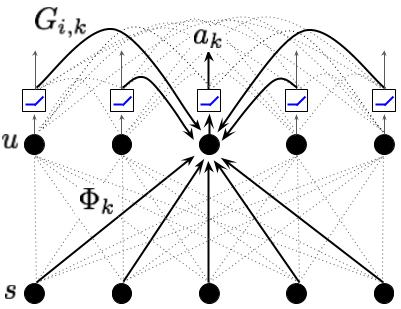
\includegraphics[width=0.4\textwidth]{figures/lca_diagram.png}
    \caption{\textbf{LCA architecture.} The LCA network includes feedforward driving connections, $\Phi$ as well as a lateral connectivity matrix, $G$. The input, $s$, is a vector of pixels, which is the lower row of black dots. The neurons are the upper row of black dots and have internal states, $u$. The dark arrows are connections for neuron $k$. All other connections are denoted by dotted lines.}
    \label{fig:ch2_lca_diagram}
\end{figure}

We wish for our neuron activations to minimize the energy function described in equation \eqref{eq:ch2_sparse_energy}. This will be accomplished via gradient descent. To illustrate the derivative, we first express the energy function in subscript notation:

\begin{equation}\label{eq:ch2_subscript_sparse_energy_func}
    E(t) = \tfrac{1}{2} \sum\limits_{i=1}^{N} \left[ s_{i} - \sum\limits_{j=1}^{M}a_{j}(t) \Phi_{i,j} \right]^{2} + \lambda \sum\limits_{j=1}^{M} C(a_{j}(t))
\end{equation}

and then we take the derivative with respect to an individual neuron's activity, $a_{k}(t)$. Since we ultimately want to do gradient \textit{descent}, we will write the negative derivative:

\begin{align}\label{eq:ch2_lca_deda_extended}
\begin{split}
    - \frac{\partial E(t)}{\partial a_{k}(t)}
    =
        &\sum\limits_{i=1}^{N} S_{i} \Phi_{i,k} -
        \Phi_{i,k}\sum\limits_{j=1}^{M}a_{j}(t) \Phi_{i,j} -
        \lambda \sum\limits_{j=1}^{M}\frac{\partial C(a_{j}(t))}{\partial a_{k}(t)} \\
    =
        &\sum\limits_{i=1}^{N} \left[ s_{i} \Phi_{i,k} -
        \sum\limits_{j \neq k}^{M} \Phi_{i,k} \Phi_{i,j} a_{j}(t) - \Phi_{i,k}\Phi_{i,k}a_{k}(t) \right] -
        \lambda \frac{\partial C(a_{k}(t))}{\partial a_{k}(t)}
\end{split}
\end{align}

We constrain the model to have unit norm dictionary elements in the pixel dimension, $||\phi_{i}||_2^2 = 1$. This means that the $\sum_{i=1}^{N}\Phi_{i,k}\Phi_{i,k}a_{k}(t)$ term in equation \eqref{eq:ch2_lca_deda_extended} reduces to $a_k(t)$:

\begin{equation}\label{eq:ch2_lca_deda}
    -\frac{\partial E(t)}{\partial a_{k}(t)} =
    \sum\limits_{i=1}^{N} \left[ s_{i} \Phi_{i,k} -
    \sum\limits_{j \neq k}^{M} \Phi_{i,k} \Phi_{i,j} a_{j}(t) \right] - a_{k}(t) -
    \lambda \frac{\partial C(a_{k}(t))}{\partial a_{k}(t)}
\end{equation}

$E(t)$ and $a(t)$ both vary in time, but in future sections we will drop the time variable to improve the equation readability. In this scenario, we can imagine a constant input signal, $s$, and a constant set of dictionary elements, $\Phi$. Given these constants, we want the system to evolve over time to produce an optimal set of activations, $a$. Equation \eqref{eq:ch2_subscript_sparse_energy_func} gives us the energy at each time point during this inference process. Each neuron has a corresponding dictionary element, $\phi_{k}$, which is a vector that indicates the connection strength to each pixel in the input. In the literature this is also referred to as the strength of the synaptic connections between the neuron and each input pixel, or the neuron's feed-forward receptive field. In this model, we are going to find a sparse code for each individual image patch. Additionally, all $M$ neurons will be connected to the same image patch, $s$ (i.e. the model is ``fully-connected''). The model neuron has a driving excitatory input, which we will denote $b_{k} = S\phi_{k} = \sum_{i=1}^{N}s_{i} \Phi_{i,k}$. This is the projection of the input image onto the neuron's corresponding dictionary element. The stronger the similarity between the input, $s$, and the dictionary element, $\phi_{k}$, the stronger the driving excitatory input. Each neuron also receives inhibition from every other active neuron. The magnitude of inhibition is partially set by an $M \times M$ Gramian matrix, $G$. The matrix evaluates to the inner product of the each neuron's dictionary element with all other neurons' dictionary elements, $G = \Phi^T\Phi$, such that each element in $G$ gives the overlap in pixel space between two dictionary elements, $G_{i,j} = \sum\limits_{n=1}^{N} \Phi_{n,i}\Phi_{n,j}$. The total inhibition onto a neuron is also scaled by how active the inhibiting neuron is.

Next, we define a new function that maps the activity for a neuron and the sparsity cost function to a scalar. This function can be thought of as the self inhibition that increases as the value of $a_{k}$ increases:

\begin{equation}\label{eq:ch2_hopfield_t_func}
  f_{\lambda}(a_{k}(t)) = a_{k}(t) + \lambda \frac{\partial C(a_{k}(t))}{\partial a_{k}(t)}
\end{equation}

Self inhibition imposes sparsity by penalizing the neurons own output, which is different from the sparsity inducing input from other laterally connected neurons. Now we can write the partial derivative of our energy function (equation \eqref{eq:ch2_subscript_sparse_energy_func}) in terms of our new variables:

\begin{equation}\label{eq:ch2_lca_deda_simple}
    - \frac{\partial E(t)}{\partial a_{k}(t)} =
    b_{k} -
    \sum\limits_{j \neq k}^{M} G_{k,j} a_{j}(t) -
    f_{\lambda}(a_{k}(t)).
\end{equation}

At this point we could update $a(t)$ using gradient descent following equation \eqref{eq:ch2_lca_deda_simple} to produce a sparse code from an input signal. However, a more biologically consistent solution would be to have the model neuron maintain an internal state, analogous to a biological neuron's membrane potential. The model neuron could then only produce output when its membrane potential exceeded some threshold. This has better correspondence to biology and it gives the neurons sub-threshold dynamics that influences their activity (see section \ref{sec:ch2_lca_properties}) when compared to directly using equation \eqref{eq:ch2_lca_deda_simple}. Following this logic, Rozell et al. \citeyearpar{rozell2008sparse} define an internal state variable, $u_{k}(t)$ that represents the membrane potential for neuron $k$ at time $t$. When a neuron's potential climbs above some threshold, it communicates in the form of an activation, $a_{k}(t)$, which is analogous to a spike rate\footnote{Neuroscientists often use the spike rate, or number of spikes per fixed unit of time, as a measure of the overall activity of a neuron. The LCA is not a spiking network, but when comparing to biological neurons (e.g. in the work by \cite{zhu2013visual} and in section \ref{sec:ch4_selectivity_efficiency}) we make a direct analogy between the activity of the LCA neuron and the biological neuron's spike rate. Spiking versions of sparse coding have been explored by \parencite{zylberberg2011sparse, olshausen2003learning}.}. Only these excited neurons can contribute to the image code and reconstruction. Ultimately, the network of neurons should still descend the energy function from equation \eqref{eq:ch2_subscript_sparse_energy_func}, so we define the neuron's state dynamics to be governed by the following equation:

\begin{align}\label{eq:ch2_u_dot}
\begin{split}
    \dot{u_{k}}(t) &\propto - \frac{\partial E(t)} {\partial a_{k}(t)} \\
    \dot{u_{k}}(t) &= \frac{1}{\tau} \left[b_{k} - \sum_{m \neq k}^{M}G_{k,m}a_{m}(t) - f_{\lambda}(a_{k}(t)) \right],
\end{split}
\end{align}

\noindent where $\tau$ is a proportionality constant that represents the time constant of the dynamics.

In order to have a complete description of the model, we need to describe a relationship between $u$ and $a$. Earlier the $f_{\lambda}(a_{k}(t))$ term was described as a self inhibition term that encourages sparsity. Another way to enforce self inhibition is to introduce a membrane leak term. If we assign the internal state, $u_{k}(t)$, to this function:

\begin{equation}\label{eq:ch2_u_func_a}
    u_k(t) = f_{\lambda}(a_{k}(t)),
\end{equation}

\noindent then we can think of our neuron as a leaky integrator. We can also invert the function to get our neuron's output activity:

\begin{displaymath}\label{eq:ch2_a_fu_thresh}
    a_{k}(t) = f_{\lambda}^{-1}(u_{k}(t)) := T_{\lambda}(u_{k}(t)).
\end{displaymath}

This gives us the LCA neuron update equation:
\begin{equation}\label{eq:ch2_u_dot_full}
    \dot{u_{k}}(t) = \frac{1}{\tau} \left[\overbrace{b_{k}}^\text{Driving excitation} - \overbrace{\sum_{m \neq k}^{M}G_{k,m}a_{m}(t)}^\text{Lateral Inhibition} - \overbrace{u_{k}(t)}^\text{Leak} \right],
\end{equation}

\noindent or equivalently

\begin{displaymath}
    \tau \dot{u_{k}}(t) + u_{k}(t) =  b_{k} - \sum_{m \neq k}^{M}G_{k,m}a_{m}(t).
\end{displaymath}

When the neuron's membrane potential passes over a threshold, defined by $T_{\lambda}(u_{k}(t)) = f_{\lambda}^{-1}(u_{k})$, it becomes active:

\begin{equation}\label{eq:ch2_a_thresh}
  a_{k}(t) = T_{\lambda}(u_{k}(t)).
\end{equation}

For this expression to perform gradient descent on the energy function, $a$ must be a monotonically increasing function of $u$. Rozell et al. \citeyearpar{rozell2008sparse} describe the relationship between the sparseness cost penalty, the neuron activity, and the internal membrane potential via a thresholding function. The thresholding function can take various forms that determine the exact nature of the sparseness penalty. For the $l_{1}$ penalty, Rozell et al. \citeyearpar{rozell2008sparse} use a soft thresholding function:

\begin{equation}\label{eq:ch2_lca_threshold_func}
    T_{\lambda}(u_{k}(t)) = \left\{
    \begin{aligned}
        u_{k}(t)+\lambda,\;\; &u_{k}(t)\; <\; -\lambda \\
        0,\;\; &-\lambda < u_{k}(t)\; <\; \lambda \\
        u_{k}(t)-\lambda,\;\; &u_{k}(t)\; >\; \lambda
    \end{aligned}
    \right.
\end{equation}

Here $\lambda$ indicates the sparseness penalty trade-off as well as the threshold that the membrane potential must surpass for the neuron to become active. An illustration of how one gets to the thresholding function from the $l_{1}$ penalty is given in figure \ref{fig:ch2_lca_thresh}. With the internal state dynamics from equation \eqref{eq:ch2_u_dot_full} and the thresholding function in equation \eqref{eq:ch2_lca_threshold_func}, we have defined a network that settles to a sparse code, $a$, which represents the input signal. For all of the work in this thesis, we will diverge from the implementation in \parencite{rozell2008sparse} and implement a rectified version of the thresholding function. That is, from equation \eqref{eq:ch2_lca_threshold_func}, the first term for when $u_{k}(t) < -\lambda$ is set to $T_{\lambda}(u_{k}(t))=0$. This adds a higher degree of nonlinearity, and is important for implementing hierarchical sparse coding models.

\begin{figure}[h]
    \centering %center using container as reference, instead of the whole text
    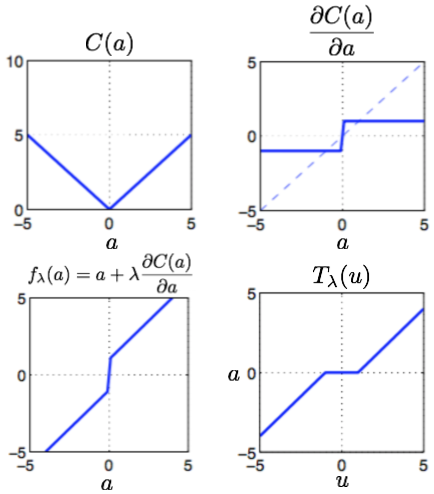
\includegraphics[width=0.4\textwidth]{lca_cost_graphs.png}
    \caption{\textbf{Deriving the LCA thresholding function.} Starting from a pictorial view of the $l_{1}$ cost function, one can derive the self inhibition term from equation \eqref{eq:ch2_u_func_a} and invert it to see the thresholding function described in equation \eqref{eq:ch2_lca_threshold_func}. The value of $\lambda$ dictates the range of allowable sub-threshold membrane potentials, $u_{k}$, before the neuron becomes active.}
    \label{fig:ch2_lca_thresh}
\end{figure}

In addition to finding a sparse code, we are also interested in learning a set of dictionary elements, $\Phi$. This can be done by performing gradient descent on equation \eqref{eq:ch2_sparse_energy} using the coefficient values obtained with the LCA. This yields

\begin{equation}\label{eq:ch2_phi_update}
    \Delta \phi_{k} = \eta (s - \hat{s}) a_{k},
\end{equation}

\noindent where $\eta$ is the learning rate and $\hat{s}$ is the image reconstruction. To recap, for a given image sample we first find our image code, $a$, for a fixed dictionary, $\Phi$, and then using that code to update the dictionary with equation \eqref{eq:ch2_phi_update}.

% TODO diagrams with math comparing feed-forward network to LCA network?
%https://docs.google.com/presentation/d/1Vzk_fVGO-ERQDjKWRvzuHpV6YGwUriD6NyJNpf-WbVE/edit#slide=id.g4f9127c786_0_76

\subsection{The Convolutional LCA}

\begin{figure}[h]
    \centering
    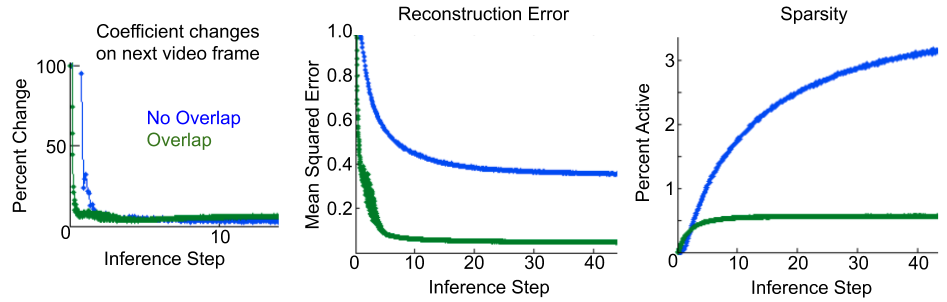
\includegraphics[width=\textwidth]{figures/lca_conv_benefits.png}
    \caption{\textbf{The convolutional LCA has unique coding properties.} The convolutional LCA (overlap, green lines) has better encoding properties than the patch-based LCA (no overlap, blue lines) in terms of stability and energy. We hypothesize that this is an effect of global competition across the image that is afforded by the convolutional architecture. Note that the patch-based LCA is still sharing weights between patches; it is acting as if each patch was encoded independently with the same model. For video input, we recorded the percent change in coefficients from one frame to the next as a function of the number of inference steps performed on each frame. The left plot shows that convolutional variant is more stable earlier in inference, and approximately equally stable after both variants have converged. Additionally, the convolutional LCA settles to a lower mean squared error between the input and reconstruction (middle plot), and is more sparse (right plot) than the patch-based model. This figure was reproduced from unpublished work done with the Kenyon lab \parencite{paiton2013deep}.}
    \label{fig:ch2_lca_conv_benefit}   
\end{figure}

In this thesis, unless otherwise noted, it should be assumed that we are using the fully-connected variant of the LCA, in which each neuron is connected to every pixel in the input. However, the LCA can also be easily extended to be convolutional to scale it up to larger images. There are benefits to using convolutional over fully-connected LCA: it is more amenable popular GPU computing architectures, it converges to lower minima, and it is more stable when encoding video. However, some drawbacks are that it no longer has a straight forward analog hardware implementation and it diverges from the type of connectivity we see in the brain. A possible better alternative to convolution would be to use local (i.e. tiled) connectivity, as was done in \parencite{le2011building} and \parencite{ngiam2010tiled}. At the time of writing we are unaware of any attempt to use this type of connectivity with the LCA.

We will occasionally use the convolutional LCA to scale up experiments to larger inputs. For a neural-network oriented introduction to convolution, see \parencite{goodfellow2016deep}. The convolution will be parameterized by the kernel size, number of kernels, and stride. If the stride is equal to the patch size (i.e. no overlap), then this model implements the regular patch-based LCA that operates on an entire image worth of patches independently, but simultaneously.

For the convolutional LCA, we write our energy function in terms of a ``deconvolution'', or transposed convolution \parencite{zeiler2010deconvolutional}:

\begin{equation}
    E = \frac{1}{2} || s - a \circledast \Phi ||^{2}_{2} + \lambda ||a||_{1},
\end{equation}

\noindent where $\circledast$ is the transposed convolution operator. We also rewrite the membrane update equation to be in terms of a residual error convolved with the weight vector:

\begin{equation}\label{eq:ch2_conv_lca_dynamics}
   \tau \dot{u_{k}} + u_{k} = e \ast \Phi_{k} + a_{k},
\end{equation}

\noindent where $\ast$ is convolution and $e = s - \hat{s}$ is the residual error. In this variant, the driving force to the neurons is the error, instead of the $b_{k}$ term in equation \eqref{eq:ch2_lca_deda_simple}. This means that every neuron that is competing for the image reconstruction will contribute to driving neuron $k$, even if it is in a different convolutional position. The effects of this global competition across the image appear to give the model an advantage in terms of finding an energy minima and stability, which we demonstrate in figure \ref{fig:ch2_lca_conv_benefit}.


\subsubsection{A note on convolutional overcompleteness}
In patch-based sparse coding, we compute the network overcompleteness by dividing the number of neurons by the number of pixels. However, with convolutional sparse coding there is a caveat that the neighboring inputs have shared weights. Therefore, directly expressing the overcompleteness as number of outputs / number of inputs misrepresents the number of unique weights in the model. Even more nuanced is that the LCA typically learns weights that tile all possible positions in the image patch, which is not as necessary with a convolutional model since the convolution operation translates weights across the image. As a result, all weights learned with convolution tend to be centered in their patch. With all of this in mind, we will denote convolutional overcompleteness as the number of kernels divided by the product of the horizontal (x) and vertical (y) strides: $o = \tfrac{f}{s_{x}*s_{y}}$. Therefore, within reasonable parameter ranges, you can effectively increase the overcompleteness by increasing the number of kernels or by decreasing the stride, which is important when considering computational constraints \parencite{schultz2014replicating}. From this we can also conclude that overcompleteness is not dependent on the patch size, which has been exploited for learning disparity selective neurons that require large receptive fields \parencite{lundquist2016sparse}.


\subsection{Postdictions from the LCA}
% TODO: this paragraph references sec:ch2_alternative_image_coding_models after referencing linear/nonlinear neuron models. I don't currently include a discussion on those models in that section.
%TODO: note haider et al work and adesnik work at the end of this paragraph
In their landmark paper, Olshausen and Field \citeyearpar{olshausen1996emergence} show that the sparse coding model learns oriented, band-pass receptive fields.
These are well matched to fits of the linear approximations of receptive fields of mammalian V1 simple cells obtained via spike-triggered averaging \parencite{hateren1998independent}.
They argue that this supports the hypothesis that the V1 neural population encodes visual stimulus using an efficient wavelet-like dictionary.
This result has been replicated a number of times with various types of sparse coding models \parencite{zylberberg2011sparse, zylberberg2013sparse, rehn2007network}.
As a followup to this study, \parencite{zhu2013visual} show that the LCA network also exhibits a variety of extra-classical (i.e. non-linear) receptive field effects, including end-stopping, cross-orientation inhibition, and surround suppression.
This is an important finding, as it shows that a single LCA network trained on natural scenes matches many linear and non-linear empirical effects found with biological neurons.
Most studies of these non-linear effects employ unique models that are extended from the classic linear/non-linear neuron model for each effect found, while Zhu and Rozell are able to demonstrate many effects with a single model.
In chapter 4 we will argue that these effects result from the explaining away process during sparse inference. %TODO: fix chapter refs
In \parencite{vinje2000sparse}, the authors find that stimulating the nCRF (non-classical receptive field) with naturalistic stimuli causes pairs of V1 neurons to become more decorrelated in their response.
They observed ``dramatically increased sparseness'' when stimulating nCRFs, and suggest that a consequence of this ``is increased independence of the responses across cells''.

As we will expand on in chapter 4, the LCA makes explicit predictions about the existence (and necessity) of population non-linearities among V1 neurons, which facilitate unique responses to natural image stimuli. %TODO: Fix chapter refs
The model gives important attribution for inhibitory lateral connectivity in V1 \parencite{zhu2015modeling}.
In addition to the obvious energy saving motivation for sparse activity, it has been argued that limiting the number of active neurons can result in a more explicit code that is easier to read out by downstream neurons \parencite{olshausen2003principles}.
We will explore this in more detail in later chapters.


\section{Properties of the LCA trained on natural images}\label{sec:ch2_lca_properties}
\subsection{Features learned}
% TODO: Retrain using a different data sample to see if spatial freqs stay anisotropic
% TODO: Are verticle / horizontal RFs also more frequent in v1?
It has been shown previously that sparse coding will learn a dictionary of features that tile spatial position, frequency, and orientation \parencite{olshausen1996emergence, olshausen1997sparse}. We reproduce this finding while also varying the overcompleteness of the model in figure \ref{fig:ch2_lca_overcompleteness_tiling}. We find that as overcompleteness increases, the density of the tiling also increases. Additionally, the model learns higher spatial frequency features and a more even distribution of orientations when more overcomplete. It is also interesting that the models tend to learn significantly more features that are aligned with the vertical and horizontal axis of the input images, which is well matched to image statistics \parencite{switkes1978spatial, torralba2003statistics}. The spatial frequencies also have anisotropy across the vertical axis, which is maintained as you increase overcompleteness. We suspect this is an artifact of the dataset tested, as all three models were trained from the same image patch samples, although we did not test this hypothesis. We also show in figure \ref{fig:ch2_lca_angle_histograms} that when we increase overcompleteness, the neurons have more similar receptive fields as indicated by a smaller angle between weight vectors.

\begin{figure}[ht]
    \centering
    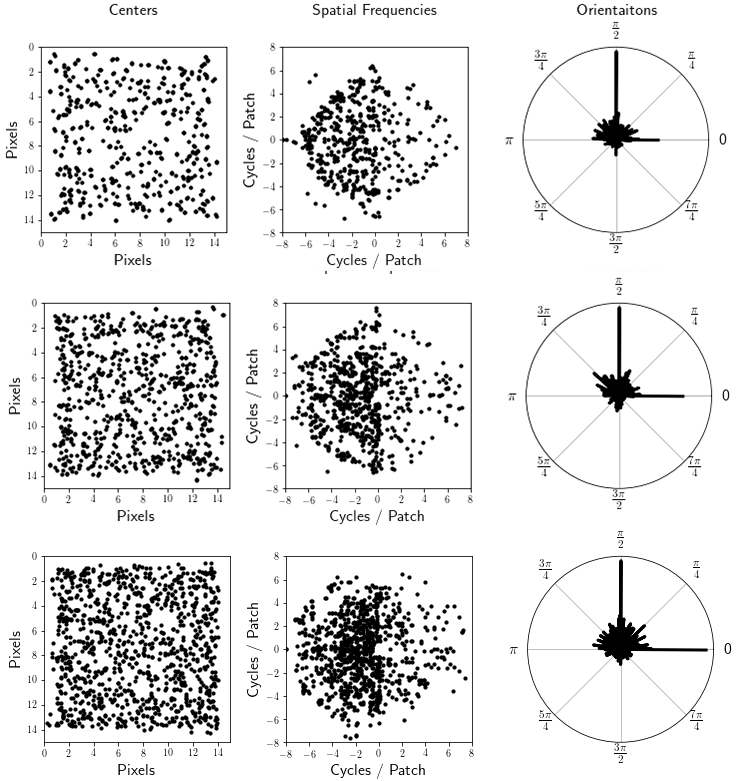
\includegraphics[width=0.8\textwidth]{figures/lca_fits_loc_freq_orien.png}
    \caption{\textbf{Properties of features learned with LCA.} The LCA learns a diverse set of features that tile important signal characteristics when trained on patches from natural scenes. From top to bottom, the rows represent the LCA with 2, 3, and 4 times more neurons than pixels, respectively. From left to right, the columns are the spatial positions, spatial frequencies, and orientations of each function.}
    \label{fig:ch2_lca_overcompleteness_tiling}
\end{figure}

\begin{figure}[h]
    \centering
    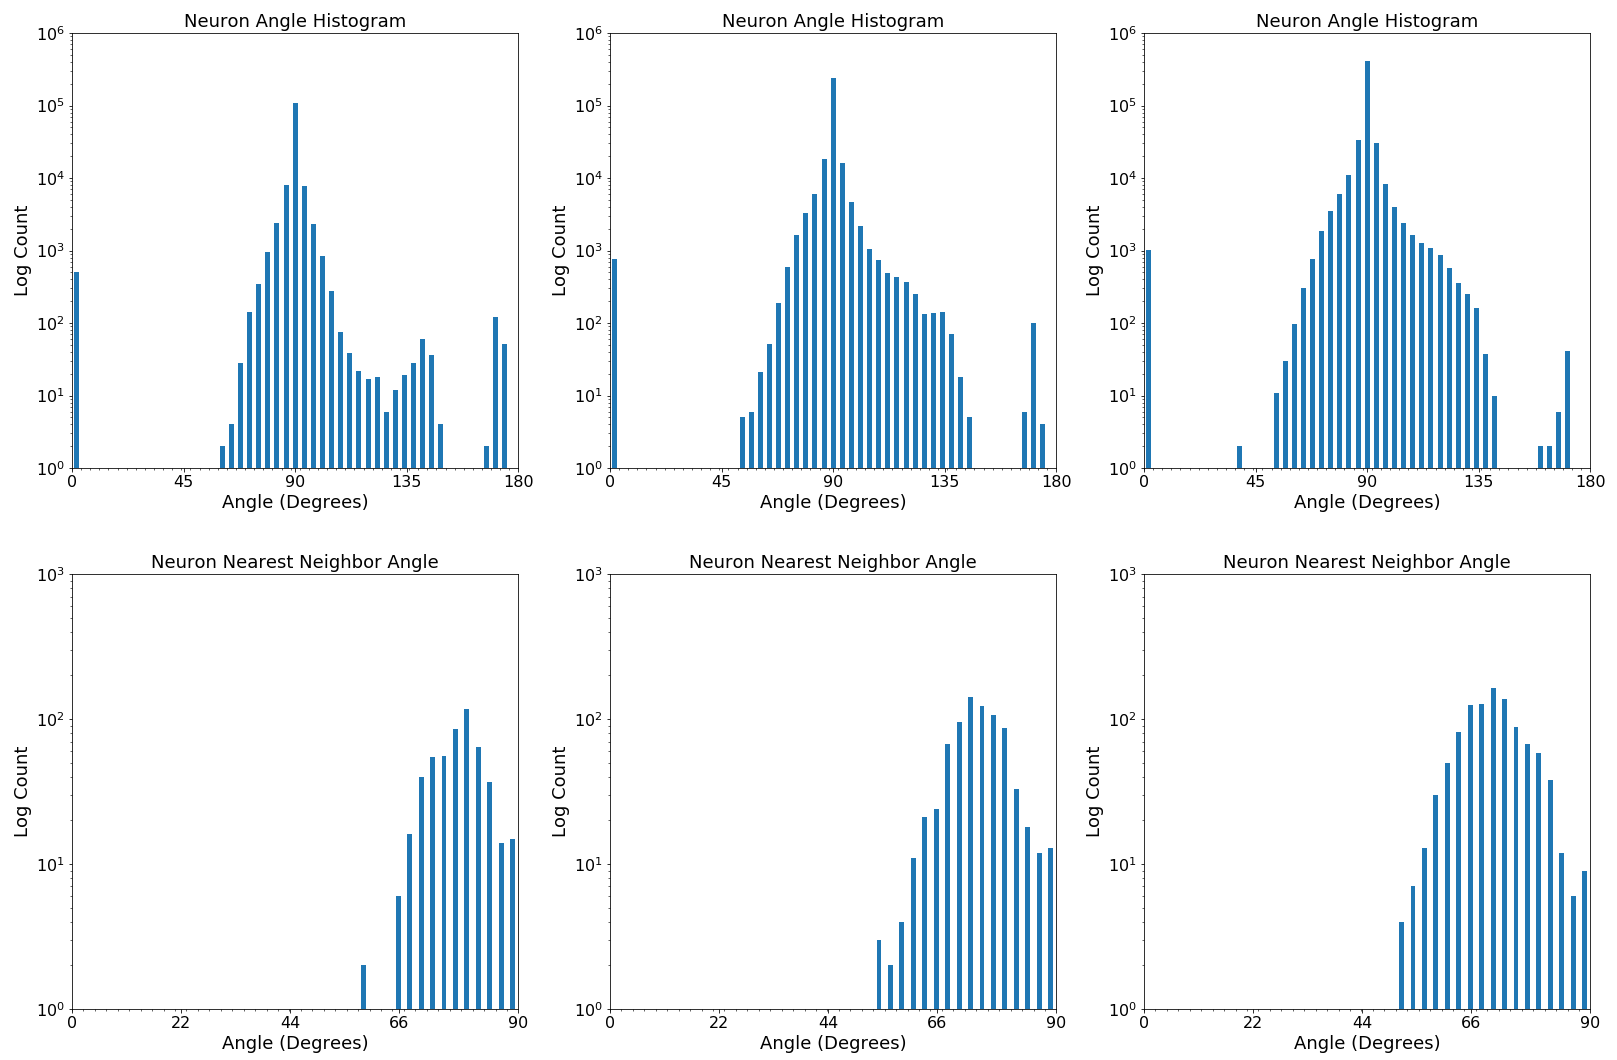
\includegraphics[width=0.9\textwidth]{figures/lca_angle_hists.png}
    \caption{\textbf{The LCA neuron weights are closer as overcompleteness increases.} The top row are histograms of the angles between all pairs of basis functions. The bottom row are histograms of the angles to the nearest neighbor for each neuron. From left to right, we increase the network's overcompleteness such that there are 2, 3, and 4 times more neurons than pixels, respectively. The histograms shift left as we increase overcompleteness, indicating that the weight vectors are closer in angle. This will increase competition among neurons because the Gramian matrix term in equation \eqref{eq:ch2_u_dot_full} will have higher values.}
    \label{fig:ch2_lca_angle_histograms}
\end{figure}


\subsection{Inferring sparse codes of natural images with the LCA}
Inference is a critical component of the sparse coding model.
It gives the model the ability to ``explain away'' causes of the input signals \parencite{olshausen1997sparse} and gives neurons a higher degree of selectivity (see chapter 4). %TODO: Fix chapter refs
Figure \ref{fig:ch2_lca_inference_loss} shows the values of the loss function in equation \eqref{eq:ch2_sparse_energy} through inference, demonstrating that the total loss is reduced.
Notice that the sparse loss starts at zero, indicating that none of the neurons are contributing to the reconstruction.
At the beginning of inference, all of the neurons with weights that have a non-zero inner product with the input will increase their membrane potential without producing any output and without receiving any inhibition from other neurons.
It is only after a neuron passes threshold that it starts producing outputs and inhibiting its neighbors.
These sub-threshold dynamics can result in a better solution than the standard ISTA framework, which turns on all units that have a non-zero inner product with the input at the first inference step \parencite{rozell2008sparse}.

\begin{figure}[h]
    \centering
    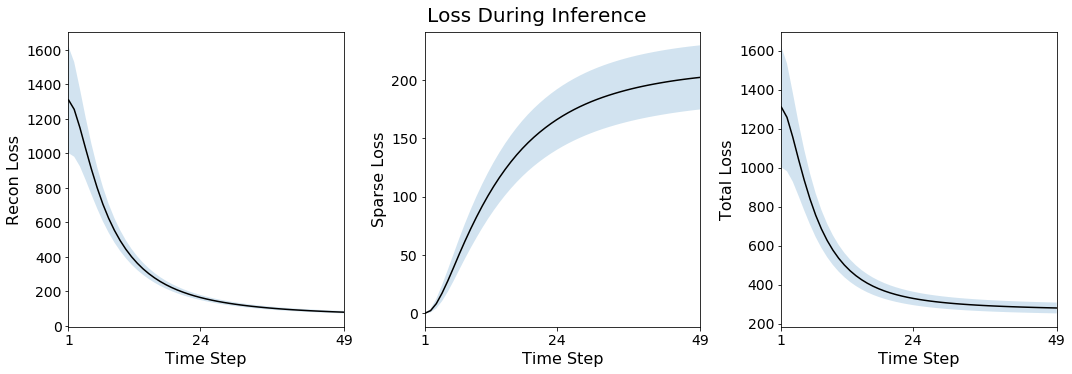
\includegraphics[width=\textwidth]{figures/lca_inference_loss.png}
    \caption{\textbf{LCA inference minimizes the sparse coding energy function.} The black lines represent the mean loss when encoding 50 natural scenes and the blue background represents the standard error of the mean.}
    \label{fig:ch2_lca_inference_loss}
\end{figure}

Figure \ref{fig:ch2_lca_inference_traces} gives us an idea of the inference dynamics for a subset of neurons in the LCA network. Each line in the trace plots represents a different term from equation \eqref{eq:ch2_lca_deda_simple}. Nearly all of the traces follow nonlinear trajectories and have interesting sub-threshold dynamics. Figure \ref{fig:ch2_lca_inference_weights} shows the corresponding weights for each of the neuron traces in figure \ref{fig:ch2_lca_inference_traces}.


\subsection{The hard thresholded LCA has many energy minima}\label{sec:ch2_hard_lca}
It is possible to define a variety of valid threshold functions for converging LCA dynamics. The two primary functions considered in \parencite{rozell2008sparse} are termed ``soft'' and ``hard'' thresholds, which approximate solutions to the $l_{1}$ and $l_{0}$ cost functions, respectively. Much of the work herein is focused on the soft threshold function (equation  \ref{eq:ch2_lca_threshold_func}), primarily for model simplicity. However, the hard thresholded variant is intriguing as it results in a higher degree of non-linearity and solves a harder (non-convex) optimization problem with many equally valid local minima. The rectified hard thresholded LCA model behaves exactly as is described in section \ref{sec:ch2_lca}, except that the thresholding function has been changed to:

\begin{equation}\label{eq:ch2_lca_hard_threshold_func}
    T_{\lambda}(u_{k}(t)) = \left\{
    \begin{aligned}
        0,\;\; &u_{k}(t)\; \leq\; \lambda \\
        u_{k}(t),\;\; &u_{k}(t)\; >\; \lambda
    \end{aligned}
    \right.
\end{equation}

As is described in \parencite{rozell2008sparse}, this variant approximates the $l_0$ cost function for $C(\cdot)$ in equation \eqref{eq:ch2_sparse_energy}. The hard thresholded LCA performs similarly to the soft thresholded variant, except that there is no longer a convex energy landscape with a single global minimum. After some number of inference steps, the LCA settles to a stable minima, but in \parencite{shainin2016sampling} we show that the minima reached by a convolutional, rectified, hard thresholded LCA is not a global minima. It is not clear how the amount of information differs between these minima. However, it has been proposed that the brain could represent likely events in a probabilistic framework \parencite{lee2003hierarchical} and that sampling could be a mechanism for decoding signals in higher cortical areas \parencite{hoyer2003interpreting}.

% TODO: verify the distance metric we used - neurons that turned on / off or neurons that changed activity?
To better understand the energy landscape, we sampled a number of approximately equivalent minima (in terms of energy) for sparse codes produced from weights trained on the CIFAR10 dataset \parencite{krizhevsky2009learning}. We performed this sampling by first allowing the network to settle to a minima for a given image, then perturbing the neuron activations with Gaussian noise, then allowing it to settle again, and repeating for some fixed number of perturbations. We measured the distances between fixed points by counting the number of neurons that changed from active to inactive, which is equivalent to the Hamming distance between binarized (changed threshold or did not) vectors. Figure \ref{fig:ch2_lca_fixed_point_distances} shows that the Hamming distance from the original fixed point to the perturbed fixed point grows as we continue to perturb the network until it reaches a plateau. The figure also shows that the network \textit{always} settles on a different minima.

%TODO: add label to right plot (sample number) and to colorbar (hamming distance)?
\begin{figure}[h]
    \centering
    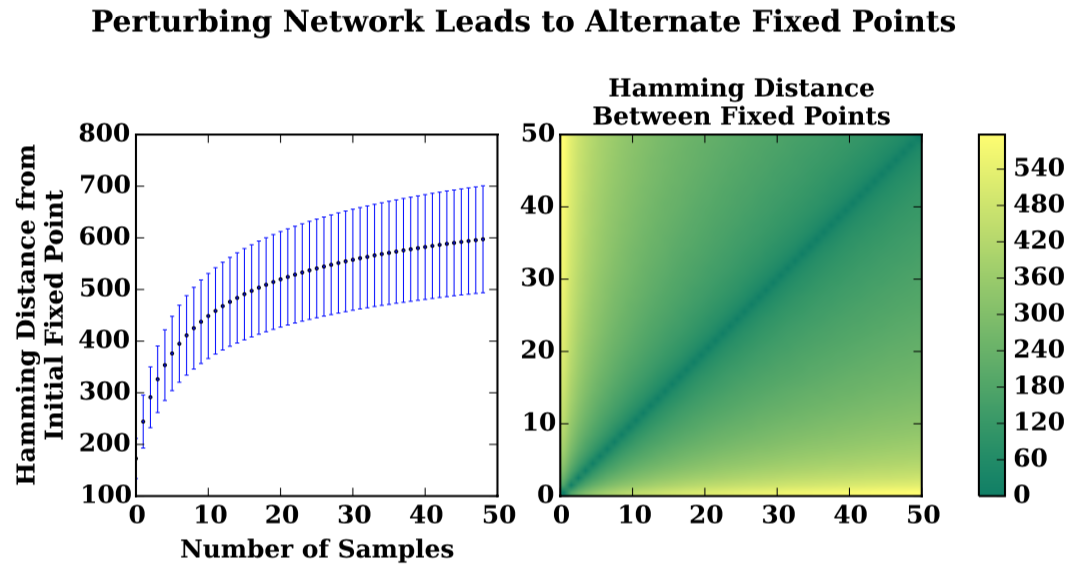
\includegraphics[width=0.75\textwidth]{figures/lca_fixed_point_distances.png}
    \caption{\textbf{Fixed points of the hard thresholded LCA.} The hard thresholded LCA has a number of valid fixed points in terms of the energy defined in equation \eqref{eq:ch2_sparse_energy}. If you allow the model to settle to a minima, and then perturb the latent code with Gaussian noise, it settles to a different minima. On the left we plot the Hamming distance between codes from the original fixed point to the perturbed fixed point after many perturbations. The Hamming distance is measured by assessing how many neurons crossed threshold from active to inactive or vice versa. On the right we plot the Hamming distances between all pairs of fixed points for all perturbations. All of the off-diagonal values are above 0, which indicates that the model always settled to a unique minima after perturbation. This figure was reproduced from unpublished work with permission from \parencite{shainin2016sampling}.}
    \label{fig:ch2_lca_fixed_point_distances}
\end{figure}

In figure \ref{fig:ch2_lca_norms_and_acc}, we show that the $l_{0}$ sparsity of the activations improves as we continue to perturb the input while the reconstruction error remains the same, suggesting that it is finding better minima. To understand the information content of these minima, we trained two layer classifiers on the sparse codes produced after convergence. The first experiment was to average the fixed point vectors together. We show that the classification accuracy increases as we add more fixed points to the average, which implies that there is different information content per fixed point. The second experiment was to search the independent fixed points for whichever produced the highest confidence (in terms of minimum entropy of the classifier's output distribution) and use this single fixed point as input to the network. The right panel in figure \ref{fig:ch2_lca_norms_and_acc} shows that the classifier accuracy improves as we increase the number of candidates in the search. Additionally, we found that the number of perturbations to achieve a fixed point with highest confidence was highly variable (not shown).

\begin{figure}[h]
    \centering
    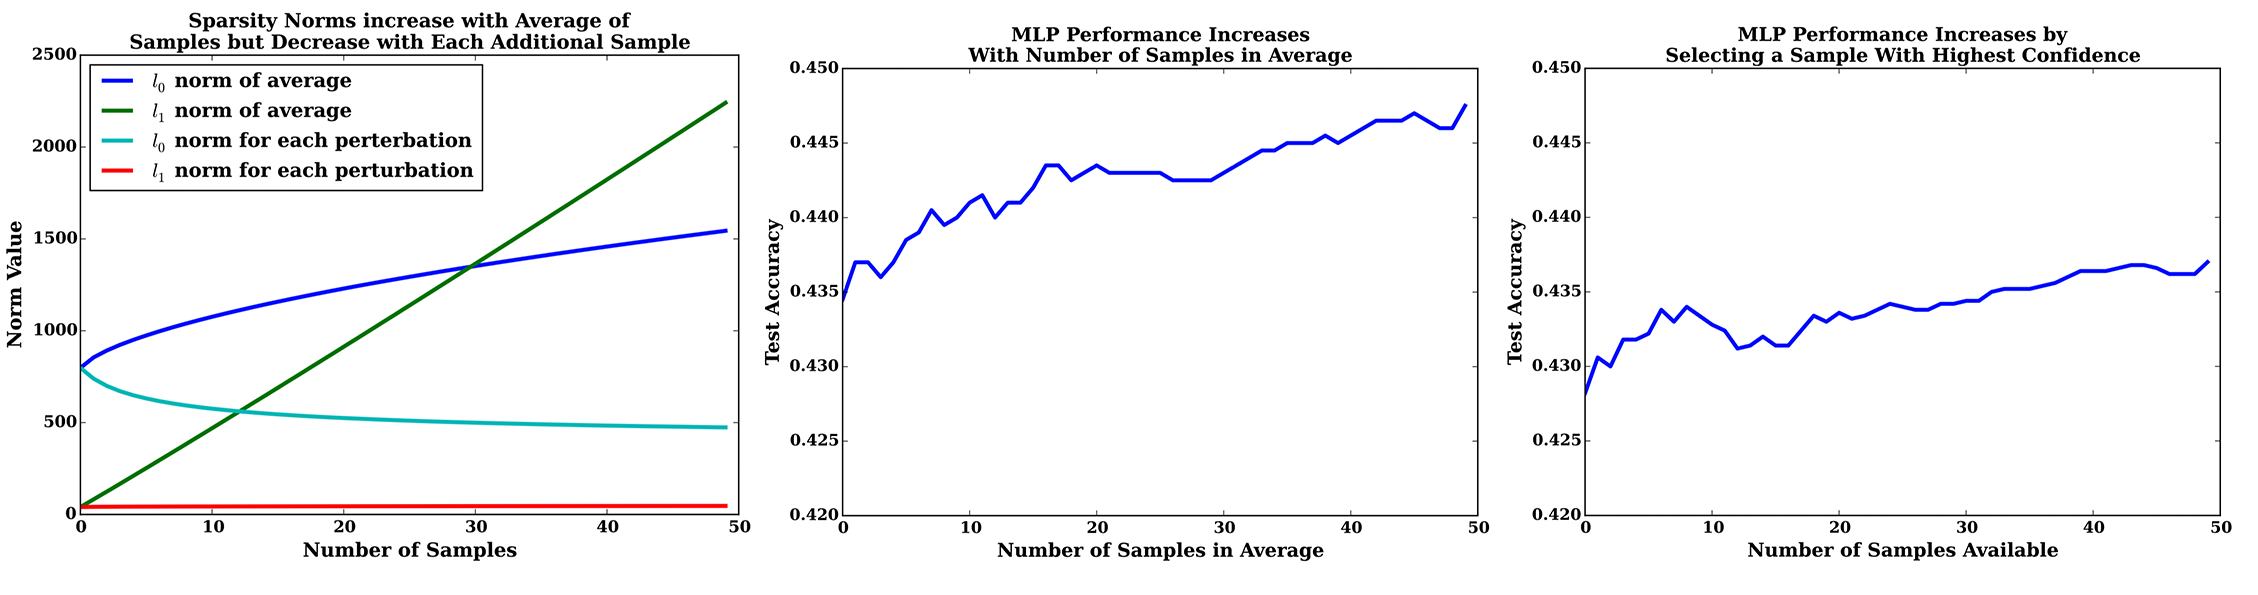
\includegraphics[width=\textwidth]{figures/lca_norms_acc.png}
    \caption{\textbf{Fixed points have different sparsity and contribute unique information for a classification task.} The plot on the left indicates that new fixed points after perturbing the hard thresholded LCA network tend to have fewer active elements. The blue and green lines show that norms increase when we average together the codes from each perturbation, which is to be expected. The cyan and red curves show that as we continue to perturb the activations, the network settles on a minima with approximately equal $l_{1}$ norm and an improved $l_{0}$ ``norm'', or active neuron count. For the middle plot we constructed an averaged vector from each fixed point and used that as the input to a classifier network. The classifier accuracy improves as the number of vectors in the average grows, indicating that there is additional information in the alternate fixed points. As a followup experiment, instead of averaging the fixed points, we searched them to determine which one produces a minimum entropy output from the classifier. This fixed point was then used to determine the class label. The right most figure shows that as you increase the number of samples in the search, the classifier accuracy improves. This figure was reproduced from unpublished work with permission from \parencite{shainin2016sampling}.}
    \label{fig:ch2_lca_norms_and_acc}
\end{figure}


\section{Alternative image coding models}\label{sec:ch2_alternative_image_coding_models}

% TODO:
%\subsection{The linear / non-linear neuron model}
%Simoncelli, etc. Adding components.
% mathematical comparison from L/NL model to RAE & SAE
%
%\subsection{Autoencoders}
%Autoencoders as a NN implementation of L/NL neurons.


\subsection{Predictive coding}
Here we will draw comparisons between the LCA and the predictive coding model \parencite{rao1999predictive}. The LCA encoder is a single layer predictive coding encoder with a linear synthesis function. This is made intuitive by comparing the LCA against the predictive coding model.

The objective of this investigation is to explore the encoding processes for sparse coding and predictive coding assuming that we are given a trained dictionary. In our sparse coding energy function (equation \eqref{eq:ch2_sparse_energy}), we use $\lambda$ as a trade-off penalty between the reconstruction quality and the sparsity constraint. In practice we tune it to maximize network sparsity for a minimum accepted reconstruction quality. In Olshausen and Field \citeyearpar{olshausen1997sparse}, their choice of cost function, $C(.)$, specified a Cauchy distribution for the prior on $a$:

\begin{equation}\label{eq:ch2_cauchy_cost}
  C(a_{i}) = \log(1+a_{i}^{2})
\end{equation}

For a learned dictionary, to encode an input image we compute a coefficient vector, $a$. Our coefficients (neuron activations) adapt to minimize the energy function described in equation \eqref{eq:ch2_sparse_energy}. The standard way to do this is to perform direct gradient descent on the energy function, following equation \eqref{eq:ch2_lca_deda_extended}, which we will rewrite here with a small algebraic change:

\begin{equation}\label{eq:ch2_sc_deda_rewrite}
    - \frac{\partial E(t)}{\partial a_{k}(t)}
    =
        \sum\limits_{i}^{N} \Phi_{i,k} \left(S_{i} - \sum\limits_{j}^{M}a_{j}(t) \Phi_{i,j}\right) -
        \lambda \sum\limits_{j}^{M}\frac{\partial C(a_{j}(t))}{\partial a_{k}(t)}
\end{equation}

A block diagram illustration of this encoding process is given in figure \ref{fig:ch2_lca_pc_comp}.

Much like the sparse coding model, the predictive coding model is a neural network that aims to implement efficient coding for natural visual stimuli \parencite{rao1997dynamic, rao1999predictive}. Although the predictive coding model is described in a more general fashion, the actual implementation used for experiments ends up being strikingly similar to the sparse coding model. Assuming a learned dictionary, the energy equation for the predictive coding model is as follows:

\begin{equation}\label{eq:ch2_pc_energy_func}
        E =
        \tfrac{1}{\sigma_{S}^{2}} \|S - \hat{S} \|_{2}^{2} +
        \tfrac{1}{\sigma_{td}^{2}} \|a - a^{td}\|_{2}^{2} +
        \lambda \sum\limits_{i}^{M}C(a_{i}),
\end{equation}

where $a^{td} = f\left(\Phi^{1T}a^{1}\right)$ represents the top-down feedback and $\sigma_{td}^2$ is the expected Gaussian variance of the $a^{0}$ estimate. As they describe it, this is a combination of the ``sum of squared prediction errors for level 1 and level 2, each term being weighted by the respective inverse variances.'' The energy function also includes a cost on the activations, which for this example will still be derived from the Cauchy prior. A key difference here between this model and the sparse coding model is how the image approximation, $\hat{S}$ is computed. Rao and Ballard describe a non-linear synthesis function, $f(.)$, which is used in the reconstruction:

\begin{equation}\label{eq:ch2_pc_synthesis}
 \hat{S} = \sum\limits_{i}^{M}f(\phi_{i}a_{i})
\end{equation}

If $f(.)$ is the identity function (i.e. $f(a)=a$), then we get the sparse coding reconstruction energy term. Rao and Ballard describe this as a ``lateral inhibition'' model, although the form of synthesis does not actually differentiate between a feedback or lateral inhibition model. In their study, they experiment with both an identity synthesis function, $f(a)=a$, and a hyperbolic tangent synthesis function, $f(a)=tanh(a)$.

Again we can take the derivative of equation \eqref{eq:ch2_pc_energy_func} to get our update rule. In \parencite{rao1999predictive} they include a time constant for the iterative update procedure, which we will leave out for clarity.

\begin{equation}\label{eq:ch2_pc_deda}
    - \frac{1}{2}\frac{\partial E}{\partial a_{k}}
    =
        \frac{1}{\sigma_{S}^{2}}\sum\limits_{i}^{N} \Phi_{i,k} \left(S_{i} - \sum\limits_{j}^{M}a_{j} \Phi_{i,j}\right) -
        \frac{1}{\sigma_{td}^{2}}\sum\limits_{i}^{M}(a_{i}-a_{i}^{td}) -
        \lambda \sum\limits_{j}^{M}\frac{\partial C(a_{j})}{\partial a_{k}}
\end{equation}

Comparing equations \eqref{eq:ch2_pc_deda} and \eqref{eq:ch2_sc_deda_rewrite}, one can conclude that the two differences between the predictive coding model and sparse coding model are the (potential) use of a non-linear synthesis function and a second layer of processing. This is illustrated pictorially in figure \ref{fig:ch2_lca_pc_comp}.

\begin{figure}[H]
    \centering
    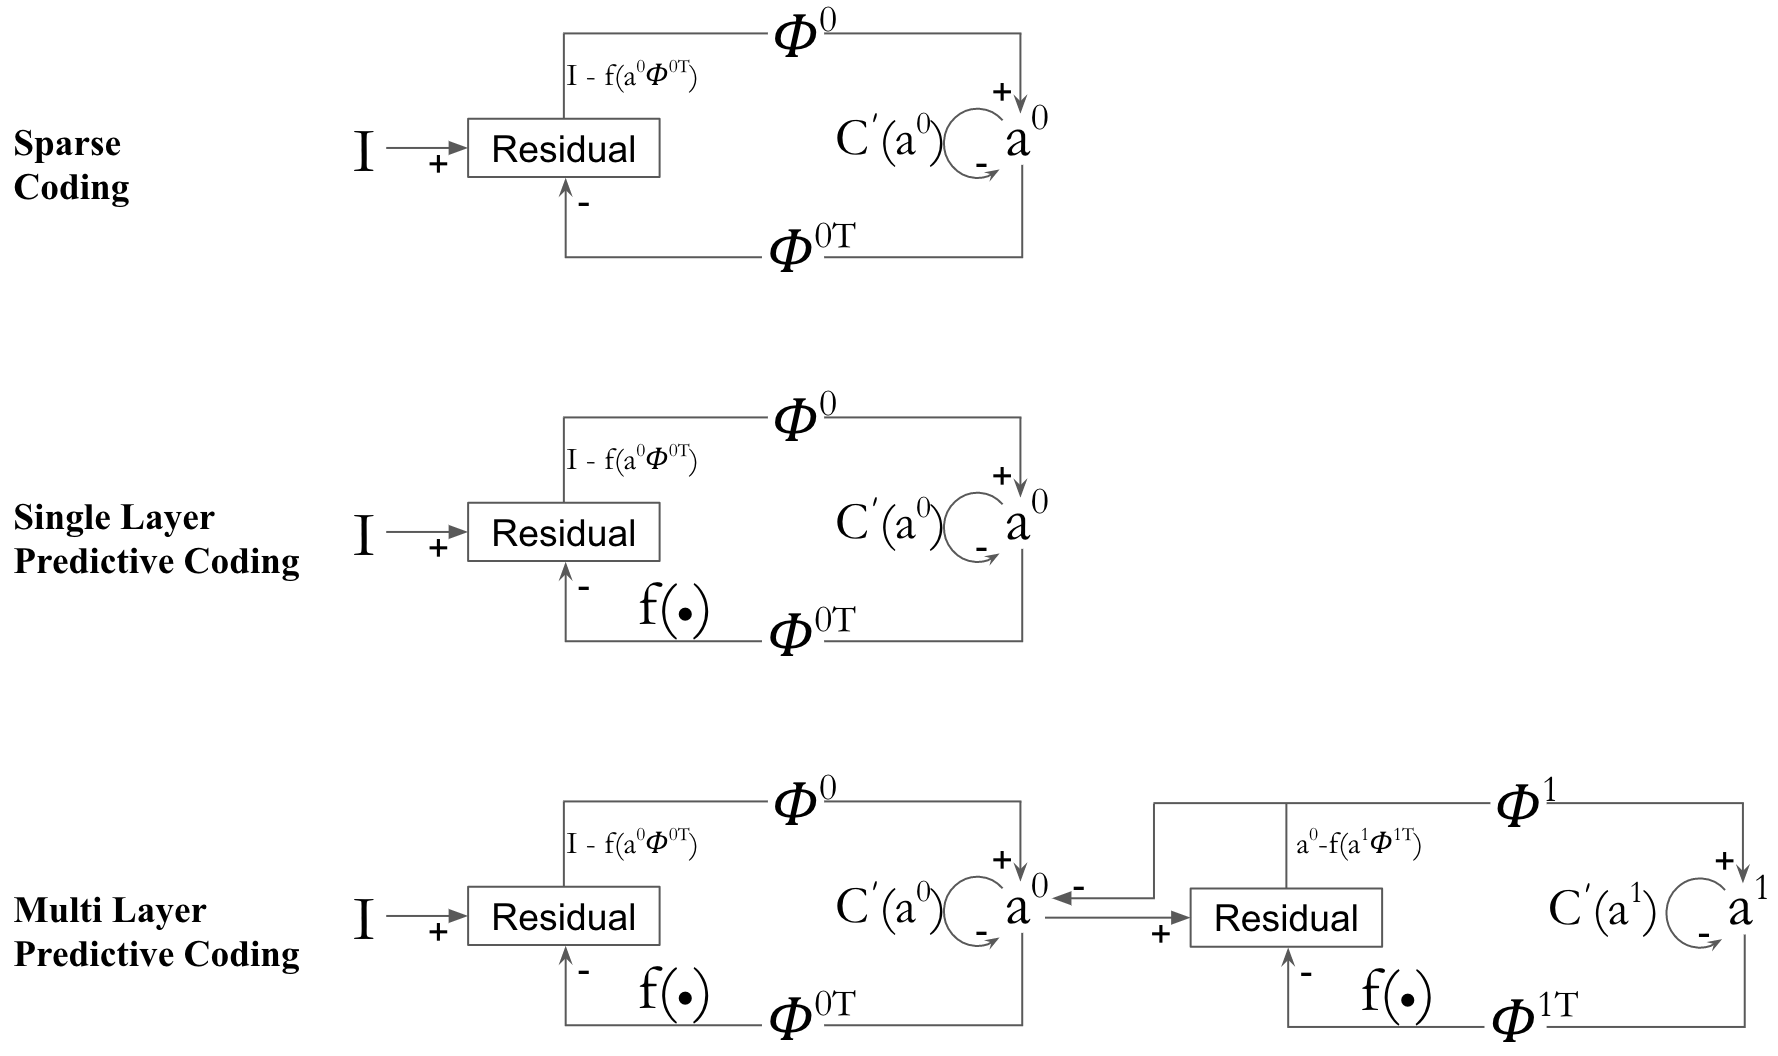
\includegraphics[width=0.9\textwidth]{./figures/lca_pc_model_comparisons.png}
    \caption{\textbf{Comparing the LCA to Predictive Coding.} Sparse approximation can be performed via direct gradient descent on the energy function defined in equation \eqref{eq:ch2_sparse_energy}, which we depict as a dynamic process. Adding a non-linearity to the LCA synthesis function results in a network that is equivalent to a single layer of the predictive coding model. The full model combines two such layers \parencite{rao1999predictive}}
    \label{fig:ch2_lca_pc_comp}
\end{figure}


% TODO:
%\subsection{Iterative Subtraction as a Form of Divisive Normalization} \label{divnorm}
%In their nature publication \cite{rao1999predictive}, Rao \& Ballard suggest that repetitive subtraction of neighboring neuronal activities may produce a net effect similar to divisive normalization. Eero's group has look extensively into divisive normalization - this section is intended to attempt to draw a link between the two.


\subsection{ICA}
Sparse coding and ICA are related algorithms that employ similar linear generative models, but differ critically in their encoding processes. The image code produced by ICA is computed linearly, whereas sparse coding computes the code with a nonlinear inference process. In section \ref{sec:ch4_selectivity_efficiency}, we show that this nonlinear encoding process confers a considerable advantage in coding efficiency and orientation selectivity.

ICA assumes the generative model

\begin{equation}\label{eq:ch2_ica_generative_model}
    s = \Phi a,
\end{equation}

\noindent where $\mathbf{s}$ is an image, $\mathbf{\Phi}$ is a matrix of filters, and $\mathbf{a}$ is a vector of activations that represents the neural code \parencite{bell1997independent}. The goal of ICA is to learn a set of statistically independent filters such that the input data can be reconstructed with minimal error. In ICA, the filter matrix is square and full rank and thus invertible. This allows the ICA activations for a given input to be computed directly as:

\begin{equation}
    \hat{a} = \Phi^{-1}s
\end{equation}

During inference, activations are computed with a single, linear, feed-forward operation. The filter matrix is learned via a non-linear, iterative optimization process to accurately reconstruct the input while maximizing the statistical independence of the filters as measured by the joint entropy of the activations. This process results in filters that are optimized for the higher-order statistical structure in natural scenes.

Sparse coding, however, has a highly non-linear encoding process. The overall optimization procedure involves a fast inner loop in which the coefficients are computed for each data vector and a slower outer loop in which the basis functions are adapted to the statistics of the entire dataset. In the inner loop, coefficients are computed considering the prior on their expected distribution. In ICA, however, the prior plays no role in determining the coefficients, but it does still play an important role in the learning the basis functions.

The ICA learning algorithm is simpler and faster than the sparse coding algorithm because the encoding can be computed from the data in a single feedforward pass. The independent component analysis algorithm of Bell and Sejnowski \citeyearpar{bell1997independent} is formally equivalent to maximum likelihood estimation in the case of no noise and a square system (the dimensionality of the output is equal to the dimensionality of the input). It is easy to generalize this to the case when the number of outputs is less than the number of inputs, but harder the other way around. When the number of outputs is greater than the effective dimensionality of the input the extra dimensions of the output will simply drop out \parencite{livezey2016degeneracy, le2011ica}. While this is not as important for blind separation problems where the number of independent sources is less than or equal to the number of mixed signals, it will become a concern in the representation of images, where overcompleteness is a desirable property \parencite{simoncelli1991shiftable}. The main difference between the Olshausen and Field \citeyearpar{olshausen1996emergence} sparse coding model and the ICA algorithm of Bell and Sejnowski \citeyearpar{bell1997independent} is in the simplifying assumptions they make in order to deal with the intractable integration problem posed by finding the set of basis functions that maximize the likelihood of the inputs given the model defined by those basis functions. Olshausen and Field’s algorithm assumes low-noise and a peaky, unimodal distribution on the joint probability between the image and the sparse code given the model in order to justify evaluating it at the maximum. Bell and Sejnowski limit the dimensionality of the code to equal the dimensionality of the input, assume no noise, and enforce an orthogonal set of basis functions so that the integral becomes tractable and can be analytically computed.

% TODO: BF learned with ICA vs complete LCA ; the LCA is still non-linear encoding when complete.

\section{Conclusion}
In this chapter we derived the LCA from a probabilistic perspective. We then showed the features learned by the LCA when trained on natural scenes and highlighted some interesting properties of the inference process. Finally, we compared the LCA to alternative image coding models. In the next chapter we will extend the LCA model to a semi-supervised learning framework and a hierarchical framework. In the following chapter we demonstrate how a geometric analysis technique can be used to explain the LCA's high degree of robustness to noise and selectivity when compared to alternative models.

\begin{figure}[ht]
    \centering
    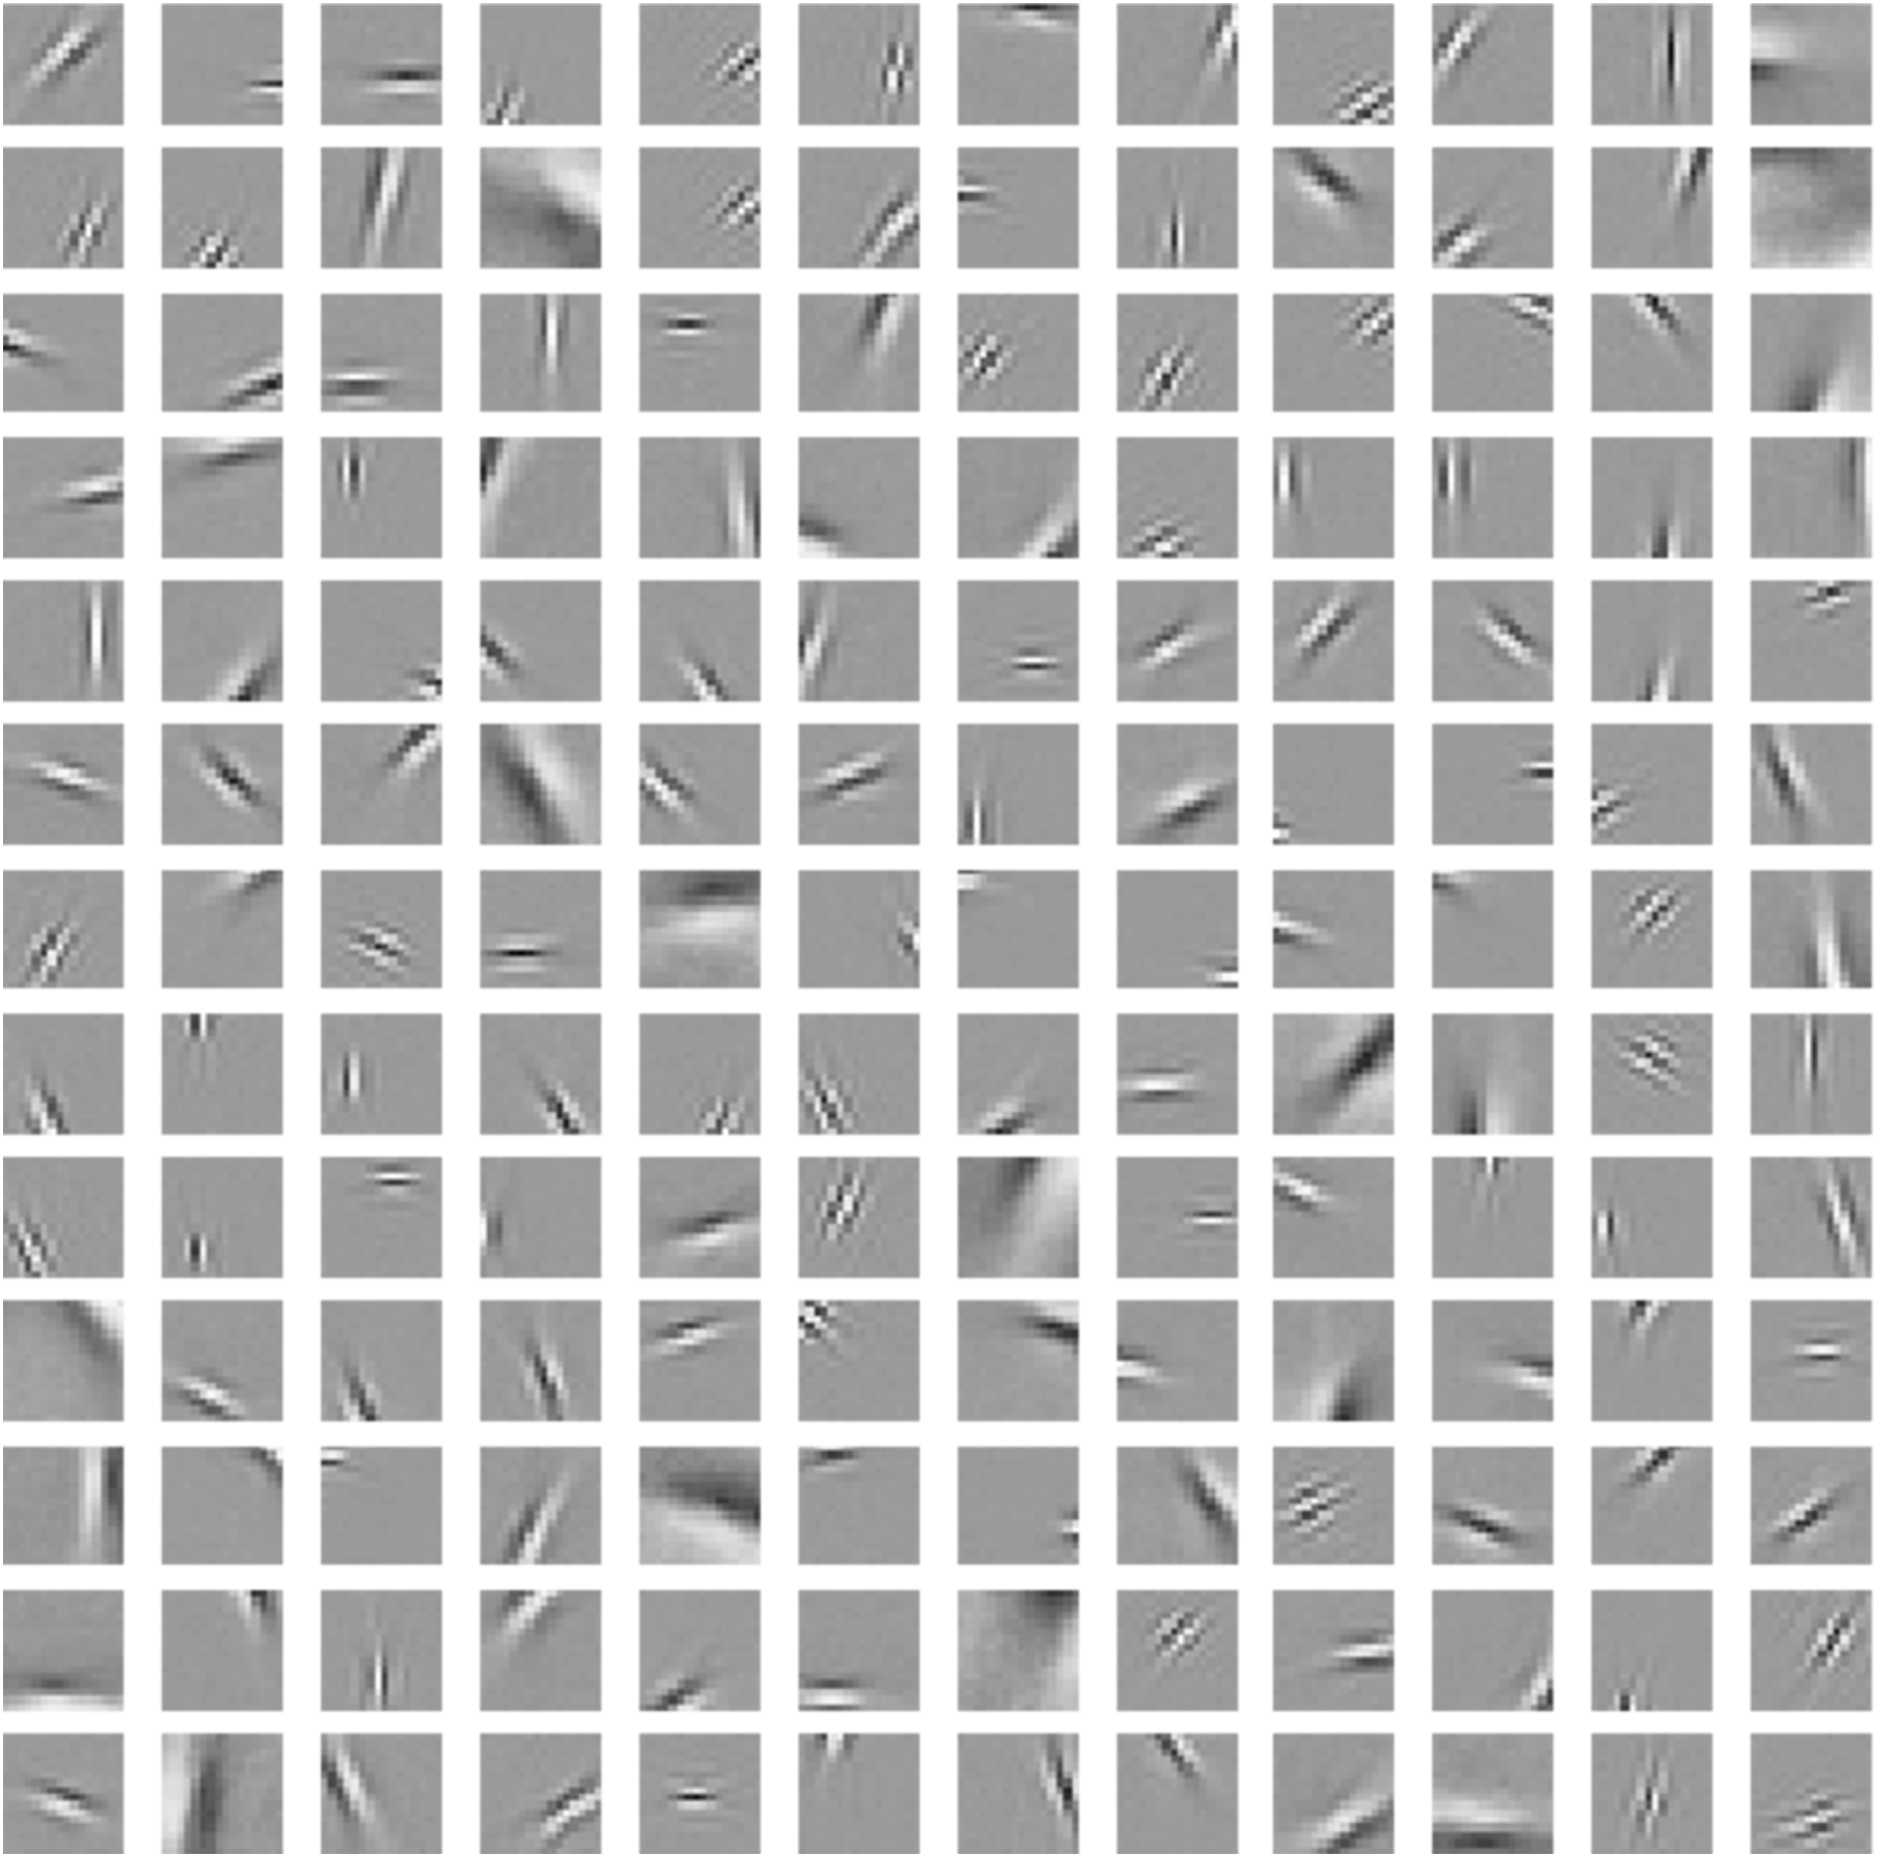
\includegraphics[width=0.5\textwidth]{figures/lca_inference_weights.png}
    \caption{\textbf{Weights learned when the LCA is trained on natural scenes.} Like other sparse coding variants, dictionary learning with LCA inference produces weights that have a high degree of correspondence to those recorded from mammalian V1 \parencite{zylberberg2011sparse, rehn2007network, olshausen1997sparse}. The weights in this plot correspond to the same neurons as were used to generate the traces in figure \ref{fig:ch2_lca_inference_traces}.}
    \label{fig:ch2_lca_inference_weights}
\end{figure}

\begin{figure}[h]
    \centering
    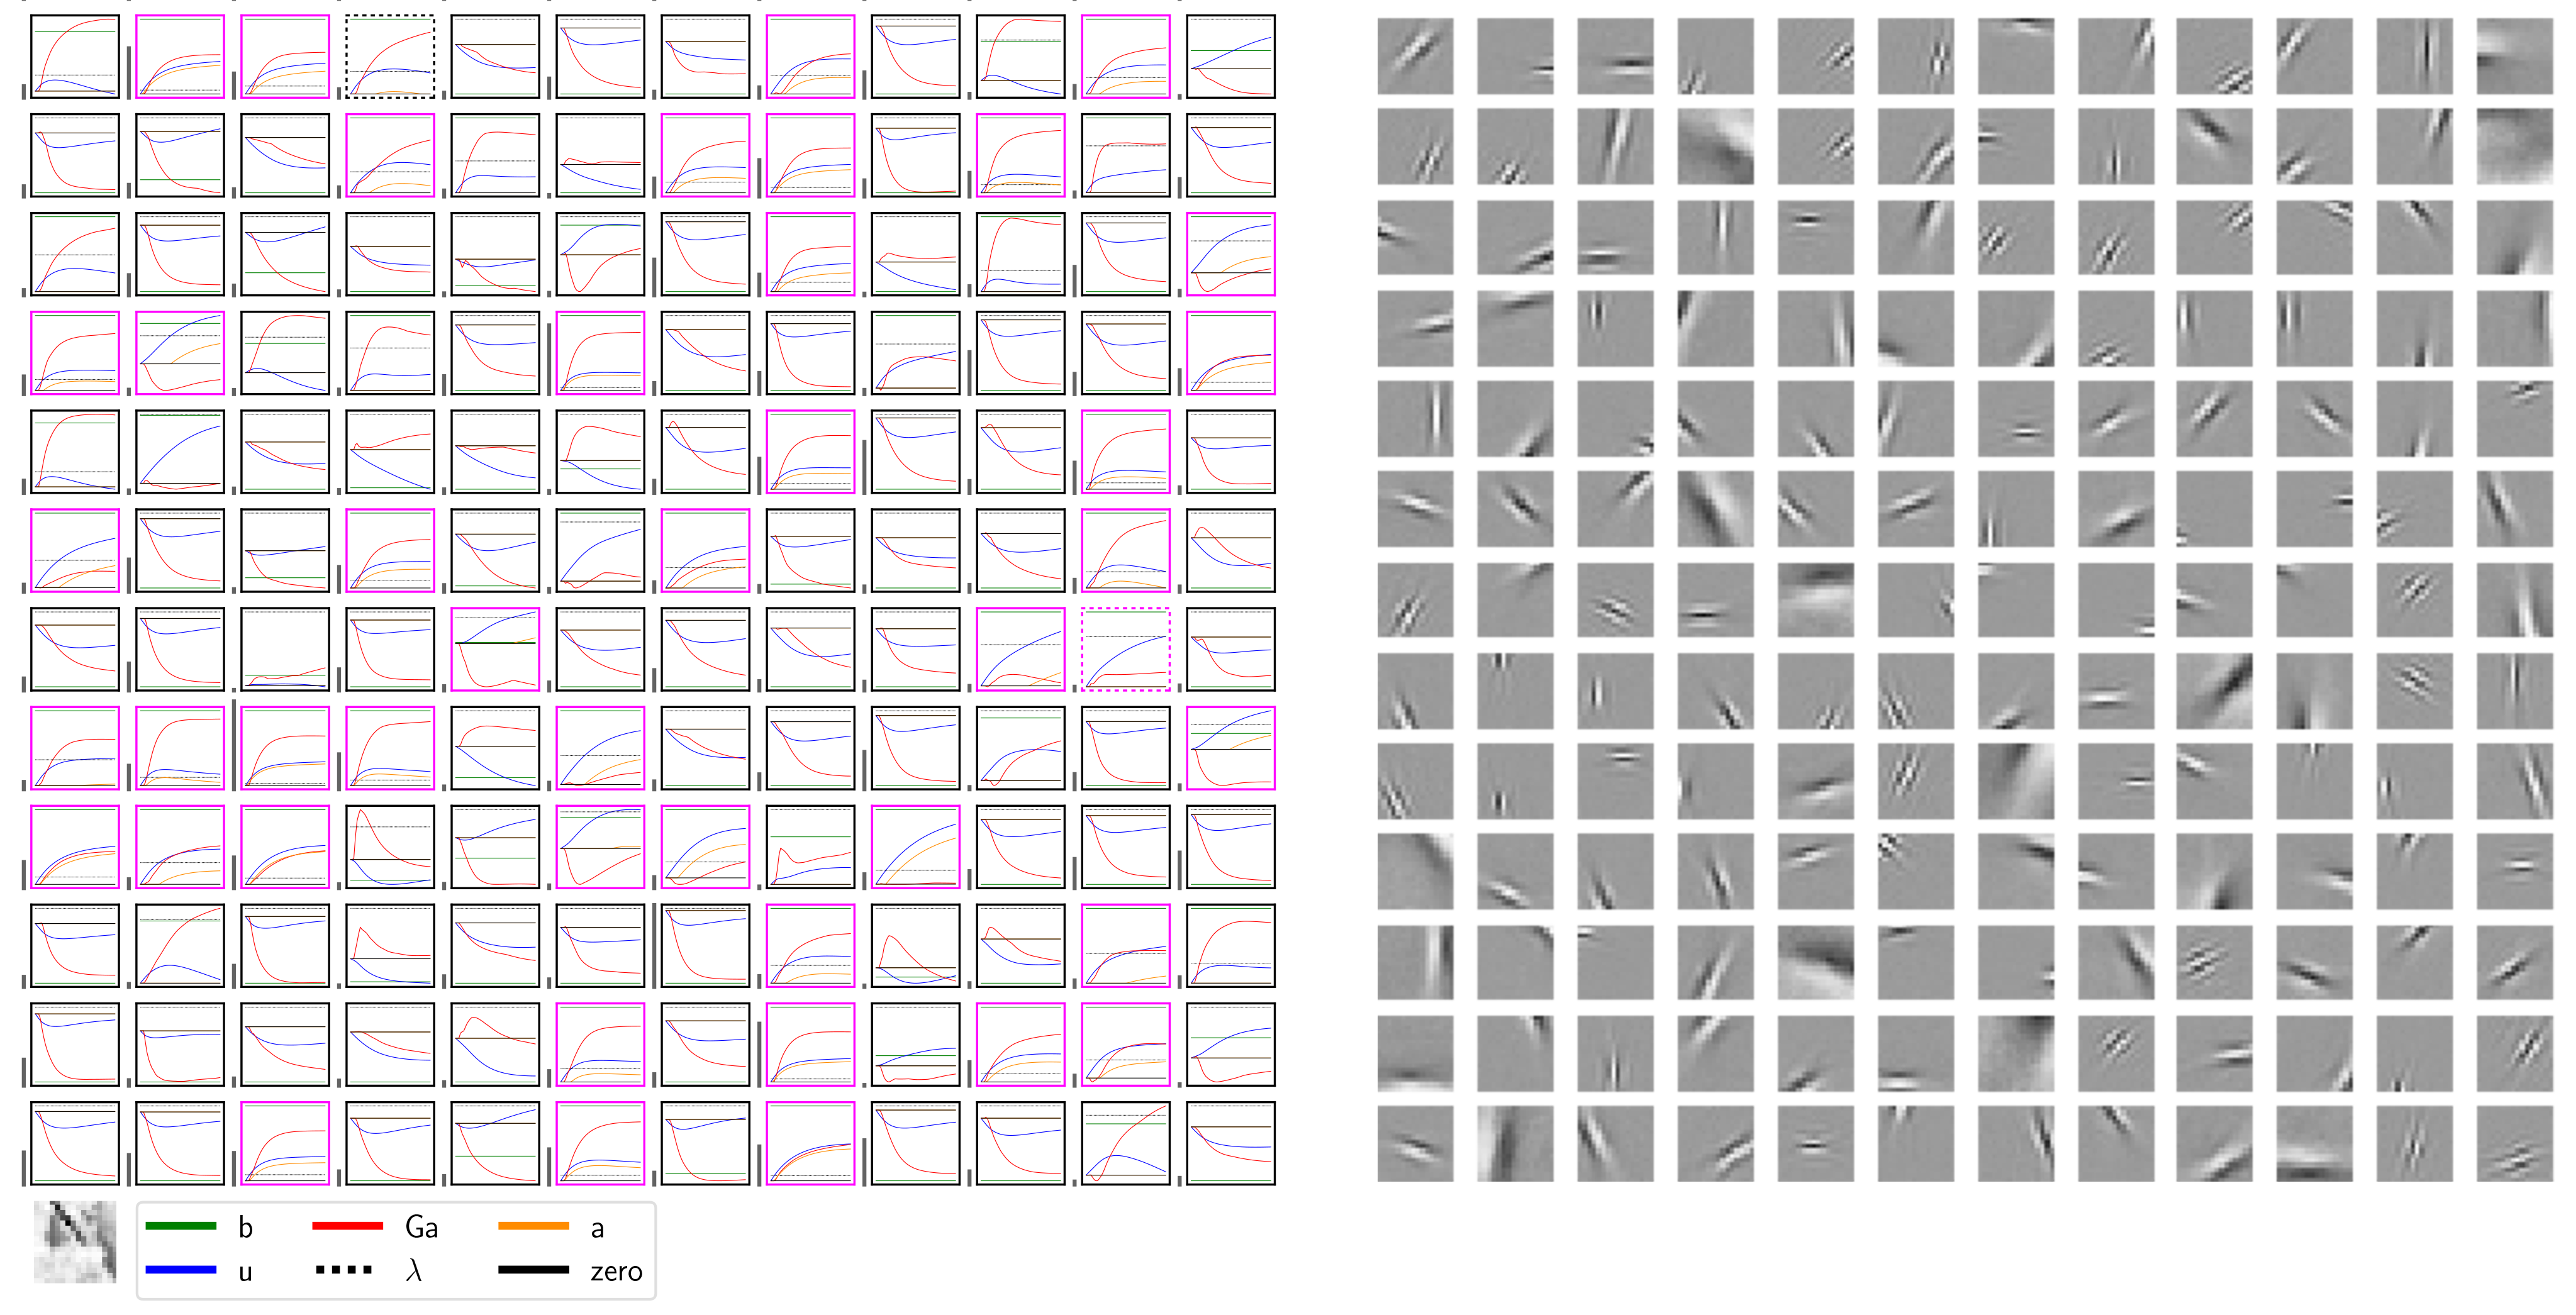
\includegraphics[width=\textwidth]{figures/lca_inference_traces.png}
    \caption{\textbf{Individual trace dynamics for LCA neurons.} Shown are input and output traces for a subset out of 768 LCA neurons during inference. The input image is in the bottom left. Each trace plot has a corresponding weight, shown in figure \ref{fig:ch2_lca_inference_weights}.  The lines in the trace plot represent terms from equation \eqref{eq:ch2_lca_deda_simple}, as indicated in the legend. The grey bars on the left of each trace plot indicate relative scale of the vertical axis. A magenta boundary indicates that the neuron was active at the end of the inference period, and a black boundary indicates otherwise. A dotted boundary indicates that it became active or inactive in the last 20 percent of the inference process.}
    \label{fig:ch2_lca_inference_traces}
\end{figure}
\chapter{Hierarchical LCA}

\section{Related hierarchical sparse coding models}\label{sec:ch3_related_models}
Ultimately, we aim to build a hierarchical general representation of natural scenes. A hierarchical model of natural scenes should produce a general representation of input data that spans all layers. The bottom of the hierarchy contains information about the details of the scene, and as one ascends the hierarchy, one should see a more general, abstract description. Information should move up the hierarchy in the form of inference and down the hierarchy as expectations or priors. Resolving ambiguities at the top should be easier as there are more regularities and there is more context. These should help inform inference in lower layers to resolve more difficult ambiguities about details of the scene.

Broadly speaking, there have been many hierarchical unsupervised learning architectures in the literature. Here we will highlight work that is particularly relevant considering the goals of the previous paragraph. Lee and Mumford \citeyearpar{lee2003hierarchical} propose a model that comes very close to what was described in the previous paragraph. They simplify the model by forcing each layer to only receive input from the layer below & above, as in a Markov chain. Expectations are propagated down to alter priors of lower layers in a dynamic, context-sensitive manner. Feedback connections influence the inference process, causing a layer to converge on a solution that fits the expectations above. Although they use dynamic sampling algorithms to represent Bayesian inference, we believe it is possible to construct a version that is true to the theory and uses sparse coding as a core computational framework. We identify this as an exciting area of future research. Karklin and Lewicki \citeyearpar{karklin2003learning} propose a hierarchical probabilistic model that is an extension of the ICA model. They start with learning a complete orthogonal basis with ICA, and then learn ``variance bases'' that model higher-order structure in images. Their model produces a hierarchical sparse distributed code of natural scenes, although they do not perform inference but instead directly compute first layer activations in a feed-forward architecture. They are able to learn to represent higher-order structure such as elongated edges with a nonlinear inference process because the joint coefficient distribution is replaced with a hierarchical prior. An exciting extension of this work would be to extend the LCA model to include their probabilistic model. The variances learned in the second layer can then be used to guide LCA inference. Shan and Cottrell \citeyearpar{shan2013efficient}  demonstrate a hierarchical model by alternating a PCA variant and ICA transforms. They learn representations that resemble those of other hierarchical models by using PCA to reduce the dimensionality of ICA outputs and then learning an overcomplete ICA \parencite{le2011ica} representation on the PCA activations. Although their model is not derived from a probabilistic framework and is linear in the activations, it is a promising proof of concept for a framework that alternates dimensionality reduction and expansion to learn higher-order structure from natural images. Cadieu and Olshausen \citeyearpar{cadieu2008learning} propose a two-layer sparse coding network that explicitly disentangles form and motion in the second layer when trained on video input. The first layer is a sparse coding model that is trained with complex valued dictionary elements. They then factorize the first layer output into two sets of second layer inputs that encode the time-derivative of the amplitude and phase components to explicitly separate form and motion, respectively. The second layer units also perform sparse coding on the logarithm of factorized quantities from the first layer. They demonstrate that form selective neurons develop invariance properties from the time-varying signal. A convolutional LCA variant called the Deconvolutional Competitive Algorithm (DCA) is proposed in \parencite{paiton2015deconvolutional} that deconstructs images into a three-layer hierarchical code. The network performs inference in all three layers simultaneously, and all three layers compete to reconstruct the image. By configuring the strides and patch sizes appropriately, the network was designed such that each layer contributes a different degree of detail. The lowest layer reconstructed high spatial frequency, grayscale details while the highest layer reconstructed low spatial frequency and color information. The generative process is linear and therefore could be represented with a single dictionary. Ideally, we would like the generative process to be able to account for the non-linear structure in images. The sparse manifold transform was proposed by \parencite{chen2018sparse}, which is an extendable hierarchical sparse coding network that models the underlying manifold structure of time-varying natural scenes. The model combines dimensionality expansion using sparse coding and reduction using manifold embedding. The transform is also invertible via a non-linear generative process, such that linear translations in the embedded space result in non-linear transformations in the image space. The learned dimensionality reduction step can be thought of as an alternative to pooling operations commonly found in deep learning architectures.

%\subsection{PCA dimensionality reduction to learn second layer units}
%Hyvarinen & Hoyer strong PCA work; my project implementing this with LCA


\section{Weakly-Supervised Feature Learning}\label{sec:ch3_weak_supervised_learning}

\subsection{Introduction}
We evolved a visual sense to allow us to understand the external causes of incident light. The sensor modality is not designed to construct a veridical representation of the world \parencite{gollisch2010eye}. Instead, it is designed to allow us to identify objects of significance and act upon them. Our visual system is intimately connected with the statistics of light as it propagates through our natural world. These statistics have been analyzed extensively by scientists exploring images and videos of natural scenes (see chapter \ref{ch:intro}. The sparse coding model represents an attempt to build on the knowledge gained from studying the statistics of natural scenes to better understand our visual system. In the field of visual unsupervised machine learning, a cornucopia of models have been proposed to learn the statistics of natural scenes without human labels, or ``supervision'' \parencite{baldi2012autoencoders, bengio2012unsupervised, goodfellow2016deep}. It is important to recognize that the unsupervised objective function of most of these models does in fact ask for a veridical representation of the inputs, without any real consideration for other ecological significance for the latent code produced. None the less, when combine with a family of constraints that include minimum entropy, maximum compression, and minimal energy expenditure, autoencoder models can exhibit interesting properties that are also found in biological vision systems. In this chapter, we consider the LCA as an autoencoder. Like an autoencoder, the LCA receives inputs, transforms them into a latent code, and produces reconstructions. We are interested in understanding how useful LCA can be for the machine learning field. One way to assess this is to look at semi-supervised learning. Here the objective is the same as for supervised learning, where we want to associate images with some predetermined category label. However, the catch is that many of the training images do not have ground truth labels assigned to them. A fully supervised model would not be able to use these, and would suffer from limited training examples. Here we show that LCA can be used as an agent to improve semi-supervised learning results. We also demonstrate how an alternate objective, like labeling objects in the world, can be used in the LCA dynamics to modify inference and dictionary learning.

\subsection{Weakly-supervised learning}
%[https://docs.google.com/presentation/d/1Dy_Dy1uSnLC3FEWXczgdKGxSejRUYQmfHnwPtY5LA8Y/edit#slide=id.g12e96bb738_0_271]
%[https://docs.google.com/presentation/d/1CcFmB1AUIEWU_rKtIaiRM79QGMetjYhnjKfv58hDD8Y/edit#slide=id.g19049d0ee0_0_22]
%[https://docs.google.com/document/d/13IzufcIS9M9HTCKsQGPSWmCB7lbm4axBAVbGeEml-ks/edit?usp=sharing]
%[https://docs.google.com/presentation/d/1bW__4dYIlrrbiV55Y1WdKcI_jxYqCSPXVpQjnumrDfo/edit#slide=id.g13eab2f708_0_83 slide 11]

Human labels are extremely expensive and often biased. A learning paradigm that avoids this process is unsupervised learning, but it is not directly applicable to the machine learning task of assigning labels to, or categorizing, data. Weakly-supervised learning is a sub-field that aims to combine the benefits of unsupervised and supervised learning. An ideal model should learn to categorize (e.g. cluster) data without ground-truth labels while still maintaining a faithful representation. As we demonstrate in chapter \ref{ch:iso}, sparse coding produces a code that is both descriptive and faithful to the image content. Here, we wish to modify the sparse coding model to utilize limited label information about an input scene.

\subsubsection{Features learned in unsupervised frameworks match those learned in supervised frameworks}
The Discriminative Recurrent Sparse Auto-Encoder (DrSAE, \cite{rolfe2013discriminative}) behaves similarly to sparse coding and has been shown to be successful at semi-supervised learning. Unlike LCA, the encoder, decoder, and lateral connectivity weights of DrSAE are unconstrained and trained independently. However, when trained on the MNIST dataset \parencite{lecun1998mnist}, the DrSAE learns weights that closely match what we impose for sparse coding. That is, the decoder weights have high correspondence to the transpose of the encoder weights and the lateral connectivity weights have high correspondence with the Gramian of the encoder weights. Additionally, when semi-supervised training is performed, the model learns an emergent hierarchical architecture. Figure \ref{fig:ch3_lenet_lca_drsae_weights} shows that the features learned by the unsupervised LCA and DrSAE models have a high degree of structural similarity to those learned by a supervised model \parencite{lecun1998gradient}.

\begin{figure}\label{fig:ch3_lenet_lca_drsae_weights}
    \centering
    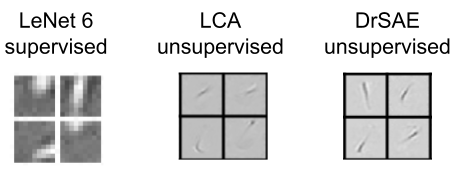
\includegraphics[width=\textwidth]{figures/lenet_lca_drsae_weights.png}
    \caption{\textbf{Unsupervised learning leads to similar features.} The features learned from unsupervised training on MNIST using LCA \parencite{rozell2008sparse} and DrSAE \parencite{rolfe2013discriminative} have similar structure to those learned using the supervised LeNet model \parencite{lecun1998gradient}}
\end{figure}

The DrSAE model was also extended to a semi-supervised learning framework. Given their success, we constructed a similar framework with LCA. The LCA dynamics are derived from a principled energy function, so we were able to extend the framework by adding semi-supervised loss terms to the energy function. Typically in sparse coding the sparsity enforcing term is applied uniformly, penalizing all nodes. Instead of the prior limiting the total activation, we want the prior to encourage some nodes to be active based on expectations propagated down from higher layers. These higher layers could be focused on grouping inputs into similar categories. We will incorporate a new loss function to encourage unsupervised clustering. This loss function minimizes the output entropy per image, but maximizes it per batch. The intuition is that minimizing entropy per image will force the network to place the image into a category, since the number of output nodes is small (e.g. ~10 for MNIST). Maximizing the entropy across batches is intended to prevent the network from placing all images into a single category, assuming there is an approximately even distribution of classes in a given batch. We will add a second layer on top of the LCA network and enforce a categorical cost. The cost is cross-entropy when there is a label or the combined entropy terms described earlier when there is not. Taking the derivative of this new cost with respect to a neuron will give us a new update rule for inference.

Our proposed model is capable of weakly-supervised learning, where only a small percentage of data examples have corresponding labels. We used the model for categorizing novel inputs using a heavily reduced set of labeled examples. Typical solutions to this problem utilize a combination of supervised and unsupervised learning objectives. The supervised objective aims to build an association between a given input and label, such that similar inputs receive the same label. The unsupervised learning objective aims to preserve a faithful representation of the input, such that the input data can be reconstructed directly from the network activations. In a typical scheme, the supervised objective is used when labels are available and the unsupervised objective is used when they are absent. In addition to these two classic objectives, we have added an additional unsupervised objective that encourages the network to confidently group the inputs into categories. In the unsupervised case we do not have a training label to verify the network’s categorization, so we instead encourage the network to be as confident as possible about the category it has assigned to the input, regardless of the accuracy of the categorization. This additional objective improves the network’s ability to categorize inputs, which is typically absent from unsupervised learning.


\subsubsection{LCA with feedback model description}
A traditional deep network layer produces an output by filtering input data through a linear weight matrix and a nonlinear thresholding function. The thresholded output is then passed to the next layer in the hierarchy. Dimension-reducing nonlinearities, such as max-pooling are also often included between layers to increase network invariance to label-preserving variations in the data as well as to prevent combinatorially increasing layer size with depth. This process continues until, ultimately, a probability distribution over possible categories is produced as the final layer’s output. For static data classification, such as image labeling, most deployed state-of-the-art networks are feedforward in that information strictly flows in one direction through the network. Additionally, the layers themselves do not demonstrate a dynamical response to the input. In our alternative approach, each layer performs a dynamical non-linear computation on the input. The first layer is an LCA layer that incorporates lateral connectivity between neurons to enforce competition, creating a descriptive, distributed sparse code of the input data. This code is produced in a recurrent fashion, where the network dynamics evolve through time to a converged representation of the input. Additionally, each LCA neuron receives input from the layer above that alters the dynamics in a context-dependent way. The resulting network representation is hierarchical and faithful to the input, such that the data can be directly reconstructed from the neuron activation values. Within-layer competition and top-down feedback encourage the network to produce a maximally descriptive code that is context-aware. The semi-supervised nature of the model will allow us to leverage raw data without the need for expensive human labeling.

For the LCA with feedback (LCAF) model, we will add an additional classification layer on top of the LCA model, as illustrated in figure \ref{fig:ch3_mlp_lcaf_architectures}.  The network minimizes one of two different energy functions, depending on whether there input image has a provided label. In the case that there is a label, the energy function is the same as was used in equation \ref{eq:ch2_sparse_energy}, with the addition a the cross-entropy loss:

\begin{equation}\label{eq:ch3_lcaf_supervised_energy}
         E =
        \overbrace{ \tfrac{1}{2} \| s - \hat{s} \|_{2}^{2} }^\text{Preserve Information} +
        \overbrace{ \lambda \sum\limits_{i=1}^{M}C(a_{i}) }^\text{Limit Activations} -
        \overbrace{ \alpha \sum\limits_{j=1}^{K} y_{j}log(\hat{y_{j}})}^\text{Cross-Entropy Cost},
\end{equation}

\noindent where $K$ is the number of categories, $\alpha$ is a tunable trade-off parameter, $y_{j}$ is a ground-truth one-hot label, and $\hat{y_{j}} = \frac{e^{-Wa_{j}}}{\sum_{n}e^{-Wa_{n}}}$ is the softmax output of the classification layer. When a label is not present, we swap out the cross entropy cost with an entropy cost. We want our model to have high confidence (low entropy) per image and high entropy across batch (because we are assuming the categories are evenly distributed). We do this by defining two entropy terms. The first computes the entropy per image by summing across the neuron indices:

\begin{align}\label{eq:ch3_lcaf_q_dist}
\begin{split}
  Q_{i,l} &= \frac{e^{-\gamma \hat{y}_{i,l}}}{\sum\limits_{k=1}^{K}e^{-\gamma \hat{y}_{k,l}}} \\
  H^{\text{neuron}}_{l} &= -\sum_{i}Q_{i,l}\log Q_{i,l}.
 \end{split}
\end{align}

The second term computes the batch entropy by summing across the batch dimension:

\begin{align}\label{eq:ch3_lcaf_p_dist}
\begin{split}
  P_{i,l} &= \frac{e^{-\gamma \hat{y}_{i,l}}}{\sum\limits_{b=1}^{B} e^{-\gamma \hat{y}_{i,b}}} \\
  H^{\text{batch}}_{i} &= -\sum_{l}P_{i,l}\log P_{i,l},
 \end{split}
\end{align}

\noindent where $B$ is the batch size. Now we can combine these terms for our unsupervised entropy loss:

\begin{equation}\label{eq:ch3_lcaf_unsupervised_energy}
         E =
        \overbrace{ \tfrac{1}{2} \| s - \hat{s} \|_{2}^{2} }^\text{Preserve Information} +
        \overbrace{ \lambda \sum\limits_{i=1}^{M}C(a_{i}) }^\text{Limit Activations} +
        \overbrace{ \alpha_{1} \sum\limits_{l=1}^{K} H^{\text{neuron}}_{l} - \alpha_{2} \sum\limits_{i=1}^{B}H^{\text{batch}}_{i}}^\text{Entropy Cost},
\end{equation}

\noindent where $\alpha_{1}$ and $\alpha_{2}$ are tunable loss trade-off parameters. Our LCA inference equation follows the same derivation from equation \ref{eq:ch2_lca_deda_simple}, with an added term computed from the derivative of the entropy or cross-entropy costs with respect to the activity vector, $a$.

%TODO: add lca update rule (https://docs.google.com/presentation/d/1Dy_Dy1uSnLC3FEWXczgdKGxSejRUYQmfHnwPtY5LA8Y/edit#slide=id.g12e96bb738_0_211 for cross-entropy)

\begin{figure}\label{fig:ch3_mlp_lcaf_architectures}
    \centering
    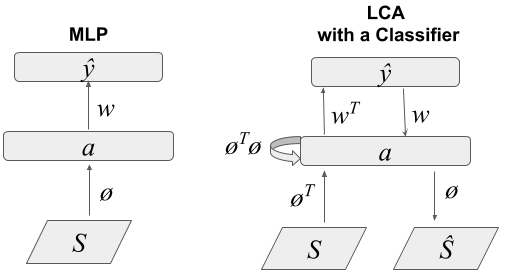
\includegraphics[width=0.5\textwidth]{figures/mlp_lcaf_architectures.png}
    \caption{\textbf{Training a classifier on LCA outputs.} We propose a two-layer LCA architecture that learns a set of weights using a semi-supervised objective in the second layer. We compare this against a standard 2-layer MLP architecture.}
\end{figure}

\subsection{Experiments on MNIST dataset}
Our fist experiment is to verify that the classifier is able to train using sparse codes as input. The following table gives the MNIST test accuracy using a fully supervised label set. The LCA model was pre-trained on MNIST without labels and then a single layer classifier was trained on the activity vector, $a$.

\begin{table}[]
\begin{tabular}{lllll}
 & \textbf{MLP} & \textbf{\begin{tabular}[c]{@{}l@{}}MLP with\\ random $\Phi$\end{tabular}} & \textbf{\begin{tabular}[c]{@{}l@{}}MLP with\\ LCA $\Phi$\end{tabular}} & \textbf{\begin{tabular}[c]{@{}l@{}}LCA with\\ classifier\end{tabular}} \\ \cline{2-5} 
\multicolumn{1}{l|}{\textbf{Test Error}} & \multicolumn{1}{l|}{411} & \multicolumn{1}{l|}{2979} & \multicolumn{1}{l|}{1723} & \multicolumn{1}{l|}{331} \\ \cline{2-5} 
\multicolumn{1}{l|}{\textbf{Test Accuracy}} & \multicolumn{1}{l|}{95.89\%} & \multicolumn{1}{l|}{70.21\%} & \multicolumn{1}{l|}{82.77\%} & \multicolumn{1}{l|}{96.69\%} \\ \cline{2-5} 
\end{tabular}
\caption{\textbf{LCA helps with MNIST classification.} This table shows that a single layer classifier trained on LCA encodings of the MNIST digit dataset outperforms a two layer classifier trained directly on MNIST pixels. The first column is the results for a two-layer classically trained MLP. The second is the same, except that the first layer weights were frozen with random initialization. The third had the first layer weights frozen to those that were trained with LCA, but did not utilize sparse inference. The final column is the results for a single-layer classifier trained on the LCA activations.}
\label{tab:ch3_mnist_accuracy}
\end{table}

Next we modified the MNIST dataset such that a varying percentage of the labels are removed to test our network’s ability to generalize and label unseen digit images. In table \ref{tab:ch3_restricted_mnist_accuracy}, we show that adding the supervised cross-entropy feedback to sparse inference had little effect on the limited label regime. However, combining the supervised cross-entropy feedback with the unsupervised entropy feedback resulted in an improved score with very few labeled examples. We note that these scores were not cross-validated, and therefore we cannot assign confidence scores to the accuracy reported. The error rates found from previous studies were 0.1\%, 1\%, and 5\% for 50000, 100, and 20 labeled examples respectively \parencite{rasmus2015semi}.

\begin{table}[]
\begin{tabular}{llll}
\multicolumn{1}{c}{\textbf{\begin{tabular}[c]{@{}c@{}}Number of labeled\\ training examples\end{tabular}}} & \multicolumn{1}{c}{\textbf{LCA}} & \multicolumn{1}{c}{\textbf{\begin{tabular}[c]{@{}c@{}}LCAF\\ sup only\end{tabular}}} & \multicolumn{1}{c}{\textbf{\begin{tabular}[c]{@{}c@{}}LCAF\\ sup and unsup\end{tabular}}} \\ \cline{2-4} 
\multicolumn{1}{l|}{\textbf{50,000}} & \multicolumn{1}{l|}{96\%} & \multicolumn{1}{l|}{96\%} & \multicolumn{1}{l|}{96\%} \\ \cline{2-4} 
\multicolumn{1}{l|}{\textbf{100}} & \multicolumn{1}{l|}{68\%} & \multicolumn{1}{l|}{67\%} & \multicolumn{1}{l|}{65\%} \\ \cline{2-4} 
\multicolumn{1}{l|}{\textbf{20}} & \multicolumn{1}{l|}{33\%} & \multicolumn{1}{l|}{33\%} & \multicolumn{1}{l|}{38\%} \\ \cline{2-4} 
\end{tabular}
\caption{\textbf{Feedback helps with MNIST classification.} We compare the LCA with classifier model against two variants: One with strictly supervised feedback (middle column) and another with supervised and unsupervised feedback (right column). Although the feedback does not appear to help when there are a large number of labeled examples, it does show a positive effect when the number of labeled examples is restricted.}
\label{tab:ch3_restricted_mnist_accuracy}
\end{table}

To test whether the unsupervised feedback term gave a meaningful signal, we measured the distances among sparse codes produced without feedback, with supervised feedback, and with unsupervised feedback. Figure \ref{fig:ch3_feedback_code_distances} shows that the Hamming distance between codes produced with either form of feedback are smaller than the distance from a code produced with feedback to one produced without feedback. This tells us that the feedback itself changes the code produced, and also that the unsupervised feedback produces a code that is similar to the supervised feedback code, which suggests that the unsupervised feedback is a good proxy for the supervised signal.

\begin{figure}
    \centering
    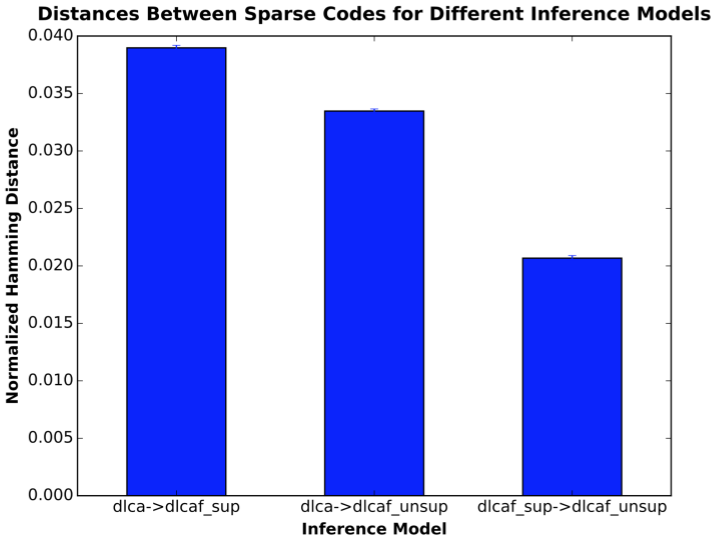
\includegraphics[width=0.5\textwidth]{figures/feedback_code_distances.png}
    \caption{\textbf{Unsupervised feedback during LCA inference produces similar codes to supervised feedback.} We measure the number of neurons that crossed their activation threshold (from active to inactive or vice versa) in terms of a Hamming distance. The distances between the codes produced without feedback and with either form of feedback (left two bars) are larger than the distance between the codes produced with supervised and unsupervised feedback (right bar). This tells us that the unsupervised entropy feedback produces a meaningful signal that is similar to that produced by supervised cross-entropy feedback. The bars height indicates mean hamming distance for 100 images and error bars indicate standard error of the mean.}
    \label{fig:ch3_feedback_code_distances}
\end{figure}

We also tested the weights learned with and without feedback during inference. In this experiment, the dictionary update rule is the same as was described in equation \ref{eq:ch2_phi_update}, but the sparse inference process was modified. Figure \ref{fig:ch3_feedback_nofeedback_features} shows that the feedback process influences the first layer weights learned to produce more prototypical digits. Additionally, the first layer neurons that are most strongly connected to a specific second layer classification neuron have a higher degree of correspondence to the classification category when feedback was used during inference.

\begin{figure}\label{fig:ch3_feedback_nofeedback_features}
    \centering
    \begin{subfigure}[b]{0.5\textwidth}\label{fig:ch3_nofeedback_features}
      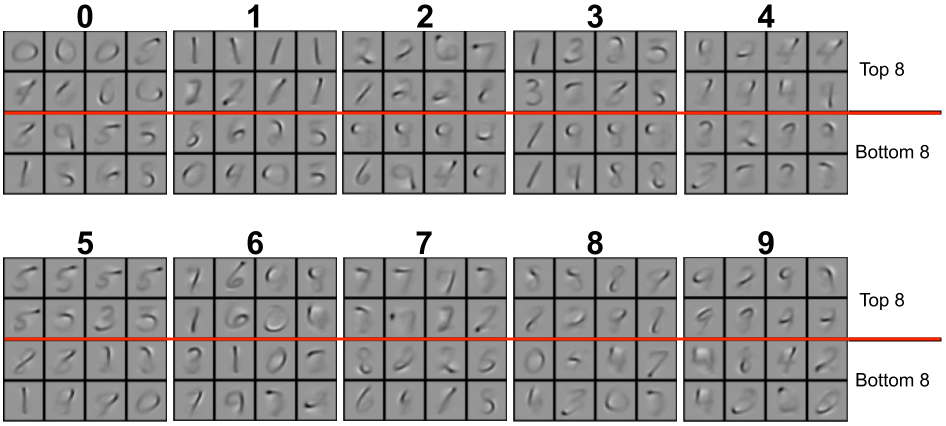
\includegraphics[width=\textwidth]{figures/lca_nofeedback_classifier_features.png}
      \caption{Without feedback}
    \end{subfigure}
    \begin{subfigure}[b]{0.5\textwidth}\label{fig:ch3_feedback_features}
      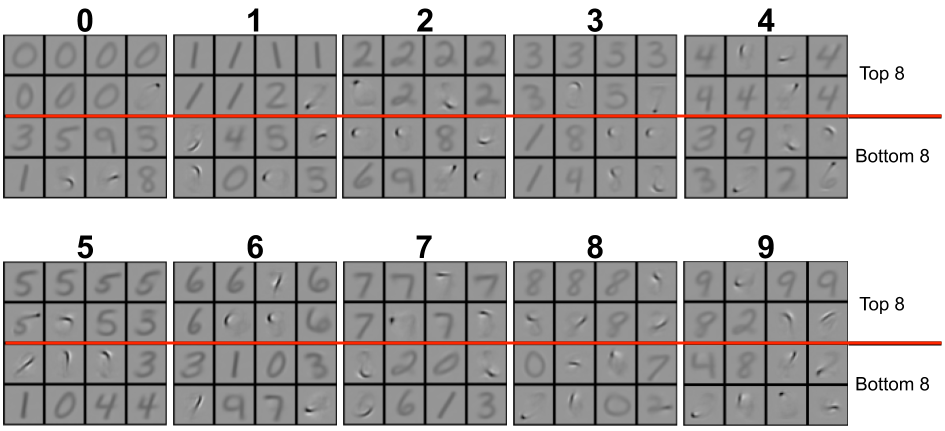
\includegraphics[width=\textwidth]{figures/lca_feedback_classifier_features.png}
      \caption{With supervised feedback}
    \end{subfigure}
    \caption{\textbf{The weights learned by the LCA classifier are affected by the supervised feedback signal.} The subfigures show the basis functions, $\Phi$, for the top and bottom strongest connected first layer neurons to each classification output neuron. (a) Inference was performed with supervised feedback. (b) Inference was performed without feedback. Each 4x4 grid corresponds to a particular classification label. Images above the red line are the basis functions for the 8 neurons that are most strongly connected to the given classification neuron and below the red line are the bottom 8. The basis functions themselves change with feedback, and the structure of the top connected basis functions is better matched to the digit label when feedback is used.}
\end{figure}

\subsection{Conclusion}
There is a strong need for statistical models to learn from data without human curated labels because of the considerable expense of generating such labels and to avoid the unintended biases that human labeling introduces. However, most deep neural networks - the gold standard in modern machine learning - are trained in a supervised manner and are predicated on a narrowly specified task, such as labeling objects in images or videos. We propose a semi-supervised deep network to learn a hierarchical representation of visual data with or without corresponding labels. Instead of a narrowly specified task, the primary objective of our model is constructing a general, hierarchical and efficient code of the data that can be applied to a myriad of different tasks. This section showcased a promising research direction of using supervised and unsupervised entropy signals to direct LCA inference. Much more work needs to be done to investigate how feedback is influencing inference and learning as well as making comparisons to alternative methods.


\section{Subspace LCA}\label{sec:ch3_subspace_lca}
\subsection{Introduction}
We describe an extension to the LCA model that produces invariant representations of its inputs. The model is similar to the Independent Subspace Analysis described in \parencite{hyvarinen2000emergence}, but differs in several key ways. First, the LCA model allows for the first layer representation to be overcomplete, which produces a more efficient representation (see \parencite{lewicki2000learning} and chapter \ref{ch:iso}). Second, the first layer encoding process is non-linear, which gives the neurons a higher degree of nonlinearity (chapter \ref{ch:iso}) and also improves efficiency (section \ref{sec:ch2_alternative_image_coding_models}).

\subsection{Model description}
The subspace LCA follows a similar derivation to the LCA (section \ref{sec:ch2_lca}). Like the LCA, it learns a set of weights to efficiently describe natural signals, although in this variant we constraint the weights to be grouped with the group size set as a hyper-parameter. We start with the same generative framework as in sparse coding:

\begin{equation} \label{eq:ch3_slcagenerative_model}
    s = \Phi a + \varepsilon.
\end{equation}

We will constrain our activations (and therefore weights) to non-overlapping groups that have an amplitude, $\sigma$:

\begin{align}\label{eq:ch3_a_decomp}
\begin{split}
  \sigma_{i} = ||a_{i}||_{2} = \sqrt{\sum_{j\in I}a^{2}_{ij}},
\end{split}
\end{align}

\noindent where $i$ indexes the group and $j \in I$ indexes the neuron within the group. The group amplitude is equivalent for many combinations of $a_{j \in I}$. Each of these equal combinations can be thought of as a direction of a vector in the activity space. We can formalize this with a unit-length direction vector, $z$, that has the same number of elements as our activity vector:

\begin{align}\label{eq:ch3_z_def}
\begin{split}
  z_{ik} = \frac{a_ik}{\sigma_{i}}.
\end{split}
\end{align}

We can now define a new energy function in these terms. We also add a regularization term that pressures the within-group weights to be orthogonal, which prevents the pathological solution of within-group neurons learning to have identical weights:

\begin{equation}\label{eq:ch3_subspace_lca_energy}
    E = \frac{1}{2}\sum_{p}\left[s_{p} - \sum_{ij}\sigma_{i}z_{ij}\Phi_{ijp}\right]^{2} + \lambda \sum_{i}\sigma_{i} + \alpha \sum_{ij}\left|\sum_{p} \Phi_{ijp}\Phi_{ijp} - \mathbf{I}_{L} \right|,
\end{equation}

\noindent where $\alpha$ is a trade-off multiplier, $\mathbf{I}_{L}$ is the $L \times L$ identity matrix, and $L$ is the number of neurons in a group. Following the LCA derivation in section \ref{sec:ch2_lca}, we will next take the derivative of the energy with respect to a neuron's activity:

\begin{equation}\label{eq:ch3_subspace_deda}
    -\frac{\partial E}{\partial a_{ik}} = \sum_{p}s_{p}\phi_{ikp} - \sum_{lm}G_{iklm}a_{lm} - \lambda \frac{\partial ||a_{i}||^{2}}{\partial a_{ik}}.
\end{equation}

We can rewrite the last term in the above equation as our direction vector:

\begin{align}\label{eq:ch3_subspace_deda_to_z}
\begin{split}
    \frac{\partial ||a_{i}||^{2}}{\partial a_{ik}} &= \frac{1}{2}\left(\sigma_{i}^{2}\right)^{-\tfrac{1}{2}}2a_{ik}\\
    &= \frac{a_{ik}}{\sigma_{i}}\\
    &= z_{ik}.
\end{split}
\end{align}

In parody with the LCA derivation, we group the self inhibition terms:

\begin{align}\label{eq:ch3_f_of_a}
\begin{split}
    f_{\lambda}(a_{ik}) &= a_{ik} + \lambda z_{ik}\\
    &= \overbrace{\sigma_{i}+\lambda}^\text{amplitude}\overbrace{z_{ik}}^\text{direction}\\
    &= a_{ik}(1 + \frac{\lambda}{\sigma_{i}}).
\end{split}
\end{align}

We again assign our membrane potential, $u$ as $f_{\lambda}(a_{ik})$:

\begin{equation}\label{eq:ch3_u_def}
  u_{ik} = f_{\lambda}(a_{ik}) = (\sigma_{i} + \lambda)z_{ik},
\end{equation}

which also gives us an alternative definition of the neuron angle, $z$:

\begin{equation}\label{eq:ch3_z_u_def}
   z_{ik} = \frac{u_{ik}}{\sigma_{i} + \lambda} = \frac{u_{ik}}{||a_{ik}||_{2} + \lambda}.
\end{equation}

The resulting membrane update rule is nearly identical to equation \ref{eq:ch2_u_dot_full}, except that the lateral competition term includes group assignments:

\begin{equation}\label{eq:ch3_subspace_u_dot_def}
   \tau \dot{u_{ik}} - u_{ik} = \sum_{p}s_{p}\phi_{ikp} \sum_{lm \ne ik}G_{iklm}a_{lm}.
\end{equation}

Finally, we define the output amplitude in terms of the group threshold:

\begin{equation}\label{eq:ch3_subspace_threshold_func}
    a_{ik} = T_{\lambda}(\sigma_{i}) = \left\{
    \begin{aligned}
        0,\;\; & \sigma_{i}\; \leq\; \lambda \\
        (\sigma_{i}-\lambda)z_{ik},\;\; &sigma_{i}\; >\; \lambda.
    \end{aligned}
    \right.
\end{equation}

This tells us that all within-group neurons become active when the group amplitude surpasses the threshold, $\lambda$. Figure \ref{fig:ch3_subspace_lca_graph} shows a diagram of the group model.

\begin{figure}\label{fig:ch3_subspace_lca_graph}
    \centering
    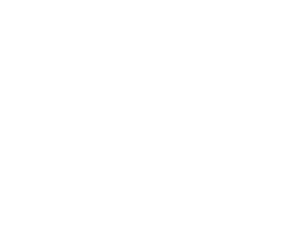
\includegraphics[width=0.5\textwidth]{figures/subspace_lca_graph.svg}
    \caption{\textbf{Subspace LCA}. Neurons are grouped such that they learn subspaces of co-active units. Once a group amplitude passes the threshold, all neurons in the group become active.}
\end{figure}

\subsection{Features learned}
When trained on natural images, the weights learn to tile orientations, spatial frequencies, and positions just like regular LCA. They also learn to have within-group similarities, such as equal orientation and position.

%TODO: redo weight images to be on the same scale
\begin{figure}\label{fig:ch3_subspace_lca_features}
    \centering
    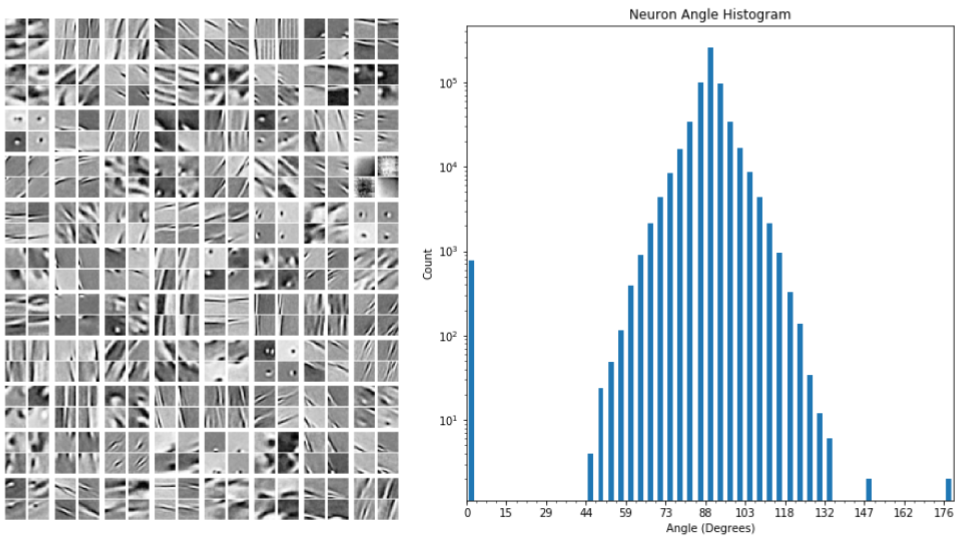
\includegraphics[width=\textwidth]{figures/subspace_lca_features.png}
    \caption{\textbf{Natural image features learned with subspace LCA}. Left) Subspace LCA learns features that have similar properties within group, but are different across groups. Right) The basis function angle histogram is very similar to that learned with LCA.}
\end{figure}

Interestingly, we show in figure \ref{fig:ch3_subspace_lca_mnist_features} that the group structure naturally separates digit classes when the model is trained unsupervised on the MNIST dataset. We believe this shows promise to use this model in a semi-supervised framework similar to that described in section \ref{sec:ch3_weak_supervised_learning}.

\begin{figure}\label{fig:ch3_subspace_lca_mnist_features}
    \centering
    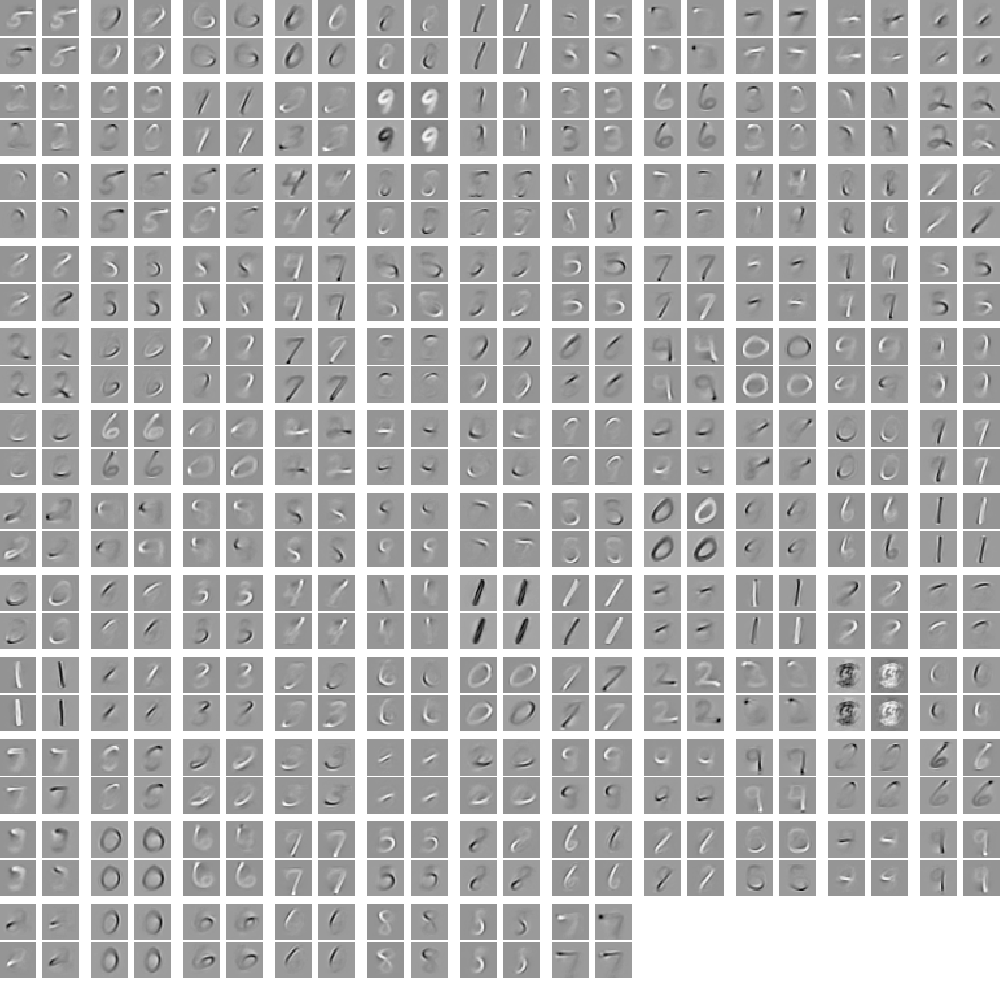
\includegraphics[width=\textwidth]{figures/subspace_lca_mnist_features.png}
    \caption{\textbf{MNIST features learned with subspace LCA}. The features learned with this model natural separate into digit categories, indicating that it might be a simple operation to assign images labels from the group amplitude representations.}
\end{figure}

\subsection{Conclusion}
In this section we demonstrate a novel extension of the LCA that learns statistical dependencies of sparse codes by grouping co-active elements into subspaces. Future work includes drawing comparisons to the Independent Subspace Analysis (ISA - \cite{hyvarinen2000emergence} and extending the model to a topographic version. Also, we believe this formulation can be extended to include ideas from dynamic routing \parencite{olshausen1993neurobiological}, where the $z$ variables ``steer'' the output representation.\label{ch:iso}
\chapter{Iso-Response Contours Provide a Geometric Interpretation of Neurons}

\section{Introduction}\label{sec:ch4_intro}
%* Theories for how/why attacks happen
%- cascading linearity (goodfellow et al. 2015)
%- excessive invariance
%- subspace view
%- classication boundary curvature view
%- ford et all adv examples & noise
%    * adv examples are the nearest test error
%    * although our model doesn't have better test error, we argue that the nearest point is more data-aligned.
%    * We should also test against distribution shift (fig 7, right from their paper)
%    
%* Defense methods
%- supplementing the dataset with adversarial examples
%- augmenting loss function with adv loss (madry)
%- preprocessing / denoising images (although this is difficult to do without heavily reducing model performance)
%
%* Models that have relevance to ours:
%- sun et al (sparse coding, although they are also obfuscating gradients)
%- marzi et al (sparsity, although they are also obfuscating gradients)
%- DARCCC (population nonlienarity?)
%* Find more papers that look at adversarial images compared to the image manifold \parencite{sun2018adversarial}.

Adversarial examples are a demonstration of an ANN’s inability to cope with a distributional shift from its training data \parencite{ford2019adversarial}. They represent a worst-case demonstration of this weakness, which is a general problem that all classification ANNs are susceptible to \parencite{hendrycks2018benchmarking}. We postulate that designing machine learning algorithms that are both accurate and robust to adversarial attacks requires a radical reformulation in how such algorithms are currently constructed. In particular, we propose to abandon a strict reliance on reducing classification loss (i.e. an exclusive focus on classification accuracy) and instead allow our models to undergo a period of unsupervised learning that mimics the cognitive development of biological nervous systems. Biological systems are robust to adversarial examples that affect deep networks. However, in time-limited regimes that result in predominantly feed-forward brain computation adversarial attacks have been shown to influence human decision making \parencite{elsayed2018adversarial}, suggesting that slower recurrent feedback loops aid in adversarial robustness. Furthermore, congruent with current theories for probabilistic inference in the brain \parencite{lee2003hierarchical}, we augment the standard ANN architecture with lateral connectivity and recurrence. We propose that, together, these innovations will improve the network’s specificity to signals that lie along the data manifold. We use adversarial attacks as a mechanism for understanding both traditional pointwise nonlinear ANNs and a population nonlinear alternative.

Adversarial attacks represent a recently discovered flaw in typical deep neural networks, where small targeted perturbations in the input space can cause large undesired changes in the output space. Although the discovery of adversarial examples in deep networks is relatively new, a fervor of research has produced a large body of literature on the subject and an understanding of these attacks has begun to emerge. In the pioneering work of Szegedy et al. \citeyearpar{szegedy2013intriguing}, they introduce the idea of ``adversarial attacks'' for deep networks and propose that a non-smooth decision boundary in classification networks produces adversarial ``pockets'' interspersed among dataset examples. They also suggest that adversarial images represent a counter-example to the hypothesis that deep networks are able to achieve local generalization to input space regions in the vicinity of training examples. Although this latter hypothesis has continued to hold, the presence of universal and transferable adversarial directions \parencite{moosavi2017universal} suggests that there are not adversarial pockets in the input manifold. The follow up work of Goodfellow et al. \citeyearpar{goodfellow2014explaining} make several proposals, some of which have been refuted \parencite{jetley2018friends}. However, we would like to emphasize two important arguments from their work: 1) they present evidence suggesting that the direction of perturbation is more important than the specific point in space (further refuting the ``pockets'' theory), and 2) the adversarial perturbations are highly aligned with the weight vectors of a model. The last of those observations has been explored in much more detail by Jetley et al. \citeyearpar{jetley2018friends}, who suggest that deep networks produce classification boundaries based on a small number of features that correspond to high curvature directions in the input space and that these high curvature directions are also the most effective adversarial directions. The works of Gilmer et al. \citeyearpar{gilmer2018adversarial} and Ford et al. \citeyearpar{ford2019adversarial} further expand on this idea by suggesting that adversarial attacks confined to the $l_{\infty}$ box represent the worst-case example of the model's inability to account for distributional shift generally. However, the works of Kos et al. \citeyearpar{ford2019adversarial} and Goodfellow et al. \citeyearpar{goodfellow2014explaining} demonstrate the ability to produce adversarial examples for pointwise-nonlinear generative models that have applications in image denoising, suggesting a more nuanced explanation of adversarial susceptibility. Recent work has also shown that nearly all proposed adversarial defense mechanisms fail in the face of more careful attacks \parencite{carlini2017towards, athalye2018obfuscated}.  For example, the recent defense method proposed by \parencite{sun2018adversarial} claims to produce an adversarially robust preprocessing step, although they use basis pursuit in their methods, which possibly achieves robustness through gradient obfuscation \parencite{athalye2018obfuscated}. However, their intuition that images should be forced onto the image manifold as a preprocessing step has great relevance to the work herein. It will always be possible to produce an image perturbation that results in a change in class label, or an alternate reconstruction. The academic fascination in the subject comes from observations of how small that perturbation needs to be and the (lack of) semantic content of the perturbation. Following the intuition provided in \parencite{ford2019adversarial}, successful defenses appear to require accomplishing one of two goals: 1) robustly denoising inputs to prevent distributional shift or 2) training deep networks to be more robust to worst-case distributional shift.

Inferring causes from natural signals is a challenging problem faced by biological vision systems. For artificial vision, the neural network community has largely tackled this problem using feedforward discriminative models. An alternative approach is to use generative models, in which the network must attempt to explain data in terms of an internal model of the world. In BNNs we see a preponderance of evidence that individual neurons are highly non-linear, recurrent, and laterally connected. The Locally Competitive Algorithm (LCA) \parencite{rozell2008sparse} is a generative sparse coding model that represents an example of how lateral inhibition can be derived from a well-defined computational objective. This network has been shown previously to exhibit a variety of non-linear receptive field effects \parencite{zhu2013visual}. Many of these effects can be explained using the model neuron’s iso-response contours - a common experimental method in neuroscience for determining stimulus combinations that result in equal activation from recorded neurons \parencite{golden2016conjectures}. In the brain, the atomic unit of computation is generally considered to be the neuron, but most deep learning research has eschewed the individual neuron, possibly obfuscating the connections between BNNs and ANNs. We propose to adopt the single-neuron iso-response analysis to better understand adversarial attacks on ANNs while varying degrees of biological realism.

To better understand how adversarial attacks differ for BNNs and ANNs, we compared feed-forward, pointwise nonlinear discriminative and generative network architectures against more biologically informed population nonlinear generative network architectures. Pointwise nonlinearities are the more traditional form of nonlinearities, as seen in nearly all deep neural network architectures. They are defined as nonlinearities that are a function of only a single neuron in a layer and include rectification, sigmoid, and hyperbolic tangent. Population nonlinearities represent the alternative class, where the nonlinearity output is a function of multiple neurons in a set. These include softmax, divisive normalization \parencite{carandini2012normalization, balle2016end} and the network nonlinearity present in sparse coding \parencite{rozell2008sparse, olshausen1997sparse}. In principle, generative models should not be as susceptible to adversarial attacks as discriminative models because they are trying to fit their internal model to the data as a ``sanity check'', which should not succeed for adversarial perturbations. One method by which generative models can perform such a sanity check is via recurrent maximum a-posteriori (MAP) inference. The LCA network uses population nonlinear interactions via lateral connectivity among neurons to facilitate this process, resulting in an ``explaining away'' effect commonly referenced in Bayesian inference literature \parencite{olshausen2013perception}.

Here, drawing from the architecture and function of brains, we propose that a network with lateral inhibitory connectivity in its hidden layer forces adversarial perturbation vectors to have angles that are more in line with data dimensions, producing more semantically meaningful perturbations. We develop an analytic argument to support this claim for untargeted adversarial attacks. Furthermore, we demonstrate by experiment that our method successfully improves robustness to adversarial attacks and more broadly distributional shift for a classifier trained on our model's outputs. The contribution of our work is a novel perspective for understanding adversarial attacks and population nonlinear networks. We also demonstrate that simple generative models can be used to improve a typical network’s defenses against adversarial attacks.

\section{Neuron response geometry explains adversarial robustness}\label{sec:ch4_neuron}
We propose to perform single neuron and population level analysis by extending the iso-response contour theory to be used as a lens to understand untargeted adversarial perturbations for individual neurons. Additionally, we have scaled up the iso-response analysis to models trained on images of handwritten digits (MNIST, \parencite{lecun1998mnist}) and natural scenes (CIFAR, \parencite{krizhevsky2009learning}). We show that the response geometry of LCA neurons predicts data-aligned perturbations when attacking the entire network, resulting in semantically meaningful adversarial attacks. We provide a theoretical argument to support this intuition by exploring the iso-response contours and orthogonal adversarial directions for individual neurons and give empirical evidence to further bolster the claims. 

Biological neurons are highly interconnected, both across and within layers. This interconnection gives rise to strong population nonlinear effects. However, nearly all work in neuron modeling uses pointwise nonlinearities due to the ease in interpretation and implementation. Work from \citeyearpar{golden2016conjectures} suggests a novel single-neuron analysis technique that allows us to increase the complexity of our neuron models without decreasing our understanding by looking at the neuron’s response geometry. We extend this technique to larger scale models that allows us to predict important properties about the model’s susceptibility to adversarial attacks. We then analyze the attacks themselves to demonstrate how the single-neuron analysis extends to networks. We conduct our preliminary experimentation on two types of networks: those with pointwise nonlinearities and those with population nonlinearities (figure \ref{fig:ch4_iso_contours}). Although there are many types of networks that fit into these two categories, we reserve comparative analysis among them to future work and focus this study on two specific instances: Feedforward Autoencoders (AEs) and the Locally Competitive Algorithm (LCA). We focus on the LCA as the population nonlinear network because it has been shown to exhibit many linear and nonlinear response properties that are well matched to what is observed in the brain \parencite{zhu2013visual, olshausen1997sparse}. The LCA was first proposed by Rozell et al. \citeyearpar{rozell2008sparse} to perform sparse coding. It is a generative network that uses MAP estimates of data likelihood to build an internal model. It can also be thought of as an auto-encoder with a single recurrent hidden layer. Details on these models can be found in section \ref{sec:ch4_comparison_models}.

\subsection{Adversarial examples are orthogonal to iso-response contours}
To better understand the difference between population and pointwise nonlinearities, we visualize the input-output maps of model neurons in the form of iso-response contours (figure \ref{fig:ch4_iso_contours}, see caption for more details). Golden et al. \citeyearpar{golden2016conjectures} used iso-response contours to explain several non-linear properties as well as variance/invariance properties for simple and complex cells. To construct the visualization, we consider a two-dimensional slice, or projection, in the high dimensional input space. We use each point (i.e. image) in the slice as input to the neuron model and bin the points according to the neuron's output amplitude (figure \ref{fig:ch4_iso_contours}). The iso-response contours of linear neurons are straight: any input perturbation that is orthogonal to the weight vector will result in equal activation. For pointwise nonlinearities, this remains true: because the nonlinearity is performed after a linear projection, the output must also produce straight iso-response contours. By contrast, for a population nonlinearity the gradient of the activation function with respect to a small perturbation in the input is a function of all other neurons in the layer. Thus, for a perturbation that is orthogonal to a target neuron, it is highly likely that an alternative neuron will have a non-orthogonal weight vector, which will result in a net change in all neuron outputs. Therefore, iso-response contours for population nonlinear neurons can be bent.

Adversarial examples are closely tied to neuron iso-response contours. While an iso-response contour represents a perturbation direction in stimulus space that produces no change in the output, an adversarial example is a perturbation direction that produces a maximal change in the output. Below, we present analytic arguments that these two response directions are orthogonal for individual neurons.

If we extend the work of Marzi et al. \citeyearpar{marzi2018sparsity} to include nonlinear functions, then we can define adversaries as seeking to maximize the following measure, $\Delta$, with respect to a perturbation, $e$:

\begin{align}\label{eq:ch4_adv_metric}
\begin{split}
    \max_{e} \Delta (s, s+e) = \max_{e} |f(s+e) - f(s)| \\
    s.t. \|e\|_{\infty} < \varepsilon,
\end{split}
\end{align}

where $f()$ can include a non-linear activation function, $s$ and $e$ are equal sized column vectors representing the data and perturbation, respectively, and $\varepsilon$ is some small scalar value. To solve this equation, one must find a perturbation that results in a model output that is maximally different from the output with respect to the original input. For our analysis, $e$ indicates a targeted perturbation of fixed magnitude that is subject to $|e|_{\infty}<\varepsilon$. By definition, for any vectors $u$ and $v$, $\langle u,v\rangle = |u| \cdot |v| \cdot cos(\Theta_{u,v})$. Going forward, we will reference the inner angle between two vectors as $\Theta_{u,v}$ for some vectors $u$ , $v$. If we assume that the perturbation magnitudes are fixed and equal, i.e.$|e_{adv}| = |e_{iso}| = k < \varepsilon$, then we can optimize over the angle between the perturbation vector and the input signal $\Theta{e,s}$. We can now include perturbation directions that result in a minimal change in the neuron's output:

\begin{center}
    \begin{tabular}{ |c | c| } \hline
     \textbf{Adversarial} & \textbf{Iso-Response} \\ \hline
     $\max_{\Theta_{e,s}}|f(s+e) - f(s)|$ & $\min_{\Theta_{e,s}} | f(s+e) - f(s) |$ \\ \hline
    \end{tabular}
\end{center}

These so called ``iso-response'' directions create contours in the neuron's response field. We can use the Fr\'{e}chet derivative \parencite{citation} to better understand how the neural response geometry relates to adversarial images:

\begin{align}\label{eq:ch4_frechet}
\begin{split}
    f(s+\varepsilon) &= f(s) + \langle\nabla_{s}f(s), \varepsilon\rangle + o(\varepsilon)\\
    &\therefore \\
    f(s+\varepsilon) - f(s) &= \langle\nabla_{s}f(s), \varepsilon\rangle+ o(\varepsilon),
\end{split}
\end{align}

where $\langle , \rangle$ indicates a dot product and $o(\varepsilon)$ is a tight bound that means ''terms that are, in the limit $\varepsilon \rightarrow 0$, dominated by $\varepsilon$\". Combining this with the bottom equality in equation \ref{eq:ch4_frechet} gives us:

\begin{align}\label{eq:ch4_angle_metric}
\begin{split}
    &\textbf{Adversarial:} \max_{\Theta_{e,s}} |f^{\prime}(s)^\top e + o(\|e\|)|,\\
    &\textbf{Iso-Response:} \min_{\Theta_{e,s}} |f^{\prime}(s)^\top e + o(\|e\|)|,
\end{split}
\end{align}

where $f^{\prime}(s) = \nabla_{s}f(s)$ is the output gradient of the target neuron. For small $\|e\|$, the linear terms in equation \ref{eq:ch4_angle_metric} dominate and these equations are solved when $e \parallel f^{\prime}(s)$ for the adversarial perturbation and $e \perp f^{\prime}(s)$ for the iso-response perturbation. This tells us that the optimal adversarial directions will always be perpendicular to the iso-response directions for an untargeted adversarial attack. 

\subsection{Iso-response contours}
Although we cannot analytically estimate the shape of the iso-response contours for population nonlinear neurons, we know that the adversarial directions will be perpendicular to them. Therefore, we can estimate adversarial perturbation directions by measuring the iso-response contours empirically. Figure \ref{fig:ch4_adv_grads} shows schematic drawings of the contours measured for population- and pointwise-nonlinear neurons along with the expected adversarial directions.

The response function of a model neuron for a perturbation, $e$, added to an input signal, $s$, can give us insight to that neuron's iso- and adversarial-response properties. First, we will describe this for a linear neuron, $a_{k}=f_{k}(s)=\phi_{k}^\top s$:

\begin{align}\label{eq:ch4_linear_neuron}
\begin{split}
    a_{k}(s+e) &= f_{k}(s+e) = \phi_{k}^\top (s + e) \\
    &= \phi_{k}^\top s +\phi_{k}^\top e,
\end{split}
\end{align}

where $\phi_{k}$ is a column weight vector. Next we match equation \ref{eq:ch4_linear_neuron} to the top part of equation \ref{eq:ch4_frechet}:

\begin{equation}
    f(s) + \langle\nabla_{s}f(s), e\rangle + o(\|e\|) = \phi_{k}^\top s + \phi_{k}^\top e.
\end{equation}

This tells us that the first term on the right hand side is $f(s)$ and the second term is $\langle\nabla_{s}f(s)^\top, e\rangle$, which means the third term is $o(||e||)=0$ (this is expected because it is a linear function). Therefore,  $\nabla_{s}f(s) = \phi_{k}$ and for any $e \perp \phi_{k}$, $f_{k}(s+e) = f_{k}(s)$. To summarize, for linear neurons:

\begin{align}\label{eq:parallel_adv_proof}
\begin{split}
    f(s) &= \phi_{k}^\top s \\
    f(s+e) &= \phi_{k}^\top s + \phi_{k}^\top e \\
    &\forall ||e||_{\infty} < \varepsilon \\
    &\therefore \\
    \max_{e} | f(s+e) - f(s) | &= \max_{e} | \phi_{k}^\top e | \\
    & \forall ||e||_{\infty} < \varepsilon
\end{split}
\end{align}

For a fixed amplitude perturbation, the maximum adversarial direction is when the inner angle $\Theta_{\phi_{k},e} = 0$. Additionally, perturbations that are orthogonal to $\phi_{k}$ are iso-response directions because they do not result in a change in $a_{k}$, which is illustrated in the top left plot of figure \ref{fig:ch4_iso_contours}.

We can again use equation \ref{eq:ch4_frechet} to gain insight about the iso-response directions and adversarial directions for pointwise nonlinear functions, such that $a_{k}(s) = f_{k}(s) = g_{k}(\phi_{k}^\top s)$:

\begin{align}\label{eq:ch4_pw_nonlin}
\begin{split}
  a_{k}(s+e) &= g_{k}(\phi_{k}^\top(s+e)) \\
  &=g_{k}(\phi_{k}^\top s + \phi_{k}^\top e) \\
\end{split}
\end{align}

where $g_{k}(\cdot)$ is a pointwise non-linear activation function for neuron $k$. If we perform a change of variables such that $a = \phi_{k}^\top s$ and $b = \phi_{k}^\top e$, then we can fit equation \ref{eq:ch4_pw_nonlin} to match equation \ref{eq:ch4_frechet}:

\begin{align}\label{eq:ch4_pw_nonlin_frechet}
\begin{split}
    g_{k}(a + b) &= g_{k}(a) + \nabla_{s}g_{k}(a) \cdot b + o(b) \\
    &=g_{k}(\phi_{k}^\top s) + \nabla_{s}g_{k}(\phi_{k}^\top s) \cdot \phi_{k}^\top e + o(\phi_{k}^\top e)\\
    &=g_{k}(\phi_{k}^\top s) + \langle\nabla_{s}g_{k}(\phi_{k}^\top s) \cdot \phi_{k}^\top, e\rangle + o(\|e\|),
\end{split}
\end{align}

where $\cdot$ indicates pointwise vector multiplication. Now we match equation \ref{eq:ch4_pw_nonlin_frechet} to the bottom part of equation \ref{eq:ch4_frechet} to show 

\begin{equation}
\begin{split}
    |a_{k}(s+e) - a_{k}(s)| = |\nabla_{s}g_{k}(\phi_{k}^\top s) \cdot \phi_{k}^\top e + o(\|e\|)|.
\end{split}
\end{equation}

Again, the function is maximized when $\Theta_{\phi_{k}, e}=0$ and minimized when $\Theta_{\phi_{k}, e}=\tfrac{\pi}{2}$, which tells us that a pointwise nonlinearity can only change the spacing between the contours, it cannot bend the contours in any way.

Finally, we extend this analysis to population nonlinear networks. For population nonlinear networks, the output is now a function of the the other neurons in the layer as well as the input. Thus, $\Phi$ represents the entire weight matrix, with rows set to $\phi_{k}^\top$. We want to know how a small perturbation in the input changes \emph{all} of the outputs. We answer this by defining the activation gradient as:

\begin{align}\label{eq:pop_nonlinear}
\begin{split}
   a_{k}(s+e) &= p_{k}^\top g(\Phi(s+e)) \\
   &= p_{k}^\top g(\Phi s + \Phi e) \\
   &= p_{k}^\top g(\Phi s) + (\nabla_{s}g(\Phi s)^\top p_{k})^\top \Phi e + o(\|\Phi e\|) \\
   &= p_{k}^\top g(\Phi s) + (\Phi^\top \nabla_{s}g(\Phi s)^\top p_{k})^\top e + o(\|e\|),
\end{split}
\end{align}

where $p_{k}^\top$ is a one-hot vector selecting output $k$, $g(\cdot)$ is a function of all of the weight vectors and the input, and $\nabla_{s}g(\Phi s)$ is a Jacobian. We can no longer simply describe the contours of these neurons because the gradient of the non-linearity is now a function of (an arbitrary linear transformation of) $s$. For individual neurons, the contours can be straight or bent, and if bent they can bend towards the origin (endo-origin) or away from it (exo-orogin).

\begin{figure}\label{fig:ch4_iso_contours}
%\vskip -0.05in
\begin{center}
\centerline{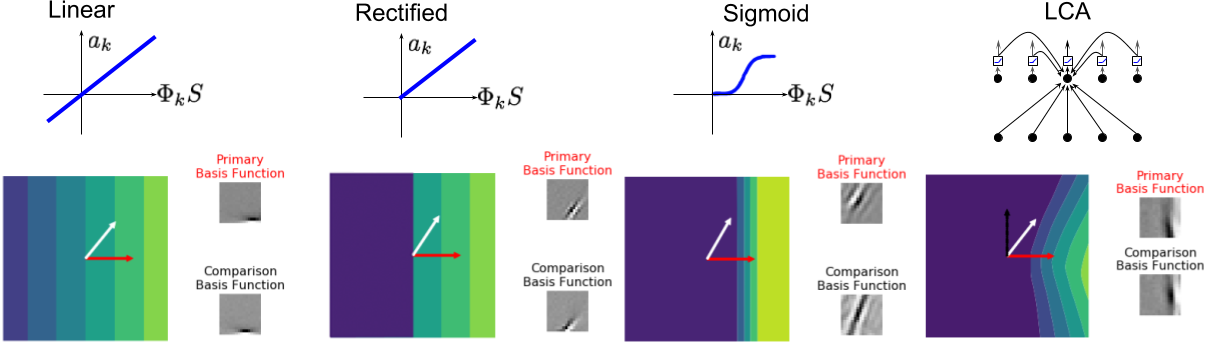
\includegraphics[width=0.5\textwidth]{figures/iso_contour_comparison.png}}
\end{center}
%\vskip -0.3in
\caption{Empirically measured iso-response contours. A fine sampling of points in the 2D plane are injected into the high dimensional image space and used as inputs to a target model neuron, $a_{k}$. The color value indicates a binned normalized response magnitude of the neuron. The red arrow is the weight vector for the neuron, $\phi_{k}$. The white arrow is an alternate neuron's weight vector.}
\end{figure}

%A histogram of 2nd order coefficients for polynomial fits to the lines in the middle plot. Negative coefficients indicate exo-origin curvature, which tells us that this neuron exhibits exo-origin curvature in all orthogonal directions tested.

\subsection{Population nonlinear neurons can be more robust to adversarial examples}
It is important to determine the shape of an individual neuron’s response contours for a large number of planes to better understand its high-dimensional geometry.  To do this, we used two different methods for choosing image planes. For both methods, we defined the horizontal axis as the weight vector (or basis function) for the target neuron. For the first method, we found a set of random vectors that are orthogonal to our target neuron’s weight vector and compute curvature in each plane. For the second method we start by finding another neuron’s weight vector that has a nonzero inner-product with our target neuron’s weight vector (and thus they are not orthogonal). Next, we used the Gram-Schmidt process to find a vector that is orthogonal to our target neuron, but coplanar with our second neuron. This method will increase the likelihood of competition between neurons, and thus increases the curvature. The result is shown in figure \ref{fig:figure} and indicates that the neuron’s high-dimensional iso-response geometry is cone shaped, with negative curvature in every direction.

\begin{figure}\label{fig:ch4_adv_grads}
%\vskip -0.05in
\begin{center}
\centerline{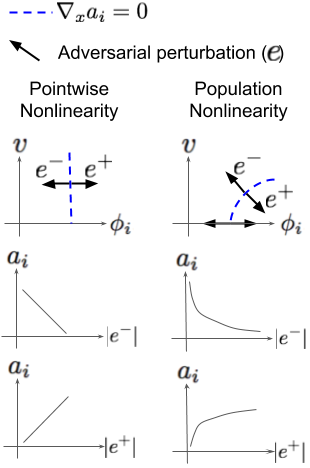
\includegraphics[width=0.5\columnwidth]{figures/adversarial_gradients_iso_contours.png}}
\end{center}
%\vskip -0.3in
\caption{Adversarial gradients (dark arrows) are always orthogonal to the iso-response contours (blue dashed line).$\Phi_{k}$ indicates a weight vector for the neuron $a_{k}$, and $v$ represents a random orthogonal direction.}
\end{figure}

Recall that the adversarial objective in equation \ref{eq:ch4_adv_metric} has an absolute value and is thus bi-directional. For a locally linear approximation of an untargeted attack, these two directions are equal. However, if we impose a rectifying constraint on our neuron outputs, then the two solutions are not equal for an individual neuron. For a sufficiently large $e$, the direction that lowers $a_{k}$ to below threshold will result in $f(s+e)=0$, i.e. $\max_{e^{-}}|f(s+e)-f(s)| = f(s)$. In other words, for rectified units, $\max_{e^{-}}|f(s+e)-f(s)|$ could be less than $\max_{e^{+}}|f(s+e)-f(s)|$. This would not be known to a simple gradient method for computing an non-targeted adversarial attack, such as that proposed in equation \ref{eq:ch4_adv_metric}. However, in practice actual adversarial attacks have an additional goal in mind: to produce an output that is reasonable for some \emph{other} data sample. Turning off all of the units in a layer is not a solution to this problem, so some set of adversarial perturbations must be in the $e^{+}$ direction. By definition, these perturbations will have greater contribution to the model's output than $e^{-}$ perturbations.

The Locally Competitive Algorithm (LCA) is a neural network with population nonlinearities that exhibits exo-origin bent iso-response contours. If the LCA is also rectified, then the $e^{-}$ direction will eventually turn off units. From figure \ref{fig:ch4_adv_grads} one can deduce that the only $e^{+}$ direction that will cause $a_{k}$ to grow without bound is along $\Phi_{k}$. What's more, \emph{all} directions that increase $a_{k}$ are towards, or along, $\Phi_{k}$. From this analysis we present three hypotheses:

\begin{itemize}
  \item Adversarial attacks on networks with exo-origin bent contours will be more aligned with the their weight vectors than attacks on networks with straight contours. If the weight vectors are data aligned then this will result in adversarial attacks that are data aligned.
  \item Rectified LCA should be resistant to unbounded adversarial attacks.
  \item Non-rectified LCA should be more susceptible to adversarial attacks than rectified LCA.
  \item More overcompleteness causes more bending of the iso-response contours \parencite{golden2016conjectures}, which will result in better adversarial defense.
\end{itemize}

In the following section we will outline several models used for our experiments as well as the experiments performed. Then we will present results that support the above hypotheses. Finally we will discuss the implications of these results and propose continued directions for research.

%\section{Comparison Models}\label{sec:ch4_comparison_models}
%We compared the LCA responses against a variational autoencoder \parencite{kingma2013auto}.
%The comparison models are:
%  * MLP (tensorflow tutorial)
%  * Sparse Autoencoder
%  * [Deep/Shallow] Variational Autoencoder
%  * LISTA

\section{Experiments on the MNIST dataset}\label{sec:ch4_mnist_experiments}
We suggest that the LCA requires stronger adversarial perturbation magnitudes to achieve the same change in the network output when compared to more standard feedforward autoencoders. Additionally, adversarial perturbations for the LCA are more aligned with the data than those for the alternative models tested. We have shown that both of these properties can be explained by an LCA neuron's exo-origin bent iso-response contours. We believe that this study synergizes with the works of \parencite{zhu2013visual} and \parencite{golden2016conjectures}, which together suggest that explaining-away process inherent in the sparse coding model produces a more selective and robust code of input data.

To begin testing our hypothesis, we followed the procedure outlined in \parencite{kos2018adversarial} to construct generative adversarial attacks. We consider the LCA as an autoencoder model, $\hat{s}=f(s)$, which encodes images into a latent space and then produces reconstructions from this encoding. We compare the LCA against the following models:

\begin{itemize}
  \item A sparse autoencoder (SAE, \parencite{ng2011sparse}) with a single overcomplete hidden layer that uses a pointwise sigmoid nonlinearity.
  \item A pointwise rectified (ReLU) \parencite{hahnloser2000digital, nair2010rectified} autoencoder with a single overcomplete hidden layer.
  \item A deep bottleneck pointwise rectified (ReLU) autoencoder.
  \item A deep variational autoencoder \parencite{kingma2013auto}.
\end{itemize}

  For the attack, an input image, $s$, was minimally perturbed before being passed through the autoencoder to produce a reconstruction of an entirely different target image, $s_{t}$. First, we found that the angle of the perturbed inputs, $s^{*}$, were closer to the target for LCA than for the SAE (figure \ref{fig:ch4_cosine_similarity}). We found that this performance difference was consistent through a sweep of attack parameters \ref{fig:ch4_kos_attack}. Next, we found that for attacks that did not include a clipping step to force the perturbation to be a certain size, the SAE perturbation grew without bound while the LCA perturbation settled to a fixed distance from the input (figure \ref{fig:figure}). Finally, to test whether this phenomena could result in improved adversarial robustness for classification networks, we compared a 2 layer neural network (MLP) with ReLU nonlinearities trained to identify the digit classes in the MNIST dataset against a single layer ReLU classifier (SLP) trained on the latent code produced by LCA. We found that the LCA+SLP model required a larger perturbation from the original input (as measured by mean squared error, MSE) for equal adversarial confidence than the MLP. Additionally, we found that the perturbations themselves were more semantically meaningful for the LCA+SLP than for the MLP (figure \ref{fig:ch4_latent_attac_mse}).

%In the following we will conduct several different adversarial attack experiments on a variety of models. The attacks are:
%  * Generative adversarial attack (kos)
%      - explanation
%  * Pixel classification attack
%      - explanation
%  * Latent classification attack
%      - explanation

\subsection{LCA Adversarial Attacks are Data Aligned}
In section \ref{neuron}, we showed that adversarial gradient directions for LCA neurons will point in data directions. To assess whether this result extends to the entire network, we measured the cosine similarity between an input image and a successful adversarial perturbation. Figure \ref{fig:ch4_cosine_similarity} demonstrates that adversarial perturbations for the LCA have a higher cosine similarity to the target image in a generative adversarial attack \parencite{kos2018adversarial} than the SAE. This indicates that the perturbations are more closely aligned to data directions, which should result in more semantically meaningful perturbations.

\begin{figure}\label{fig:ch4_cosine_similarity}
%\vskip -0.05in
\begin{center}
\centerline{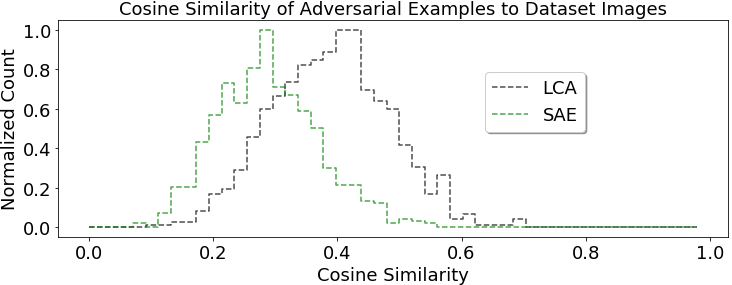
\includegraphics[width=\columnwidth]{figures/cosyne_similarity.png}}
\end{center}
%\vskip -0.3in
\caption{Adversarial attacks using gradients from the LCA have a larger cosine similarity to dataset images than attacks for the SAE. Following \parencite{kos2018adversarial}, we attacked each model using a target image that was an alternate image from the dataset. The histograms are computed over 800 image examples.}
\end{figure}

To understand how adversarial attacks transfer between these models, we produced adversarial images for each one and test how adversaries generated for one model affect another.

%TODO: The data-aligned perturbations can explain why adversarial images for LCA transfer to SAE and VAE but not the other way around \ref{fig:figure}.

\subsection{Pixel classification attack}
The standard attack method for classification networks is to perturb input pixels to result in misclassification. One proposed defense against this type of attack is to preprocess the image pixels with a denoising autoencoder that would produce reconstructions void of the adversarial pixel perturbations. However, it has been shown that if one backpropagates the adversarial loss through the autoencoder network, then it is still possible to adversarially attack the network. Here we show that the LCA model outperforms the VAE and SAE networks as a preprocessing \"firewall\" against the adversarial attacks.

\subsection{Generative adversarial attacks}
Recent results from \citet{kos2018adversarial} show that adversarial stimulus can be constructed for generative models. This is especially compelling because generative models are explicitly trained to preserve information about the input and produce a veridical reconstruction, whereas classification networks are typically trained to throw away large amounts of information and only preserve that which is relevant for the given task. We show that the LCA model is robust against generative adversarial attacks when compared to the SAE and VAE networks.

%
% * best solution is identity, but that is not an interesting solution
% * this attack prefers simpler models
% * which is why we include sae w/ tied weights
%

\begin{figure}[h]\label{fig:ch4_kos_attack}
%\vskip -0.05in
\begin{center}
\centerline{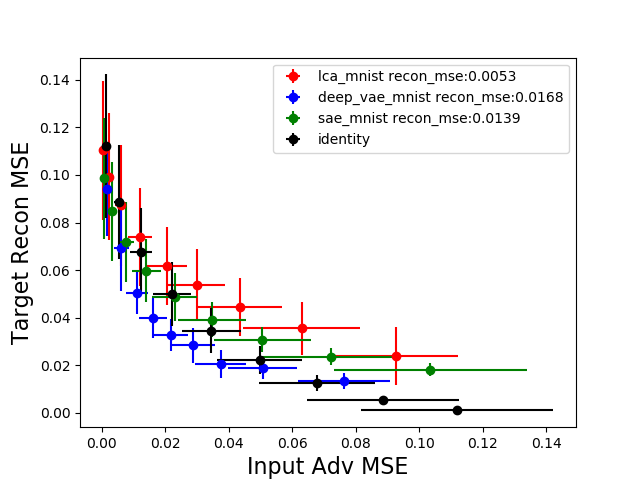
\includegraphics[width=\columnwidth]{figures/recon_mult_tradeoff.png}}
\end{center}
%\vskip -0.3in
\caption{TODO}
\end{figure}

\subsection{Latent classification attack}
The lateral connectivity in the LCA network is utilized via a recurrent computation. These dynamics facilitate a form of explaining away, where neurons that have a high degree of correspondence with the input stimulus suppress other neurons in the network. This results in the network ignoring input pixels that are not aligned with primary data directions. To better understand the role of the recurrent computation, we trained a network that acts as an unrolled version of LCA, where the lateral connectivity and feedforward weight matrices are learned. The LISTA model was demonstrated by Gregor et al. \citeyearpar{gregor2010learning} to show that a network with many fewer inference steps can produce codes that have a small Euclidean distance to the outputs of sparse coding. We trained three LISTA models with 5, 20, and 50 layers. All three models were trained to produce codes that had approximately the same $L_{2}$ distance from the codes produced by LCA. We show that the LISTA network does not perform as well as LCA at defending against adversarial attacks and that the deeper LISTA networks perform better.

\begin{figure}[h]\label{fig:ch4_latent_attac_mse}
\vskip -0.05in
  \begin{subfigure}
    \centering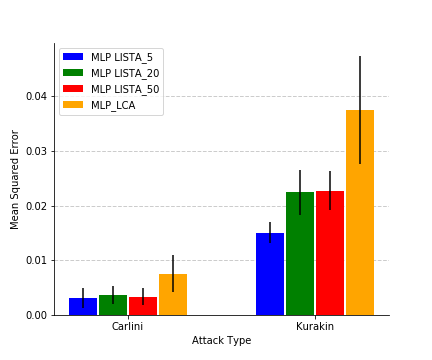
\includegraphics[width=\columnwidth]{figures/latent_clf_attack_mse.png}
  \end{subfigure}
  \begin{subfigure}
    \centering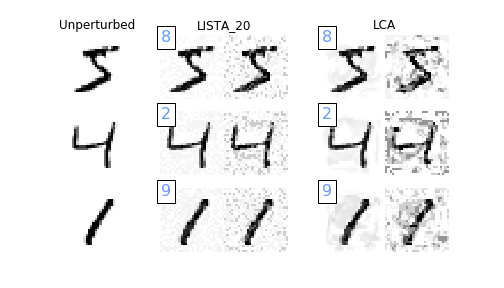
\includegraphics[width=\columnwidth]{figures/latent_clf_attack_ex.png}
  \end{subfigure}
\caption{LCA better protects against latent classification attacks. We generated adversarial examples from equal-sized MLPs trained from the latent codes of each model. MSEs were calculated between the original image and the perturbed image.   Error bars indicate standard deviation for 100 example inputs.}

\end{figure}

\subsection{Attacks with the CIFAR dataset}
The LCA objective is derived from a model of natural images, so we believe the network will exhibit stronger aversion to adversarial perturbations.
%%%% From paper

\section{Explaining increased orientation selectivity}
A longstanding hypothesis in visual neuroscience is that sensory neurons are adapted to natural image statistics to produce an efficient code. Independent Component Analysis (ICA) has been proposed as a normative model for simple cells in V1 based on its ability to reduce higher-order redundancy in natural images. When applied to natural images, the filters that emerge resemble the localized, oriented, and band-pass receptive fields of V1 neurons. However, quantitative analyses of the coding efficiency of ICA show that the neural code it produces fails to provide any appreciable gain in redundancy reduction beyond second-order methods such as PCA. This result appears to challenge the higher-order redundancy reduction account of V1 function. We explain these findings by distinguishing oriented filters from orientation \textit{selectivity} and show that ICA's linear encoding scheme fails to implement genuine orientation selectivity, which limits its capacity to learn an efficient code. We show that sparse coding, a related model with a nonlinear encoding scheme that produces orientation selective neurons, is able to achieve a more efficient code than both ICA and PCA when evaluated in the rate-distortion framework, thus providing renewed support for the efficient coding account of V1 receptive field properties.

A long-standing hypothesis in sensory neuroscience proposes that a primary function of early sensory processing is to form an efficient, redundancy-reduced code of the input that maximizes the brain's limited computational and biological resources while making explicit the statistical structure of the input \parencite{barlow2001redundancy}. This hypothesis predicts that the response properties of sensory neurons should be adapted to the statistical structure of their input.

In support of this hypothesis, a number of the response properties of visual neurons have been reproduced by optimizing redundancy-reducing linear transformations on natural images \parencite{atick1990towards}. For example, a symmetric decorrelation transformation of natural images yields center-surround receptive fields \parencite{atick1990towards}, and Principal Component Analysis (PCA) applied to color images yields the luminance, red-green, and blue-yellow channel observed in the opponent color coding of retinal ganglion cells \parencite{ruderman1998statistics, buchsbaum1983trichromacy}. When higher-order correlations are additionally reduced, localized and oriented band-pass filters that resemble the orientation-selective receptive fields in V1 emerge \parencite{bell1997independent, olshausen1999probabilistic}. It has thus been proposed that the oriented filters in V1 function to remove higher-order correlations.

Orientation selectivity is a striking feature of the response properties of simple cells in V1. Since the discovery of orientation selectivity in Hubel and Wiesel's Nobel Prize-winning work, the mechanism for the computation has remained unclear. A common point of confusion in the field has been the assumption that a neuron with an locally oriented receptive field will exhibit orientation selectivity. Here, we will argue that orientation selectivity requires a non-linear encoding process in addition to an oriented receptive field.

Independent Component Analysis (ICA) is one of the most widely used image coding algorithms and has been proposed as a model for simple cells in V1 \parencite{bell1997independent}. The ICA algorithm explicitly optimizes for higher-order redundancy reduction, aiming to to reconstruct the input image as a linear superposition of a set of basis functions while minimizing the mutual information between those bases.

\citeit{eichhorn2009natural} compare the  coding efficiency of ICA and PCA to obtain the surprising result that ICA performs no better than PCA on a rate-distortion trade-off metric. ICA is trained with the objective of minimizing the joint entropy of the activations and learns oriented filters that suggest it has succeeded in modeling higher-order pixel correlations, while PCA is a second-order method that does not learn oriented filters. \citeit{eichhorn2009natural} argue that if ICA had succeeded at capturing higher-order statistics, it should show an advantage in the rate-distortion trade-off.

We present an alternate explanation of these findings by distinguishing \textit{orientation selectivity} from \textit{oriented filters}. Neurons achieve orientation selectivity via a fundamentally nonlinear process, as exhibited by nonclassical receptive field (nCRF) effects such as cross-orientation suppression \parencite{golden2016conjectures, zhu2013visual}. We argue that although the ICA optimization algorithm is able to learn oriented filters, ICA's linear encoding process limits its capacity to perform genuine orientation selectivity, which in turn limits its capacity to produce an efficient code. \citeit{zhu2013visual} demonstrate that sparse coding is able to provide a parsimonious explanation of both classical and nonclassical receptive field properties using a neural network implementing sparse coding \parencite{zhu2013visual}. Here, we replicate the rate-distortion analyses from \citeit{eichhorn2009natural} using the sparse coding network described by \citeit{zhu2013visual} to show that a nonlinear encoding process produces more efficient codes to linear encoders. To assess the degree of orientation selectivity for ICA neurons, we replicate the cross-orientation suppression experiment performed by \citeit{zhu2013visual} with both sparse coding and ICA networks.


%% TODO:
\subsection{Rate-distortion analyses}
The Shannon standard for evaluating the efficiency of lossy continuous codes is the rate-distortion framework \parencite{cover2012elements}. \citeit{eichhorn2009natural} compare the  coding efficiency of ICA and PCA and find that PCA performs \textit{better} than ICA in terms of the rate-distortion trade-off. This result is surprising in that ICA is explicitly trained with the goal of minimizing the joint entropy of the activations and learns oriented filters that would suggest that it achieved the goal of modeling higher-order correlations, while PCA is a second-order method that does not learn oriented filters.

We resolve this apparent paradox by distinguishing \textit{orientation selectivity} and \textit{oriented filters}. Neurons achieve orientation selectivity via a fundamentally non-linear process, as exhibited by non-classical receptive field (nCRF) effects such as contrast invariant tuning and cross-orientation suppression \parencite{ferster2000natural,  zhu2013visual}. We argue that although the ICA optimization algorithm is able to learn oriented filters, ICA's linear encoding process limits its capacity to perform genuine orientation selectivity, which in turn limits its capacity to produce an efficient code. Sparse coding is unique in its ability to provide a parsimonious explanation of both classical and non-classical receptive field properties \parencite{zhu2013visual, golden2016conjectures}. Although nCRF effects are typically modeled individually, \citeit{zhu2013visual} show that a wide variety of these effects are emergent properties of a neural network implementing sparse coding. * something about LCA * These findings suggests the primacy of efficient coding in V1. This explanation only holds, however, if sparse coding can be quantitatively shown to achieve a gain in coding efficiency beyond second-order methods. Here, we replicate the rate-distortion analyses from \citeit{eichhorn2009natural} and show that the LCA's non-linear encoding process enables codes that are lower entropy than those learned by ICA or PCA while being more perceptually robust to increasingly coarse quantization.


\subsection{Methods and Results}
We train sparse coding \parencite{rozell2008sparse}, ICA \parencite{bell1997independent}, and PCA on 1 million 16 x 16 pixel grayscale image patches extracted from images in the van Hateren dataset of natural scenes, which have been transformed to log intensity and standardized to zero mean and unit variance \parencite{vanHateren1998independent}. Using the learned filter matrices, we compute model activations for a test set of 100,000 patches and uniformly quantize these activations with varying degrees of granularity. For each level of granularity, we compute a reconstruction of the test input using the quantized activations and compute the mean squared error. Figure \ref{fig:ch4_rd_curve} plots the rate (mean marginal discrete entropy of the activations) against the distortion (mean squared error).

%\begin{figure}[ht]\label{fig:ch4_rd_curve}
%\vskip 0.1in
% \centering \includegraphics[width=\linewidth]{figures/rd_curves.png}
% \caption{Discrete entropy vs. reconstruction error for sparse coding, PCA, and ICA.}
%\vskip -0.2in
%\end{figure}

Results for sparse coding models trained with different values of $\lambda$ are shown, where a larger $\lambda$ indicates higher sparsity. We replicate the findings from \citeit{eichhorn2009natural} that (orthogonal) PCA  performs slightly better than ICA in the rate-distortion trade-off. Sparse coding shows an advantage over both ICA and PCA. Additionally, we find that representations that are more sparse are capable of achieving increasingly lower rates. Figure \ref{fig:ch4_rd_recons} shows an example reconstruction in the highly lossy (low entropy) regime. For a mean marginal entropy of $H\approx 0.4$, sparse coding shows an advantage in perceptual quality, as well as a quantitative advantage in terms of mean squared error.

%\begin{figure}[ht]\label{fig:ch4_rd_recons}
%\vskip 0.1in
% \centering
% \includegraphics[width=\linewidth]{figures/baboon_4_square.png}
% \caption{Lossy reconstructions for quantized activations with mean marginal entropy $H\approx 0.4$}
%\vskip -0.2in
%\end{figure}


\subsection{Discussion}
Our results suggest the importance of nonlinear encoding for learning efficient codes of natural images and demonstrate that orientation \textit{selective} neurons are capable of reducing higher-order redundancy. We show that although the ICA algorithm is able to learn oriented filters, ICA's linear encoding process limits its capacity to perform genuine orientation selectivity, which in turn limits its capacity to produce an efficient code. 

Although sparse coding produces a more efficient representation of natural image and neurons that have a higher degree of orientation selectivity than ICA, the model is nonetheless fundamentally limited in its capacity to fully characterize the statistics of natural scenes because it assumes a linear generative model and the light that forms images is combined in a non-linear fashion, such as by occlusion. In future work we plan to extend our analysis to hierarchical models of natural scenes that may achieve greater gains in coding efficiency.

The efficient coding hypothesis was initially posed in terms of redundancy reduction \parencite{barlow1961possible}, under the hypothesis that the brain may seek an efficient code of the input in order to minimize the number of neurons required to represent the signal. Anatomical evidence tells us, however, that the V1 expands the image representation coming from LGN by having many more outputs than inputs \parencite{olshausen2003principles} Thus, redundancies are actually \textit{created} in the perceptual process. The goal of cortical processing, then, cannot be said to be redundancy reduction and simple compression.

As an alternative, several researchers have argued that the goal of perception cannot be discussed in isolation from action; an organism forms perceptual representations for the purpose of directing its behavior towards the achievement of desirable outcomes and away from undesirable ones \parencite{barlow2001redundancy, simoncelli2001natural}. From this perspective, the brain aims to extract the statistical structure of the input in order to form a``meaningful'' representation that recovers the environmental causes of the sensory data, which it can use to guide action. Along these lines, the efficient coding hypothesis has been revised to emphasize redundancy \textit{representation} rather than reduction \parencite{barlow2001redundancy}. Redundancies in the input signal indicate structure in the environment. An encoding that makes these redundancies explicit encodes the causal and statistical structure of the environment, which the organism can exploit to plan and direct behavior.

Sparse coding performs redundancy representation rather than redundancy reduction. A sparse code is a highly redundant code It has been demonstrated that a typical redundancy reducing code--which would form a distributed representation of the input with a high activity ratio--would actually lead to large errors in estimates of the frequency of a particular input, since many neurons are active in response to both the input of interest as well as other stimuli \parencite{gardnermedwin2001limits}. A sparse code, in which the elements of the learned dictionary occur independently in the environment, is a factorial code; the probability of any composite image is simply the product of the probabilities of the components. Any deviations from this rule signal a previously unknown statistical dependency to be learned.

 An efficient code exploits the redundancies in the input signal. The objective of early sensory processing was initially described as redundancy reduction. The redundancy reduction hypothesis was partially motivated by the observation that a significant information bottleneck exists in the first stage of visual processing; most mammals have vastly more photoreceptors than fibers in the optic nerve, which suggests that significant compression must occur in the first stage of processing. However, at moderate to high luminance levels, only a small subset of the photoreceptors are operating within their dynamic ranges; thus the reduction in capacity may be smaller than initially implied. Further, beyond the optic nerve, the number of neurons involved in subsequent layers of processing generally increases, which means that redundancies are actually created in the perceptual process. The goal of early vision, then, cannot be said to be redundancy reduction. From a functional standpoint, several researchers have also argued that the goal of perception is not simple compression; an organism forms perceptual representations in order to direct its behavior towards the achievement of desirable outcomes and away from undesirable ones \parencite{barlow2001redundancy, simoncelli2001natural}. From this standpoint, one can argue that brain aims to extract the statistical structure of the input in order to form a \textit{meaningful} representation that recovers the environmental causes of the sensory data, which it can use to guide action.
 
 Along these lines, the efficient coding hypothesis has been revised more recently to emphasize redundancy representation rather than reduction \parencite{barlow2001redundancy}. Redundancies in the input signal indicate structure in the environment. An encoding that makes these redundancies explicit encodes the causal and statistical structure of the environment, which the organism can exploit to plan and direct behavior. Barlow further argues that to facilitate the identification of the statistics of the environment, neural responses should form a sparse code of the input. He notes that a typical redundancy-reducing code would be a distributed representation of the input with a high activity ratio–that is, a large percentage of active neurons, each of which is frequently active across different inputs. Such a code will lead to large errors in estimates of the frequency of a particular input, since many neurons are active in response to both the input of interest as well as other stimuli. A sparse code, in which the elements of the learned dictionary occur independently in the environment, would form a factorial code, in which the probability of any composite image is simply the product of the probabilities of the components. Any deviations from this rule would signal a previously unknown statistical dependency to be learned.
 
%%%% From paper
Although the softmax nonlinearity used in most classification models is a population nonlinearity, we hypothesize that an adversarial image perturbation can produce adversarial inputs to the softmax, negating it's ability to protect the network against the attack.

Additional control models need to be explored, including alternative population nonlinearities such as those present in Boltzmann machines \parencite{salakhutdinov2009deep}, divisive normalization \parencite{balle2016end}, and local response normalization \parencite{krizhevsky2012imagenet}. Each of these nonlinearities has had significance in the deep learning and neuroscience communities. The iso-response analysis provides a methodology for contrasting them and will give us valuable insight into how each of them may respond to adversarial attacks. We also wish to scale up the models to include larger datasets of more naturalistic images. 

Hierarchical extensions to the sparse coding model \parencite{chen2018sparse} have been shown by our group to perform a better job of mapping input data onto a smooth manifold. We hypothesize that this will further increase the semantic relevance and model robustness for adversarial perturbations. We intend to include the model defined in \parencite{chen2018sparse} in our future analysis to explore how the adversarial and iso-response properties change as we increase the network depth.

This methodology has a high potential for impact in the deep learning community. We advocate for biologically motivated computations that go beyond the simple pointwise nonlinear model. We have shown that these types of networks learn a more robust representation of data without tedious and biased human labeling. We also provide strong theoretical support for our hypotheses and an analysis method that allows us to fully characterize how the more complicated neurons will respond to input perturbations.
%%%%

\section{Explaining extra-classical receptive field effects}
Golden, explaining others.


\section{Applications to physiological neuroscience}
Use this method to probe neuron contours.\label{ch:semi-supervised}
\chapter{Iso-Response Contours Provide a Geometric Interpretation of Neurons}

%%%% From paper
\section{Introduction}\label{intro}
%* Theories for how/why attacks happen
%- cascading linearity (goodfellow et al. 2015)
%- excessive invariance
%- subspace view
%- classication boundary curvature view
%- ford et all adv examples & noise
%    * adv examples are the nearest test error
%    * although our model doesn't have better test error, we argue that the nearest point is more data-aligned.
%    * We should also test against distribution shift (fig 7, right from their paper)
%    
%* Defense methods
%- supplementing the dataset with adversarial examples
%- augmenting loss function with adv loss (madry)
%- preprocessing / denoising images (although this is difficult to do without heavily reducing model performance)
%
%* Models that have relevance to ours:
%- sun et al (sparse coding, although they are also obfuscating gradients)
%- marzi et al (sparsity, although they are also obfuscating gradients)
%- DARCCC (population nonlienarity?)
%* Find more papers that look at adversarial images compared to the image manifold \parencite{sun2018adversarial}.

Adversarial examples are a demonstration of an ANN’s inability to cope with a distributional shift from its training data \parencite{ford2019adversarial}. They represent a worst-case demonstration of this weakness, which is a general problem that all classification ANNs are susceptible to \parencite{hendrycks2018benchmarking}. We postulate that designing machine learning algorithms that are both accurate and robust to adversarial attacks requires a radical reformulation in how such algorithms are currently constructed. In particular, we propose to abandon a strict reliance on reducing classification loss (i.e. an exclusive focus on classification accuracy) and instead allow our models to undergo a period of unsupervised learning that mimics the cognitive development of biological nervous systems. Biological systems are robust to adversarial examples that affect deep networks. However, in time-limited regimes that result in predominantly feed-forward brain computation adversarial attacks have been shown to influence human decision making \parencite{elsayed2018adversarial}, suggesting that slower recurrent feedback loops aid in adversarial robustness. Furthermore, congruent with current theories for probabilistic inference in the brain \parencite{lee2003hierarchical}, we augment the standard ANN architecture with lateral connectivity and recurrence. We propose that, together, these innovations will improve the network’s specificity to signals that lie along the data manifold. We use adversarial attacks as a mechanism for understanding both traditional pointwise nonlinear ANNs and a population nonlinear alternative.

Adversarial attacks represent a recently discovered flaw in typical deep neural networks, where small targeted perturbations in the input space can cause large undesired changes in the output space. Although the discovery of adversarial examples in deep networks is relatively new, a fervor of research has produced a large body of literature on the subject and an understanding of these attacks has begun to emerge. In the pioneering work of Szegedy et al. \citeyearpar{szegedy2013intriguing}, they introduce the idea of ``adversarial attacks'' for deep networks and propose that a non-smooth decision boundary in classification networks produces adversarial ``pockets'' interspersed among dataset examples. They also suggest that adversarial images represent a counter-example to the hypothesis that deep networks are able to achieve local generalization to input space regions in the vicinity of training examples. Although this latter hypothesis has continued to hold, the presence of universal and transferable adversarial directions \parencite{moosavi2017universal} suggests that there are not adversarial pockets in the input manifold. The follow up work of Goodfellow et al. \citeyearpar{goodfellow2014explaining} make several proposals, some of which have been refuted \parencite{jetley2018friends}. However, we would like to emphasize two important arguments from their work: 1) they present evidence suggesting that the direction of perturbation is more important than the specific point in space (further refuting the ``pockets'' theory), and 2) the adversarial perturbations are highly aligned with the weight vectors of a model. The last of those observations has been explored in much more detail by Jetley et al. \citeyearpar{jetley2018friends}, who suggest that deep networks produce classification boundaries based on a small number of features that correspond to high curvature directions in the input space and that these high curvature directions are also the most effective adversarial directions. The works of Gilmer et al. \citeyearpar{gilmer2018adversarial} and Ford et al. \citeyearpar{ford2019adversarial} further expand on this idea by suggesting that adversarial attacks confined to the $l_{\infty}$ box represent the worst-case example of the model's inability to account for distributional shift generally. However, the works of Kos et al. \citeyearpar{ford2019adversarial} and Goodfellow et al. \citeyearpar{goodfellow2014explaining} demonstrate the ability to produce adversarial examples for pointwise-nonlinear generative models that have applications in image denoising, suggesting a more nuanced explanation of adversarial susceptibility. Recent work has also shown that nearly all proposed adversarial defense mechanisms fail in the face of more careful attacks \parencite{carlini2017towards, athalye2018obfuscated}.  For example, the recent defense method proposed by \parencite{sun2018adversarial} claims to produce an adversarially robust preprocessing step, although they use basis pursuit in their methods, which possibly achieves robustness through gradient obfuscation \parencite{athalye2018obfuscated}. However, their intuition that images should be forced onto the image manifold as a preprocessing step has great relevance to the work herein. It will always be possible to produce an image perturbation that results in a change in class label, or an alternate reconstruction. The academic fascination in the subject comes from observations of how small that perturbation needs to be and the (lack of) semantic content of the perturbation. Following the intuition provided in \parencite{ford2019adversarial}, successful defenses appear to require accomplishing one of two goals: 1) robustly denoising inputs to prevent distributional shift or 2) training deep networks to be more robust to worst-case distributional shift.

Inferring causes from natural signals is a challenging problem faced by biological vision systems. For artificial vision, the neural network community has largely tackled this problem using feedforward discriminative models. An alternative approach is to use generative models, in which the network must attempt to explain data in terms of an internal model of the world. In BNNs we see a preponderance of evidence that individual neurons are highly non-linear, recurrent, and laterally connected. The Locally Competitive Algorithm (LCA) \parencite{rozell2008sparse} is a generative sparse coding model that represents an example of how lateral inhibition can be derived from a well-defined computational objective. This network has been shown previously to exhibit a variety of non-linear receptive field effects \parencite{zhu2013visual}. Many of these effects can be explained using the model neuron’s iso-response contours - a common experimental method in neuroscience for determining stimulus combinations that result in equal activation from recorded neurons \parencite{golden2016conjectures}. In the brain, the atomic unit of computation is generally considered to be the neuron, but most deep learning research has eschewed the individual neuron, possibly obfuscating the connections between BNNs and ANNs. We propose to adopt the single-neuron iso-response analysis to better understand adversarial attacks on ANNs while varying degrees of biological realism.

To better understand how adversarial attacks differ for BNNs and ANNs, we compared feed-forward, pointwise nonlinear discriminative and generative network architectures against more biologically informed population nonlinear generative network architectures. Pointwise nonlinearities are the more traditional form of nonlinearities, as seen in nearly all deep neural network architectures. They are defined as nonlinearities that are a function of only a single neuron in a layer and include rectification, sigmoid, and hyperbolic tangent. Population nonlinearities represent the alternative class, where the nonlinearity output is a function of multiple neurons in a set. These include softmax, divisive normalization \parencite{carandini2012normalization, balle2016end} and the network nonlinearity present in sparse coding \parencite{rozell2008sparse, olshausen1997sparse}. In principle, generative models should not be as susceptible to adversarial attacks as discriminative models because they are trying to fit their internal model to the data as a ``sanity check'', which should not succeed for adversarial perturbations. One method by which generative models can perform such a sanity check is via recurrent maximum a-posteriori (MAP) inference. The LCA network uses population nonlinear interactions via lateral connectivity among neurons to facilitate this process, resulting in an ``explaining away'' effect commonly referenced in Bayesian inference literature \parencite{olshausen2014perception, citation}.

Here, drawing from the architecture and function of brains, we propose that a network with lateral inhibitory connectivity in its hidden layer forces adversarial perturbation vectors to have angles that are more in line with data dimensions, producing more semantically meaningful perturbations. We develop an analytic argument to support this claim for untargeted adversarial attacks. Furthermore, we demonstrate by experiment that our method successfully improves robustness to adversarial attacks and more broadly distributional shift for a classifier trained on our model's outputs. The contribution of our work is a novel perspective for understanding adversarial attacks and population nonlinear networks. We also demonstrate that simple generative models can be used to improve a typical network’s defenses against adversarial attacks.

\section{Neuron response geometry explains adversarial robustness}\label{neuron}
We propose to perform single neuron and population level analysis by extending the iso-response contour theory to be used as a lens to understand untargeted adversarial perturbations for individual neurons. Additionally, we have scaled up the iso-response analysis to models trained on images of handwritten digits (MNIST, \parencite{citation}) and natural scenes (CIFAR, \parencite{citation}). We show that the response geometry of LCA neurons predicts data-aligned perturbations when attacking the entire network, resulting in semantically meaningful adversarial attacks. We provide a theoretical argument to support this intuition by exploring the iso-response contours and orthogonal adversarial directions for individual neurons and give empirical evidence to further bolster the claims. 

Biological neurons are highly interconnected, both across and within layers. This interconnection gives rise to strong population nonlinear effects. However, nearly all work in neuron modeling uses pointwise nonlinearities due to the ease in interpretation and implementation. Work from \citeyearpar{golden2016conjectures} suggests a novel single-neuron analysis technique that allows us to increase the complexity of our neuron models without decreasing our understanding by looking at the neuron’s response geometry. We extend this technique to larger scale models that allows us to predict important properties about the model’s susceptibility to adversarial attacks. We then analyze the attacks themselves to demonstrate how the single-neuron analysis extends to networks. We conduct our preliminary experimentation on two types of networks: those with pointwise nonlinearities and those with population nonlinearities (Figure \ref{fig:pointpopnets}). Although there are many types of networks that fit into these two categories, we reserve comparative analysis among them to future work and focus this study on two specific instances: Feedforward Autoencoders (AEs) and the Locally Competitive Algorithm (LCA). We focus on the LCA as the population nonlinear network because it has been shown to exhibit many linear and nonlinear response properties that are well matched to what is observed in the brain \parencite{zhu2013visual, olshausen1997sparse}. The LCA was first proposed by Rozell et al. \citeyearpar{rozell2008sparse} to perform sparse coding. It is a generative network that uses MAP estimates of data likelihood to build an internal model. It can also be thought of as an auto-encoder with a single recurrent hidden layer. Details on these models can be found in section \ref{sec:models}.

\subsection{Adversarial examples are orthogonal to iso-response contours}
To better understand the difference between population and pointwise nonlinearities, we visualize the input-output maps of model neurons in the form of iso-response contours (Figure \ref{fig:iso_contours}, see caption for more details). Golden et al. \citeyearpar{golden2016conjectures} used iso-response contours to explain several non-linear properties as well as variance/invariance properties for simple and complex cells. To construct the visualization, we consider a two-dimensional slice, or projection, in the high dimensional input space. We use each point (i.e. image) in the slice as input to the neuron model and bin the points according to the neuron's output amplitude (Figure \ref{fig:iso_contours}). The iso-response contours of linear neurons are straight: any input perturbation that is orthogonal to the weight vector will result in equal activation. For pointwise nonlinearities, this remains true: because the nonlinearity is performed after a linear projection, the output must also produce straight iso-response contours. By contrast, for a population nonlinearity the gradient of the activation function with respect to a small perturbation in the input is a function of all other neurons in the layer. Thus, for a perturbation that is orthogonal to a target neuron, it is highly likely that an alternative neuron will have a non-orthogonal weight vector, which will result in a net change in all neuron outputs. Therefore, iso-response contours for population nonlinear neurons can be bent.

Adversarial examples are closely tied to neuron iso-response contours. While an iso-response contour represents a perturbation direction in stimulus space that produces no change in the output, an adversarial example is a perturbation direction that produces a maximal change in the output. Below, we present analytic arguments that these two response directions are orthogonal for individual neurons.

If we extend the work of Marzi et al. \citeyearpar{marzi2018sparsity} to include nonlinear functions, then we can define adversaries as seeking to maximize the following measure, $\Delta$, with respect to a perturbation, $e$:

\begin{align}\label{eq:adv_metric}
\begin{split}
    \max_{e} \Delta (s, s+e) = \max_{e} |f(s+e) - f(s)| \\
    s.t. \|e\|_{\infty} < \varepsilon,
\end{split}
\end{align}
where $f()$ can include a non-linear activation function, $s$ and $e$ are equal sized column vectors representing the data and perturbation, respectively, and $\varepsilon$ is some small scalar value. To solve this equation, one must find a perturbation that results in a model output that is maximally different from the output with respect to the original input. For our analysis, $e$ indicates a targeted perturbation of fixed magnitude that is subject to $|e|_{\infty}<\varepsilon$. By definition, for any vectors $u$ and $v$, $\langle u,v\rangle = |u| \cdot |v| \cdot cos(\Theta_{u,v})$. Going forward, we will reference the inner angle between two vectors as $\Theta_{u,v}$ for some vectors $u$ , $v$. If we assume that the perturbation magnitudes are fixed and equal, i.e.$|e_{adv}| = |e_{iso}| = k < \varepsilon$, then we can optimize over the angle between the perturbation vector and the input signal $\Theta{e,s}$. We can now include perturbation directions that result in a minimal change in the neuron's output:

\begin{center}
    \begin{tabular}{ |c | c| } \hline
     \textbf{Adversarial} & \textbf{Iso-Response} \\ \hline
     $\max_{\Theta_{e,s}}|f(s+e) - f(s)|$ & $\min_{\Theta_{e,s}} | f(s+e) - f(s) |$ \\ \hline
    \end{tabular}
\end{center}

These so called ``iso-response'' directions create contours in the neuron's response field. We can use the Fr\'{e}chet derivative \parencite{citation} to better understand how the neural response geometry relates to adversarial images:

\begin{align}\label{eq:frechet}
\begin{split}
    f(s+\varepsilon) &= f(s) + \langle\nabla_{s}f(s), \varepsilon\rangle + o(\varepsilon)\\
    &\therefore \\
    f(s+\varepsilon) - f(s) &= \langle\nabla_{s}f(s), \varepsilon\rangle+ o(\varepsilon),
\end{split}
\end{align}

where $\langle , \rangle$ indicates a dot product and $o(\varepsilon)$ is a tight bound that means ''terms that are, in the limit $\varepsilon \rightarrow 0$, dominated by $\varepsilon$\". Combining this with the bottom equality in equation \ref{eq:frechet} gives us:

\begin{align}\label{eq:angle_metric}
\begin{split}
    &\textbf{Adversarial:} \max_{\Theta_{e,s}} |f^{\prime}(s)^\top e + o(\|e\|)|,\\
    &\textbf{Iso-Response:} \min_{\Theta_{e,s}} |f^{\prime}(s)^\top e + o(\|e\|)|,
\end{split}
\end{align}

where $f^{\prime}(s) = \nabla_{s}f(s)$ is the output gradient of the target neuron. For small $\|e\|$, the linear terms in equation \ref{eq:angle_metric} dominate and these equations are solved when $e \parallel f^{\prime}(s)$ for the adversarial perturbation and $e \perp f^{\prime}(s)$ for the iso-response perturbation. This tells us that the optimal adversarial directions will always be perpendicular to the iso-response directions for an untargeted adversarial attack. 

\subsection{Iso-response contours}
Although we cannot analytically estimate the shape of the iso-response contours for population nonlinear neurons, we know that the adversarial directions will be perpendicular to them. Therefore, we can estimate adversarial perturbation directions by measuring the iso-response contours empirically. Figure \ref{fig:adv_grads} shows schematic drawings of the contours measured for population- and pointwise-nonlinear neurons along with the expected adversarial directions.

The response function of a model neuron for a perturbation, $e$, added to an input signal, $s$, can give us insight to that neuron's iso- and adversarial-response properties. First, we will describe this for a linear neuron, $a_{k}=f_{k}(s)=\phi_{k}^\top s$:

\begin{align}\label{eq:linear_neuron}
\begin{split}
    a_{k}(s+e) &= f_{k}(s+e) = \phi_{k}^\top (s + e) \\
    &= \phi_{k}^\top s +\phi_{k}^\top e,
\end{split}
\end{align}

where $\phi_{k}$ is a column weight vector. Next we match equation \ref{eq:linear_neuron} to the top part of equation \ref{eq:frechet}:

\begin{equation}
    f(s) + \langle\nabla_{s}f(s), e\rangle + o(\|e\|) = \phi_{k}^\top s + \phi_{k}^\top e.
\end{equation}

This tells us that the first term on the right hand side is $f(s)$ and the second term is $\langle\nabla_{s}f(s)^\top, e\rangle$, which means the third term is $o(||e||)=0$ (this is expected because it is a linear function). Therefore,  $\nabla_{s}f(s) = \phi_{k}$ and for any $e \perp \phi_{k}$, $f_{k}(s+e) = f_{k}(s)$. To summarize, for linear neurons:

\begin{align}\label{eq:parallel_adv_proof}
\begin{split}
    f(s) &= \phi_{k}^\top s \\
    f(s+e) &= \phi_{k}^\top s + \phi_{k}^\top e \\
    &\forall ||e||_{\infty} < \varepsilon \\
    &\therefore \\
    \max_{e} | f(s+e) - f(s) | &= \max_{e} | \phi_{k}^\top e | \\
    & \forall ||e||_{\infty} < \varepsilon
\end{split}
\end{align}

For a fixed amplitude perturbation, the maximum adversarial direction is when the inner angle $\Theta_{\phi_{k},e} = 0$. Additionally, perturbations that are orthogonal to $\phi_{k}$ are iso-response directions because they do not result in a change in $a_{k}$, which is illustrated in the top left plot of Figure \ref{fig:iso_contours}.

We can again use equation \ref{eq:frechet} to gain insight about the iso-response directions and adversarial directions for pointwise nonlinear functions, such that $a_{k}(s) = f_{k}(s) = g_{k}(\phi_{k}^\top s)$:

\begin{align}\label{eq:pw_nonlin}
\begin{split}
  a_{k}(s+e) &= g_{k}(\phi_{k}^\top(s+e)) \\
  &=g_{k}(\phi_{k}^\top s + \phi_{k}^\top e) \\
\end{split}
\end{align}

where $g_{k}(\cdot)$ is a pointwise non-linear activation function for neuron $k$. If we perform a change of variables such that $a = \phi_{k}^\top s$ and $b = \phi_{k}^\top e$, then we can fit equation \ref{eq:pw_nonlin} to match equation \ref{eq:frechet}:

\begin{align}\label{eq:pw_nonlin_frechet}
\begin{split}
    g_{k}(a + b) &= g_{k}(a) + \nabla_{s}g_{k}(a) \cdot b + o(b) \\
    &=g_{k}(\phi_{k}^\top s) + \nabla_{s}g_{k}(\phi_{k}^\top s) \cdot \phi_{k}^\top e + o(\phi_{k}^\top e)\\
    &=g_{k}(\phi_{k}^\top s) + \langle\nabla_{s}g_{k}(\phi_{k}^\top s) \cdot \phi_{k}^\top, e\rangle + o(\|e\|),
\end{split}
\end{align}

where $\cdot$ indicates pointwise vector multiplication. Now we match equation \ref{eq:pw_nonlin_frechet} to the bottom part of equation \ref{eq:frechet} to show 

\begin{equation}
\begin{split}
    |a_{k}(s+e) - a_{k}(s)| = |\nabla_{s}g_{k}(\phi_{k}^\top s) \cdot \phi_{k}^\top e + o(\|e\|)|.
\end{split}
\end{equation}

Again, the function is maximized when $\Theta_{\phi_{k}, e}=0$ and minimized when $\Theta_{\phi_{k}, e}=\tfrac{\pi}{2}$, which tells us that a pointwise nonlinearity can only change the spacing between the contours, it cannot bend the contours in any way.

Finally, we extend this analysis to population nonlinear networks. For population nonlinear networks, the output is now a function of the the other neurons in the layer as well as the input. Thus, $\Phi$ represents the entire weight matrix, with rows set to $\phi_{k}^\top$. We want to know how a small perturbation in the input changes \emph{all} of the outputs. We answer this by defining the activation gradient as:

\begin{align}\label{eq:pop_nonlinear}
\begin{split}
   a_{k}(s+e) &= p_{k}^\top g(\Phi(s+e)) \\
   &= p_{k}^\top g(\Phi s + \Phi e) \\
   &= p_{k}^\top g(\Phi s) + (\nabla_{s}g(\Phi s)^\top p_{k})^\top \Phi e + o(\|\Phi e\|) \\
   &= p_{k}^\top g(\Phi s) + (\Phi^\top \nabla_{s}g(\Phi s)^\top p_{k})^\top e + o(\|e\|),
\end{split}
\end{align}

where $p_{k}^\top$ is a one-hot vector selecting output $k$, $g(\cdot)$ is a function of all of the weight vectors and the input, and $\nabla_{s}g(\Phi s)$ is a Jacobian. We can no longer simply describe the contours of these neurons because the gradient of the non-linearity is now a function of (an arbitrary linear transformation of) $s$. For individual neurons, the contours can be straight or bent, and if bent they can bend towards the origin (endo-origin) or away from it (exo-orogin).

\begin{figure}[h]
%\vskip -0.05in
\begin{center}
\centerline{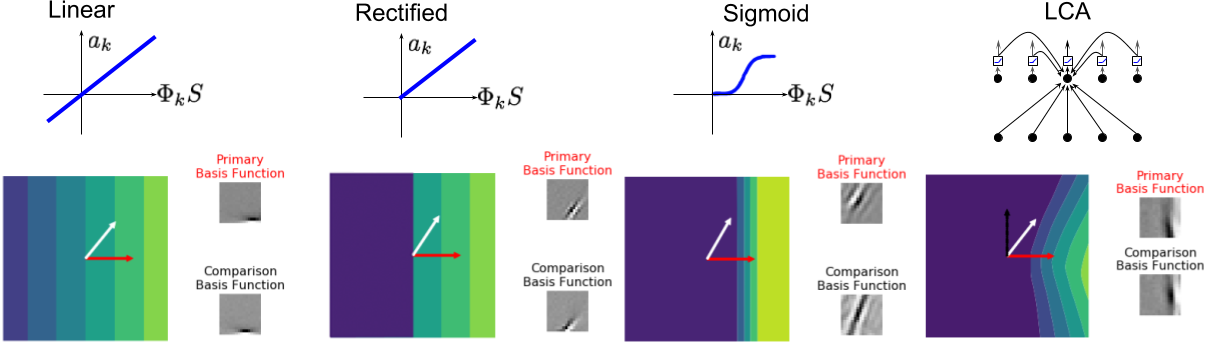
\includegraphics[width=\columnwidth]{Figures/iso_contour_comparison.png}}
\end{center}
%\vskip -0.3in
\caption{Empirically measured iso-response contours. A fine sampling of points in the 2D plane are injected into the high dimensional image space and used as inputs to a target model neuron, $a_{k}$. The color value indicates a binned normalized response magnitude of the neuron. The red arrow is the weight vector for the neuron, $\phi_{k}$. The white arrow is an alternate neuron's weight vector.}
\label{fig:iso_contours}
\end{figure}

%A histogram of 2nd order coefficients for polynomial fits to the lines in the middle plot. Negative coefficients indicate exo-origin curvature, which tells us that this neuron exhibits exo-origin curvature in all orthogonal directions tested.

\subsection{Population nonlinear neurons can be more robust to adversarial examples}
It is important to determine the shape of an individual neuron’s response contours for a large number of planes to better understand its high-dimensional geometry.  To do this, we used two different methods for choosing image planes. For both methods, we defined the horizontal axis as the weight vector (or basis function) for the target neuron. For the first method, we found a set of random vectors that are orthogonal to our target neuron’s weight vector and compute curvature in each plane. For the second method we start by finding another neuron’s weight vector that has a nonzero inner-product with our target neuron’s weight vector (and thus they are not orthogonal). Next, we used the Gram-Schmidt process to find a vector that is orthogonal to our target neuron, but coplanar with our second neuron. This method will increase the likelihood of competition between neurons, and thus increases the curvature. The result is shown in Figure \ref{fig:figure} and indicates that the neuron’s high-dimensional iso-response geometry is cone shaped, with negative curvature in every direction.

\begin{figure}[h]
%\vskip -0.05in
\begin{center}
\centerline{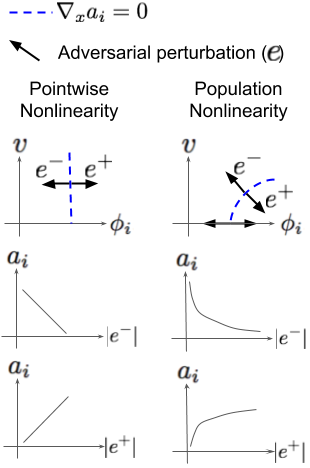
\includegraphics[width=0.5\columnwidth]{Figures/adversarial_gradients_iso_contours.png}}
\end{center}
%\vskip -0.3in
\caption{Adversarial gradients (dark arrows) are always orthogonal to the iso-response contours (blue dashed line).$\Phi_{k}$ indicates a weight vector for the neuron $a_{k}$, and $v$ represents a random orthogonal direction.}
\label{fig:adv_grads}
\end{figure}

Recall that the adversarial objective in equation \ref{eq:adv_metric} has an absolute value and is thus bi-directional. For a locally linear approximation of an untargeted attack, these two directions are equal. However, if we impose a rectifying constraint on our neuron outputs, then the two solutions are not equal for an individual neuron. For a sufficiently large $e$, the direction that lowers $a_{k}$ to below threshold will result in $f(s+e)=0$, i.e. $\max_{e^{-}}|f(s+e)-f(s)| = f(s)$. In other words, for rectified units, $\max_{e^{-}}|f(s+e)-f(s)|$ could be less than $\max_{e^{+}}|f(s+e)-f(s)|$. This would not be known to a simple gradient method for computing an non-targeted adversarial attack, such as that proposed in equation \ref{eq:adv_metric}. However, in practice actual adversarial attacks have an additional goal in mind: to produce an output that is reasonable for some \emph{other} data sample. Turning off all of the units in a layer is not a solution to this problem, so some set of adversarial perturbations must be in the $e^{+}$ direction. By definition, these perturbations will have greater contribution to the model's output than $e^{-}$ perturbations.

The Locally Competitive Algorithm (LCA) is a neural network with population nonlinearities that exhibits exo-origin bent iso-response contours. If the LCA is also rectified, then the $e^{-}$ direction will eventually turn off units. From Figure \ref{fig:adv_grads} one can deduce that the only $e^{+}$ direction that will cause $a_{k}$ to grow without bound is along $\Phi_{k}$. What's more, \emph{all} directions that increase $a_{k}$ are towards, or along, $\Phi_{k}$. From this analysis we present three hypotheses:

\begin{itemize}
  \item Adversarial attacks on networks with exo-origin bent contours will be more aligned with the their weight vectors than attacks on networks with straight contours. If the weight vectors are data aligned then this will result in adversarial attacks that are data aligned.
  \item Rectified LCA should be resistant to unbounded adversarial attacks.
  \item Non-rectified LCA should be more susceptible to adversarial attacks than rectified LCA.
  \item More overcompleteness causes more bending of the iso-response contours \parencite{golden2016conjectures}, which will result in better adversarial defense.
\end{itemize}

In the following section we will outline several models used for our experiments as well as the experiments performed. Then we will present results that support the above hypotheses. Finally we will discuss the implications of these results and propose continued directions for research.

\section{Experimental models}\label{sec:models}
\subsection{The Locally Competitive Algorithm} \label{sec:lca}
The Locally Competitive Algorithm finds a solution to the following optimization problem:

\begin{equation}\label{eq:energyfunc}
    \argmin\limits_{a}
        \left( E =
            \overbrace{ \tfrac{1}{2} \| s - a \Phi^{\top} \|_{2}^{2} }^\text{Preserve Information} +
        \overbrace{ \lambda \sum\limits_{i=1}^{M}C(a_{i}) }^\text{Limit Activations} \right),
\end{equation}

where $s$ is an input vector, $a$ is a neural activity vector, $\Phi$ is a weight matrix, and $C(\cdot)$ is a cost function on the activations, which will be the $l_{1}$ norm of the activity vector for our preliminary study: $C(a_{k}) = |a_{k}|$. The cost function has a considerable impact on the network dynamics \parencite{rozell2008sparse} and alternatives are of interest for future work. The LCA describes an activation coefficient, $a_{k}$, as the thresholded output of a model neuron's internal state, $u_{k}$. The network finds a minima to equation \ref{eq:energyfunc} by following its gradient:

\begin{displaymath}
    \dot{u_{k}}(t) &\propto - \frac{\partial E(t)} {\partial a_{k}(t)}
\end{displaymath}

\begin{equation}\label{udot}
    \dot{u_{k}}(t) &= \frac{1}{\tau} \left[\Phi^{\top}_{k}s - \sum_{m \neq k}^{M}G_{k,m}a_{m}(t) - f_{\lambda}(a_{k}(t)) \right],
\end{equation}

where $\tau$ is a time constant, $G = \Phi^T\Phi$, and $f_{\lambda}(a_{k}(t)) = a_{k}(t) + \lambda \frac{\partial C(a_{k}(t))}{\partial a_{k}(t)}$. A neuron's output is computed using a thresholding function $a_{k}(t) = T_{\lambda}(u_{k}(t)) = \text{ReLU}(f_{\lambda}^{-1}(u_{k}(t)))$:

\begin{equation}\label{lcathresholdfunc}
    T_{\lambda}(u_{k}(t)) = \left\{
    \begin{aligned}
        u_{k}(t)-\lambda,\;\; &u_{k}(t)\; >\; \lambda \\
        0,\;\; &u_{k}(t)\; <\; \lambda
    \end{aligned}
    \right.
\end{equation}

Our model differs from the original citation in that we rectify our output thresholding function. Finally, we can update our weights using stochastic gradient descent for a given sparse code of a batch of inputs:

\begin{equation}\label{phiupdate}
  \Delta \Phi = \eta (s - a(t=T)\Phi^{\top})^{\top} a(t=T),
\end{equation}

where $T$ is the total number of inference steps.

We suggest that the LCA requires stronger adversarial perturbation magnitudes to achieve the same change in the network output when compared to more standard feedforward autoencoders. Additionally, adversarial perturbations for the LCA are more aligned with the data than those for the alternative models tested. We have shown that both of these properties can be explained by an LCA neuron's exo-origin bent iso-response contours. We believe that this study synergizes with the works of \parencite{zhu2013visual} and \parencite{golden2016conjectures}, which together suggest that explaining-away process inherent in the sparse coding model produces a more selective and robust code of input data.

%\subsection{Comparison Models}
%We compared the LCA responses against a variational autoencoder \parencite{kingma2013auto}.
%The comparison models are:
%  * MLP (tensorflow tutorial)
%  * Sparse Autoencoder
%  * [Deep/Shallow] Variational Autoencoder
%  * LISTA

\section{Experiments on the MNIST dataset}
From the above analysis, we hypothesized that adversarial attacks for the LCA would be more data aligned than those for an autoencoder using pointwise nonlinearities. To begin testing this hypothesis, we followed the procedure outlined in \parencite{kos2018adversarial} to construct generative adversarial attacks. We consider the LCA as an autoencoder model, $\hat{s}=f(s)$, which encodes images into a latent space and then produces reconstructions from this encoding. We compare the LCA against the following models:

\begin{itemize}
  \item A sparse autoencoder (SAE, \parencite{ng2011sparse}) with a single overcomplete hidden layer that uses a pointwise sigmoid nonlinearity.
  \item A pointwise rectified (ReLU) autoencoder \parencite{citation} with a single overcomplete hidden layer.
  \item A deep bottleneck pointwise rectified (ReLU) autoencoder.
  \item A deep variational autoencoder \parencite{kingma2013auto}.
\end{itemize}

  For the attack, an input image, $s$, was minimally perturbed before being passed through the autoencoder to produce a reconstruction of an entirely different target image, $s_{t}$. First, we found that the angle of the perturbed inputs, $s^{*}$, were closer to the target for LCA than for the SAE (Figure \ref{fig:cosine_similarity}). We found that this performance difference was consistent through a sweep of attack parameters \ref{fig:kos_attack}. Next, we found that for attacks that did not include a clipping step to force the perturbation to be a certain size, the SAE perturbation grew without bound while the LCA perturbation settled to a fixed distance from the input (Figure \ref{fig:figure}). Finally, to test whether this phenomena could result in improved adversarial robustness for classification networks, we compared a 2 layer neural network (MLP) with ReLU nonlinearities trained to identify the digit classes in the MNIST dataset against a single layer ReLU classifier (SLP) trained on the latent code produced by LCA. We found that the LCA+SLP model required a larger perturbation from the original input (as measured by mean squared error, MSE) for equal adversarial confidence than the MLP. Additionally, we found that the perturbations themselves were more semantically meaningful for the LCA+SLP than for the MLP (Figure \ref{fig:latent_attac_mse}).

%In the following we will conduct several different adversarial attack experiments on a variety of models. The attacks are:
%  * Generative adversarial attack (kos)
%      - explanation
%  * Pixel classification attack
%      - explanation
%  * Latent classification attack
%      - explanation

\subsection{LCA Adversarial Attacks are Data Aligned}
In section \ref{neuron}, we showed that adversarial gradient directions for LCA neurons will point in data directions. To assess whether this result extends to the entire network, we measured the cosine similarity between an input image and a successful adversarial perturbation. Figure \ref{fig:cosine_similarity} demonstrates that adversarial perturbations for the LCA have a higher cosine similarity to the target image in a generative adversarial attack \parencite{kos2018adversarial} than the SAE. This indicates that the perturbations are more closely aligned to data directions, which should result in more semantically meaningful perturbations.

\begin{figure}[h]\label{fig:cosine_similarity}
%\vskip -0.05in
\begin{center}
\centerline{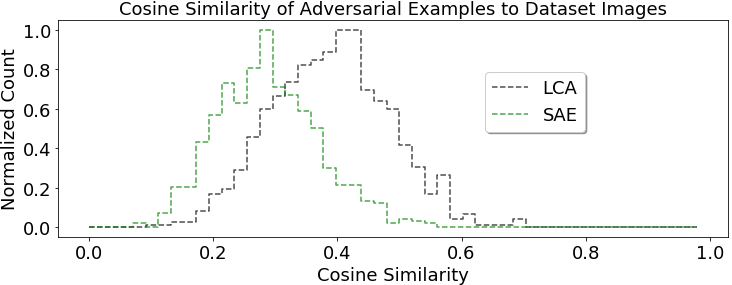
\includegraphics[width=\columnwidth]{Figures/cosyne_similarity.png}}
\end{center}
%\vskip -0.3in
\caption{Adversarial attacks using gradients from the LCA have a larger cosine similarity to dataset images than attacks for the SAE. Following \parencite{kos2018adversarial}, we attacked each model using a target image that was an alternate image from the dataset. The histograms are computed over 800 image examples.}
\end{figure}

To understand how adversarial attacks transfer between these models, we produced adversarial images for each one and test how adversaries generated for one model affect another. The data-aligned perturbations can explain why adversarial images for LCA transfer to SAE and VAE but not the other way around \ref{fig:figure}.

\subsection{Pixel classification attack}
The standard attack method for classification networks is to perturb input pixels to result in misclassification. One proposed defense against this type of attack is to preprocess the image pixels with a denoising autoencoder that would produce reconstructions void of the adversarial pixel perturbations. However, it has been shown that if one backpropagates the adversarial loss through the autoencoder network, then it is still possible to adversarially attack the network. Here we show that the LCA model outperforms the VAE and SAE networks as a preprocessing \"firewall\" against the adversarial attacks.

\subsection{Generative adversarial attacks}
Recent results from \citet{kos2018adversarial} show that adversarial stimulus can be constructed for generative models. This is especially compelling because generative models are explicitly trained to preserve information about the input and produce a veridical reconstruction, whereas classification networks are typically trained to throw away large amounts of information and only preserve that which is relevant for the given task. We show that the LCA model is robust against generative adversarial attacks when compared to the SAE and VAE networks.

%
% * best solution is identity, but that is not an interesting solution
% * this attack prefers simpler models
% * which is why we include sae w/ tied weights
%

\begin{figure}[h]\label{fig:kos_attack}
%\vskip -0.05in
\begin{center}
\centerline{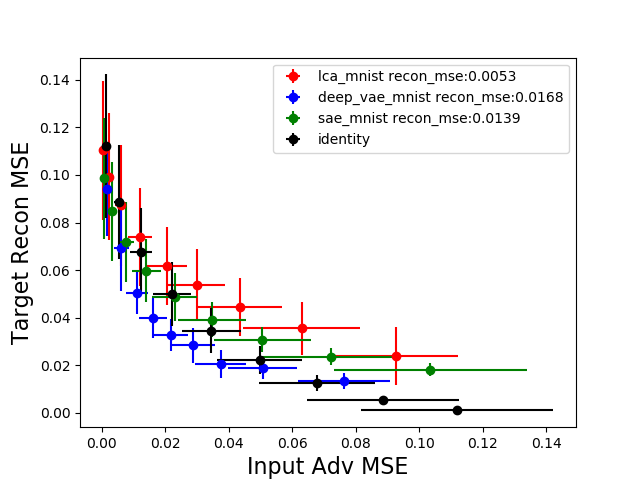
\includegraphics[width=\columnwidth]{Figures/recon_mult_tradeoff.png}}
\end{center}
%\vskip -0.3in
\caption{TODO}
\end{figure}

\subsection{Latent classification attack}
The lateral connectivity in the LCA network is utilized via a recurrent computation. These dynamics facilitate a form of explaining away, where neurons that have a high degree of correspondence with the input stimulus suppress other neurons in the network. This results in the network ignoring input pixels that are not aligned with primary data directions. To better understand the role of the recurrent computation, we trained a network that acts as an unrolled version of LCA, where the lateral connectivity and feedforward weight matrices are learned. The LISTA model was demonstrated by Gregor et al. \citeyearpar{gregor2010learning} to show that a network with many fewer inference steps can produce codes that have a small Euclidean distance to the outputs of sparse coding. We trained three LISTA models with 5, 20, and 50 layers. All three models were trained to produce codes that had approximately the same $L_{2}$ distance from the codes produced by LCA. We show that the LISTA network does not perform as well as LCA at defending against adversarial attacks and that the deeper LISTA networks perform better.

\begin{figure}[h]
\vskip -0.05in
  \begin{subfigure}
    \centering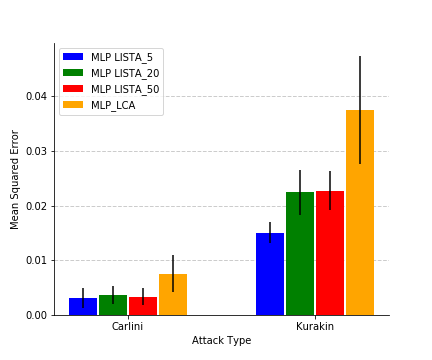
\includegraphics[width=\columnwidth]{Figures/latent_clf_attack_mse.png}
  \end{subfigure}
  \begin{subfigure}
    \centering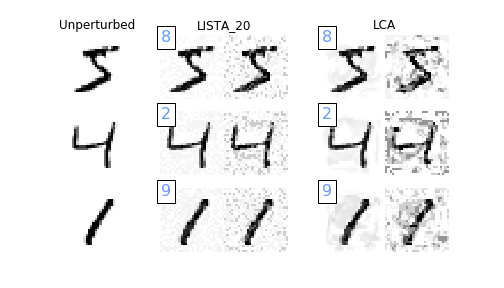
\includegraphics[width=\columnwidth]{Figures/latent_clf_attack_ex.png}
  \end{subfigure}
\caption{LCA better protects against latent classification attacks. We generated adversarial examples from equal-sized MLPs trained from the latent codes of each model. MSEs were calculated between the original image and the perturbed image.   Error bars indicate standard deviation for 100 example inputs.}
\label{fig:latent_attac_mse}
\end{figure}

\subsection{Attacks with the CIFAR dataset}
The LCA objective is derived from a model of natural images, so we believe the network will exhibit stronger aversion to adversarial perturbations.
%%%% From paper

\section{Explaining increased orientation selectivity}
A longstanding hypothesis in visual neuroscience is that sensory neurons are adapted to natural image statistics to produce an efficient code. Independent Component Analysis (ICA) has been proposed as a normative model for simple cells in V1 based on its ability to reduce higher-order redundancy in natural images. When applied to natural images, the filters that emerge resemble the localized, oriented, and band-pass receptive fields of V1 neurons. However, quantitative analyses of the coding efficiency of ICA show that the neural code it produces fails to provide any appreciable gain in redundancy reduction beyond second-order methods such as PCA. This result appears to challenge the higher-order redundancy reduction account of V1 function. We explain these findings by distinguishing oriented filters from orientation \textit{selectivity} and show that ICA's linear encoding scheme fails to implement genuine orientation selectivity, which limits its capacity to learn an efficient code. We show that sparse coding, a related model with a nonlinear encoding scheme that produces orientation selective neurons, is able to achieve a more efficient code than both ICA and PCA when evaluated in the rate-distortion framework, thus providing renewed support for the efficient coding account of V1 receptive field properties.

A long-standing hypothesis in sensory neuroscience proposes that a primary function of early sensory processing is to form an efficient, redundancy-reduced code of the input that maximizes the brain's limited computational and biological resources while making explicit the statistical structure of the input \parencite{barlow2001redundancy}. This hypothesis predicts that the response properties of sensory neurons should be adapted to the statistical structure of their input.

In support of this hypothesis, a number of the response properties of visual neurons have been reproduced by optimizing redundancy-reducing linear transformations on natural images \parencite{atick1990towards}. For example, a symmetric decorrelation transformation of natural images yields center-surround receptive fields \parencite{atick1990towards}, and Principal Component Analysis (PCA) applied to color images yields the luminance, red-green, and blue-yellow channel observed in the opponent color coding of retinal ganglion cells \parencite{ruderman1998statistics, buchsbaum1983trichromacy}. When higher-order correlations are additionally reduced, localized and oriented band-pass filters that resemble the orientation-selective receptive fields in V1 emerge \parencite{bell1997independent, olshausen1999probabilistic}. It has thus been proposed that the oriented filters in V1 function to remove higher-order correlations.

Orientation selectivity is a striking feature of the response properties of simple cells in V1. Since the discovery of orientation selectivity in Hubel and Wiesel's Nobel Prize-winning work, the mechanism for the computation has remained unclear. A common point of confusion in the field has been the assumption that a neuron with an locally oriented receptive field will exhibit orientation selectivity. Here, we will argue that orientation selectivity requires a non-linear encoding process in addition to an oriented receptive field.

Independent Component Analysis (ICA) is one of the most widely used image coding algorithms and has been proposed as a model for simple cells in V1 \parencite{bell1997independent}. The ICA algorithm explicitly optimizes for higher-order redundancy reduction, aiming to to reconstruct the input image as a linear superposition of a set of basis functions while minimizing the mutual information between those bases.

\citeit{eichhorn2009natural} compare the  coding efficiency of ICA and PCA to obtain the surprising result that ICA performs no better than PCA on a rate-distortion trade-off metric. ICA is trained with the objective of minimizing the joint entropy of the activations and learns oriented filters that suggest it has succeeded in modeling higher-order pixel correlations, while PCA is a second-order method that does not learn oriented filters. \citeit{eichhorn2009natural} argue that if ICA had succeeded at capturing higher-order statistics, it should show an advantage in the rate-distortion trade-off.

We present an alternate explanation of these findings by distinguishing \textit{orientation selectivity} from \textit{oriented filters}. Neurons achieve orientation selectivity via a fundamentally nonlinear process, as exhibited by nonclassical receptive field (nCRF) effects such as cross-orientation suppression \parencite{golden2016conjectures, zhu2013visual}. We argue that although the ICA optimization algorithm is able to learn oriented filters, ICA's linear encoding process limits its capacity to perform genuine orientation selectivity, which in turn limits its capacity to produce an efficient code. \citeit{zhu2013visual} demonstrate that sparse coding is able to provide a parsimonious explanation of both classical and nonclassical receptive field properties using a neural network implementing sparse coding \parencite{zhu2013visual}. Here, we replicate the rate-distortion analyses from \citeit{eichhorn2009natural} using the sparse coding network described by \citeit{zhu2013visual} to show that a nonlinear encoding process produces more efficient codes to linear encoders. To assess the degree of orientation selectivity for ICA neurons, we replicate the cross-orientation suppression experiment performed by \citeit{zhu2013visual} with both sparse coding and ICA networks.


\subsection{Rate-distortion analyses}
The Shannon standard for evaluating the efficiency of lossy continuous codes is the rate-distortion framework \parencite{cover2012elements}. \citeit{eichhorn2009natural} compare the  coding efficiency of ICA and PCA and find that PCA performs \textit{better} than ICA in terms of the rate-distortion trade-off. This result is surprising in that ICA is explicitly trained with the goal of minimizing the joint entropy of the activations and learns oriented filters that would suggest that it achieved the goal of modeling higher-order correlations, while PCA is a second-order method that does not learn oriented filters.

We resolve this apparent paradox by distinguishing \textit{orientation selectivity} and \textit{oriented filters}. Neurons achieve orientation selectivity via a fundamentally non-linear process, as exhibited by non-classical receptive field (nCRF) effects such as contrast invariant tuning and cross-orientation suppression \parencite{ferster2000natural,  zhu2013visual}. We argue that although the ICA optimization algorithm is able to learn oriented filters, ICA's linear encoding process limits its capacity to perform genuine orientation selectivity, which in turn limits its capacity to produce an efficient code. Sparse coding is unique in its ability to provide a parsimonious explanation of both classical and non-classical receptive field properties \parencite{zhu2013visual, golden2016conjectures}. Although nCRF effects are typically modeled individually, \citeit{zhu2013visual} show that a wide variety of these effects are emergent properties of a neural network implementing sparse coding. * something about LCA * These findings suggests the primacy of efficient coding in V1. This explanation only holds, however, if sparse coding can be quantitatively shown to achieve a gain in coding efficiency beyond second-order methods. Here, we replicate the rate-distortion analyses from \citeit{eichhorn2009natural} and show that sparse coding's non-linear encoding process enables codes that are lower entropy than those learned by ICA or PCA while being more perceptually robust to increasingly coarse quantization.


\subsection{Methods and Results}
We train sparse coding \parencite{rozell2008sparse}, ICA \parencite{bell1997independent}, and PCA on 1 million 16 x 16 pixel grayscale image patches extracted from images in the van Hateren dataset of natural scenes, which have been transformed to log intensity and standardized to zero mean and unit variance \parencite{vanHateren1998independent}. Using the learned filter matrices, we compute model activations for a test set of 100,000 patches and uniformly quantize these activations with varying degrees of granularity. For each level of granularity, we compute a reconstruction of the test input using the quantized activations and compute the mean squared error. Figure \ref{fig:rd_curve} plots the rate (mean marginal discrete entropy of the activations) against the distortion (mean squared error).

%\begin{figure}[ht]
%\vskip 0.1in
% \centering \includegraphics[width=\linewidth]{figures/rd_curves.png}
% \caption{Discrete entropy vs. reconstruction error for sparse coding, PCA, and ICA.}
%\vskip -0.2in
%\label{fig:rd_curve}
%\end{figure}

Results for sparse coding models trained with different values of $\lambda$ are shown, where a larger $\lambda$ indicates higher sparsity. We replicate the findings from \citeit{eichhorn2009natural} that (orthogonal) PCA  performs slightly better than ICA in the rate-distortion trade-off. Sparse coding shows an advantage over both ICA and PCA. Additionally, we find that representations that are more sparse are capable of achieving increasingly lower rates.
Figure \ref{fig:recons} shows an example reconstruction in the highly lossy (low entropy) regime. For a mean marginal entropy of $H\approx 0.4$, sparse coding shows an advantage in perceptual quality, as well as a quantitative advantage in terms of mean squared error.

%\begin{figure}[ht]
%\vskip 0.1in
% \centering
% \includegraphics[width=\linewidth]{figures/baboon_4_square.png}
% \caption{Lossy reconstructions for quantized activations with mean marginal entropy $H\approx 0.4$}
%\vskip -0.2in
%\label{fig:recons}
%\end{figure}


\subsection{Discussion}
Our results suggest the importance of nonlinear encoding for learning efficient codes of natural images and demonstrate that orientation \textit{selective} neurons are capable of reducing higher-order redundancy. We show that although the ICA algorithm is able to learn oriented filters, ICA's linear encoding process limits its capacity to perform genuine orientation selectivity, which in turn limits its capacity to produce an efficient code. 

Although sparse coding produces a more efficient representation of natural image and neurons that have a higher degree of orientation selectivity than ICA, the model is nonetheless fundamentally limited in its capacity to fully characterize the statistics of natural scenes because it assumes a linear generative model and the light that forms images is combined in a non-linear fashion, such as by occlusion. In future work we plan to extend our analysis to hierarchical models of natural scenes that may achieve greater gains in coding efficiency.

The efficient coding hypothesis was initially posed in terms of redundancy reduction \parencite{barlow1961possible}, under the hypothesis that the brain may seek an efficient code of the input in order to minimize the number of neurons required to represent the signal. Anatomical evidence tells us, however, that the V1 expands the image representation coming from LGN by having many more outputs than inputs \parencite{olshausen2003principles} Thus, redundancies are actually \textit{created} in the perceptual process. The goal of cortical processing, then, cannot be said to be redundancy reduction and simple compression.

As an alternative, several researchers have argued that the goal of perception cannot be discussed in isolation from action; an organism forms perceptual representations for the purpose of directing its behavior towards the achievement of desirable outcomes and away from undesirable ones \parencite{barlow2001redundancy, simoncelli2001natural}. From this perspective, the brain aims to extract the statistical structure of the input in order to form a``meaningful'' representation that recovers the environmental causes of the sensory data, which it can use to guide action. Along these lines, the efficient coding hypothesis has been revised to emphasize redundancy \textit{representation} rather than reduction \parencite{barlow2001redundancy}. Redundancies in the input signal indicate structure in the environment. An encoding that makes these redundancies explicit encodes the causal and statistical structure of the environment, which the organism can exploit to plan and direct behavior.

Sparse coding performs redundancy representation rather than redundancy reduction. A sparse code is a highly redundant code It has been demonstrated that a typical redundancy reducing code--which would form a distributed representation of the input with a high activity ratio--would actually lead to large errors in estimates of the frequency of a particular input, since many neurons are active in response to both the input of interest as well as other stimuli \parencite{gardnermedwin2001limits}. A sparse code, in which the elements of the learned dictionary occur independently in the environment, is a factorial code; the probability of any composite image is simply the product of the probabilities of the components. Any deviations from this rule signal a previously unknown statistical dependency to be learned.

 An efficient code exploits the redundancies in the input signal. The objective of early sensory processing was initially described as redundancy reduction. The redundancy reduction hypothesis was partially motivated by the observation that a significant information bottleneck exists in the first stage of visual processing; most mammals have vastly more photoreceptors than fibers in the optic nerve, which suggests that significant compression must occur in the first stage of processing. However, at moderate to high luminance levels, only a small subset of the photoreceptors are operating within their dynamic ranges; thus the reduction in capacity may be smaller than initially implied. Further, beyond the optic nerve, the number of neurons involved in subsequent layers of processing generally increases, which means that redundancies are actually created in the perceptual process. The goal of early vision, then, cannot be said to be redundancy reduction. From a functional standpoint, several researchers have also argued that the goal of perception is not simple compression; an organism forms perceptual representations in order to direct its behavior towards the achievement of desirable outcomes and away from undesirable ones \parencite{barlow2001redundancy, simoncelli2001natural}. From this standpoint, one can argue that brain aims to extract the statistical structure of the input in order to form a \textit{meaningful} representation that recovers the environmental causes of the sensory data, which it can use to guide action.
 
 Along these lines, the efficient coding hypothesis has been revised more recently to emphasize redundancy representation rather than reduction \parencite{barlow2001redundancy}. Redundancies in the input signal indicate structure in the environment. An encoding that makes these redundancies explicit encodes the causal and statistical structure of the environment, which the organism can exploit to plan and direct behavior. Barlow further argues that to facilitate the identification of the statistics of the environment, neural responses should form a sparse code of the input. He notes that a typical redundancy-reducing code would be a distributed representation of the input with a high activity ratio–that is, a large percentage of active neurons, each of which is frequently active across different inputs. Such a code will lead to large errors in estimates of the frequency of a particular input, since many neurons are active in response to both the input of interest as well as other stimuli. A sparse code, in which the elements of the learned dictionary occur independently in the environment, would form a factorial code, in which the probability of any composite image is simply the product of the probabilities of the components. Any deviations from this rule would signal a previously unknown statistical dependency to be learned.
 
%%%% From paper
Although the softmax nonlinearity used in most classification models is a population nonlinearity, we hypothesize that an adversarial image perturbation can produce adversarial inputs to the softmax, negating it's ability to protect the network against the attack.

Additional control models need to be explored, including alternative population nonlinearities such as those present in Boltzmann machines \parencite{salakhutdinov2009deep}, divisive normalization \parencite{balle2016end}, and local response normalization \parencite{krizhevsky2012imagenet}. Each of these nonlinearities has had significance in the deep learning and neuroscience communities. The iso-response analysis provides a methodology for contrasting them and will give us valuable insight into how each of them may respond to adversarial attacks. We also wish to scale up the models to include larger datasets of more naturalistic images. 

Hierarchical extensions to the sparse coding model \parencite{chen2018sparse} have been shown by our group to perform a better job of mapping input data onto a smooth manifold. We hypothesize that this will further increase the semantic relevance and model robustness for adversarial perturbations. We intend to include the model defined in \parencite{chen2018sparse} in our future analysis to explore how the adversarial and iso-response properties change as we increase the network depth.

This methodology has a high potential for impact in the deep learning community. We advocate for biologically motivated computations that go beyond the simple pointwise nonlinear model. We have shown that these types of networks learn a more robust representation of data without tedious and biased human labeling. We also provide strong theoretical support for our hypotheses and an analysis method that allows us to fully characterize how the more complicated neurons will respond to input perturbations.
%%%%

\section{Explaining extra-classical receptive field effects}
Golden, explaining others.


\section{Applications to physiological neuroscience}
Use this method to probe neuron contours.\label{ch:hierarchical_sc}
\chapter{Conclusions}

\section{stuff}
Bringing it all together...

\appendix
\chapter{appendix}

\clearpage
\printbibliography

\end{document}